\chapter{Detector magnet system}
\label{Chapter:Magnet}


\section{General Design Considerations}
The CEPC detector magnet system is designed to provide an axial magnetic field over the tracking volume, a diameter 6.8 m over a length of 8.05 m, particle detectors within this volume will measure the trajectories of charged tracks emerging from the collisions. Based on the study of the compensating magnet of CEPC, a 3 T central field of detector superconducting solenoid is more reality to construct the CEPC compensation solenoid which making full cancelation to avoid disturbance to the beam with technologies to be developed in coming years, comparing the 3.5 T solenoidal field proposed in pre-CDR.


This chapter contains all the activities related to the design of field distribution, solenoid coil, specific superconductor, cryogenics, quench protection and power supply, and the yoke.
In this report, for the first time, we explored the possibility of using HTS to build CEPC detector magnet. Benefit from the development of high Tc superconductor in recent years, the advantages by using YBCO winding is higher operating temperature, better stability to resist transient disturbances when operating the magnet.


We also discussed on the choice between iron yoke design and dual solenoid scenario. The baseline design iron yoke consists of barrel yoke and end yoke. It has three main functions: first is shielding the magnetic field; second is providing the install space for the muon detector which sandwiched between the iron plates; in addition, the yoke serves as the main mechanical structure of the CEPC detector. However, the second one which called active shielding design has been widely used in for commercial MRI magnets, this scenario will not use iron yoke, and it has large impact on muon detector design.
%
\section{The Magnetic Field Requirements and Design}
\subsection{Main parameters}


The CEPC solenoid main parameters are given in Table 6.1. The 7.6 m long CEPC detector coil is composed of 5 modules. This batches the construction easiness and risks including superconducting wire selection, fabrication of the external support, winding and impregnation, transport and handling. The design enables the possibility to use shorter unit lengths of superconducting conductor (1.65 km) and join them in known positions and in low field regions, on the outer radius of the solenoid. The difference compared to PreCDR is that the central magnetic field changes from 3.5 T to 3 T. The geometry size is the same with 3.5 T design, as shown in Fig. 8.1.
\begin{table}[!h]
	\centering
	\begin{tabular}{c|c|c|c}
		\hline
		The solenoid central field (T) & 3 & Working current (kA) & 15779 \\
		\hline
		Maximum field on conductor (T) & 3.485 & Total ampere-turns of the solenoid (MAt) & 20.323 \\
		\hline
		Coil inner radius (mm) & 3600 & Inductance (H) & 10.46 \\
		\hline
		Coil outer radius (mm) & 3900 & Stored energy (GJ) & 1.3 \\
		\hline
		Coil length (mm) & 7600 & Cable length (km) & 30.35 \\
		\hline
	\end{tabular}
	\caption{main parameters of the solenoid coil}
	\label{tab:structure}
\end{table}
%
\begin{figure}[h!]
\centering
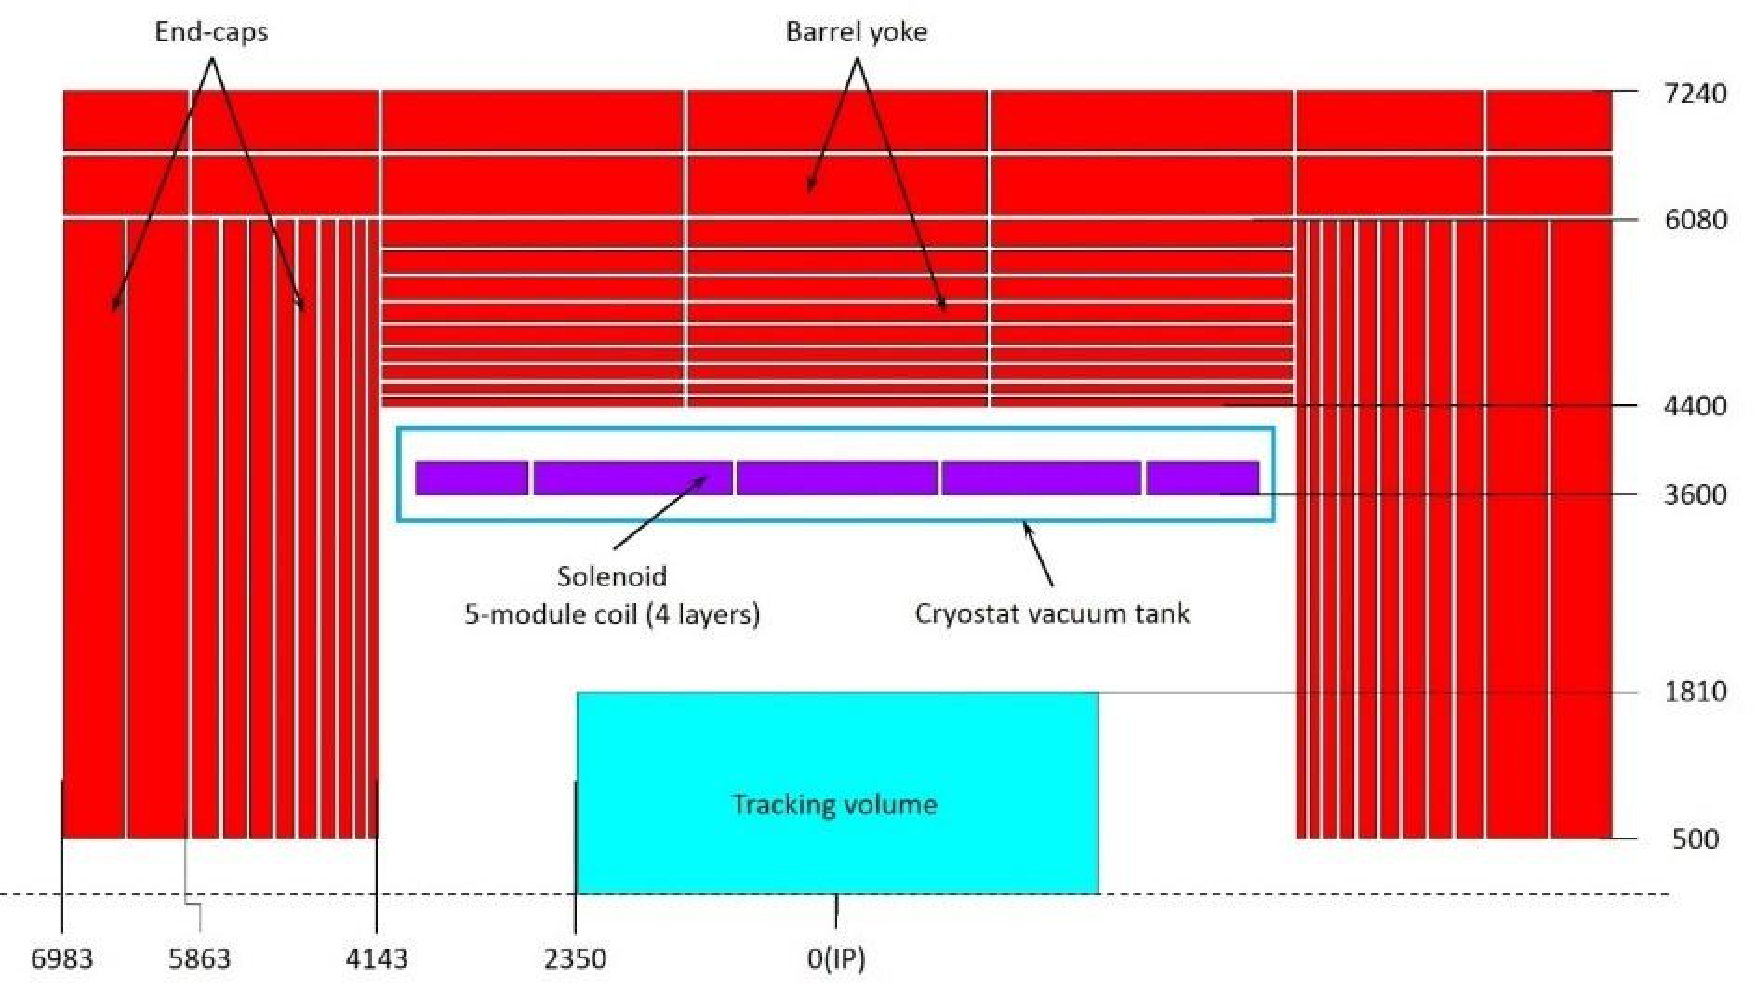
\includegraphics[scale=0.36]{Figures/Magnet/21}
\caption{2D layout of CEPC magnet (mm)}
\label{fig:21}
\end{figure}
%
  There are five modules of the coil. Each module contains 4 layers. The end two modules contain 44 turns per layer. Table 6.2 shows the coil parameters.
  \begin{table}[!h]
	\centering
	\begin{tabular}{c|c|c}
		\hline
		Coil number & layers & Turns per layer \\
		\hline
		1 & 4 & 44 \\
		\hline
		2 & 4 & 78 \\
		\hline
		3 & 4 & 78 \\
		\hline
		4 & 4 & 78 \\
		\hline
        5 & 4 & 44 \\
		\hline
	\end{tabular}
	\caption{ coil parameters}
	\label{tab:structure}
\end{table}
\subsection{Magnetic field design}


In the calculation we use the cable as Fig. 6.2. In the center is the NbTi Rutherford cable, and then is the pure aluminum stabilizer and aluminum alloy reinforcement. The figure shows the parameters of the cable. This model has been used for magnetic field calculation, stress analysis of the coil and quench analysis of the magnet.


Fig. 6.3 shows the magnetic field map of the magnet. The central field is 3 T, the maximum magnet field is 3.5 T. Figure 6.4 gives the main component BZ of the field along the beam axis. Figure 6.5 show the Magnetic flux line distribution of the magnet.
The non-uniformity of Tracking Volume (diameter 3.62m, length 4.7m) is 9.11$\%$. Figure 6.6 show the magnetic field distribution of the Tracking Volume.
$$B_p=\left.\frac{Bmax-Bmin}{Bcenter}\right.=9.11\%$$
%
\begin{figure}[h!]
\centering
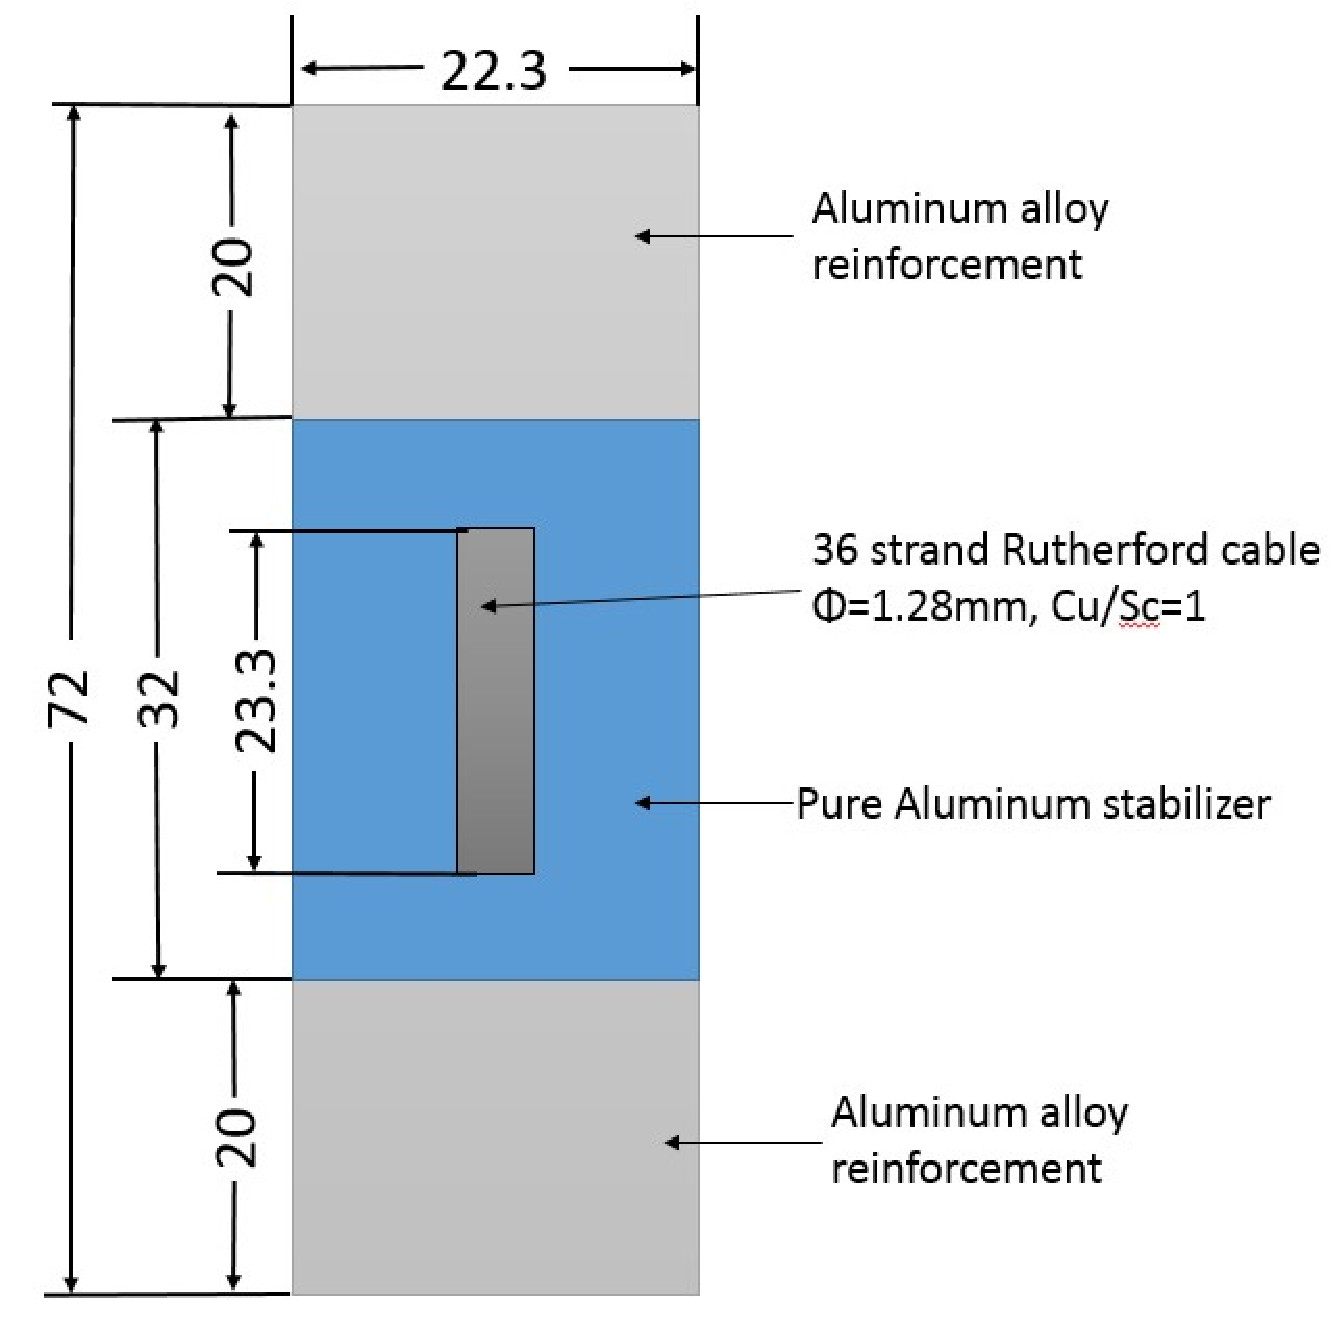
\includegraphics[scale=0.36]{Figures/Magnet/22}
\caption{sketch figure of cable cross section}
\label{fig:22}
\end{figure}
%
\begin{figure}[h!]
\centering
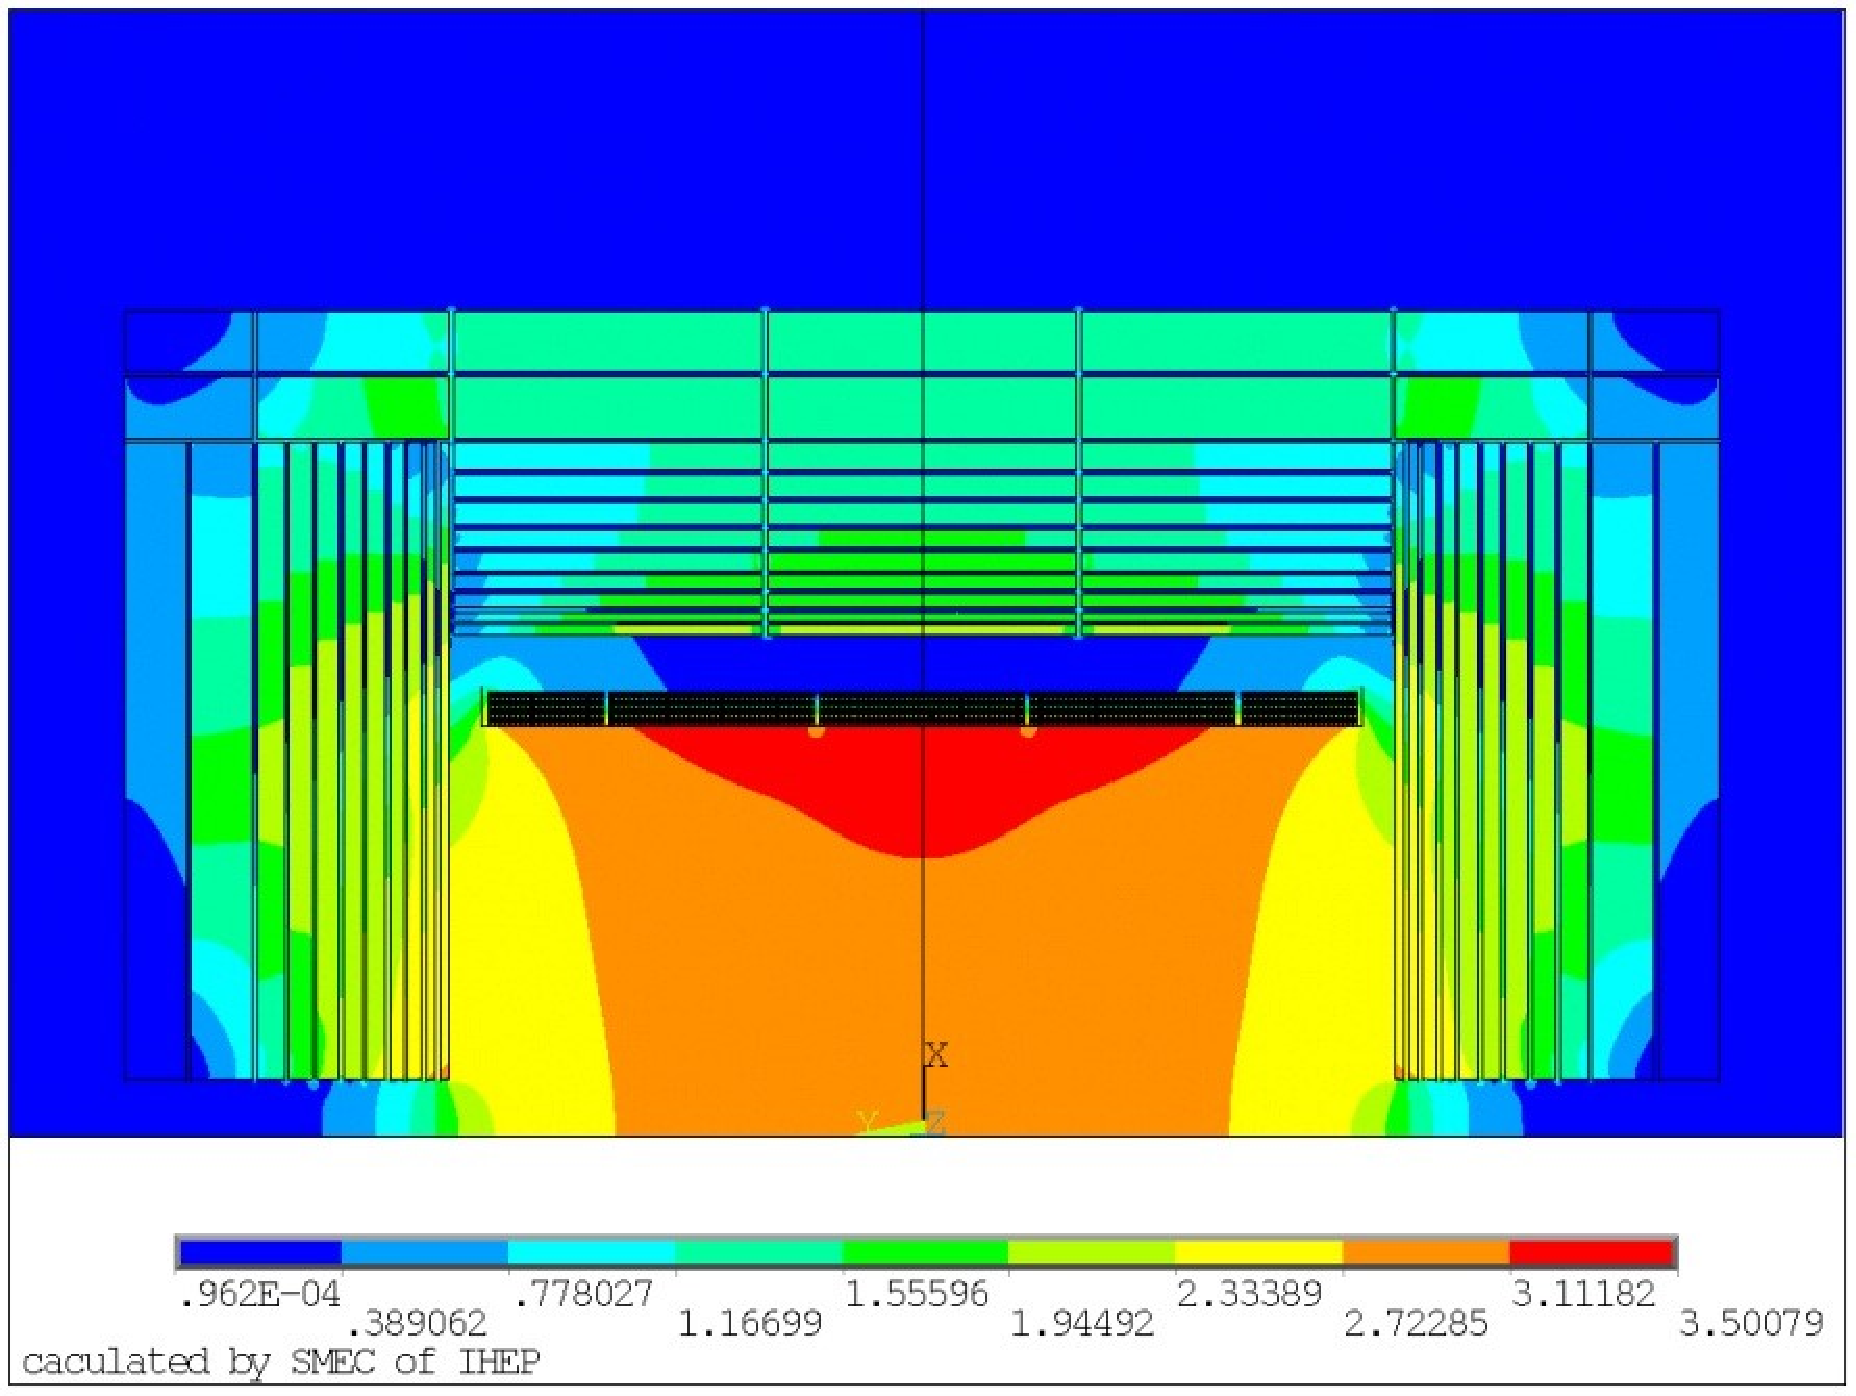
\includegraphics[scale=0.36]{Figures/Magnet/23}
\caption{ Field map of the magnet (T)}
\label{fig:23}
\end{figure}
%
\begin{figure}[h!]
\centering
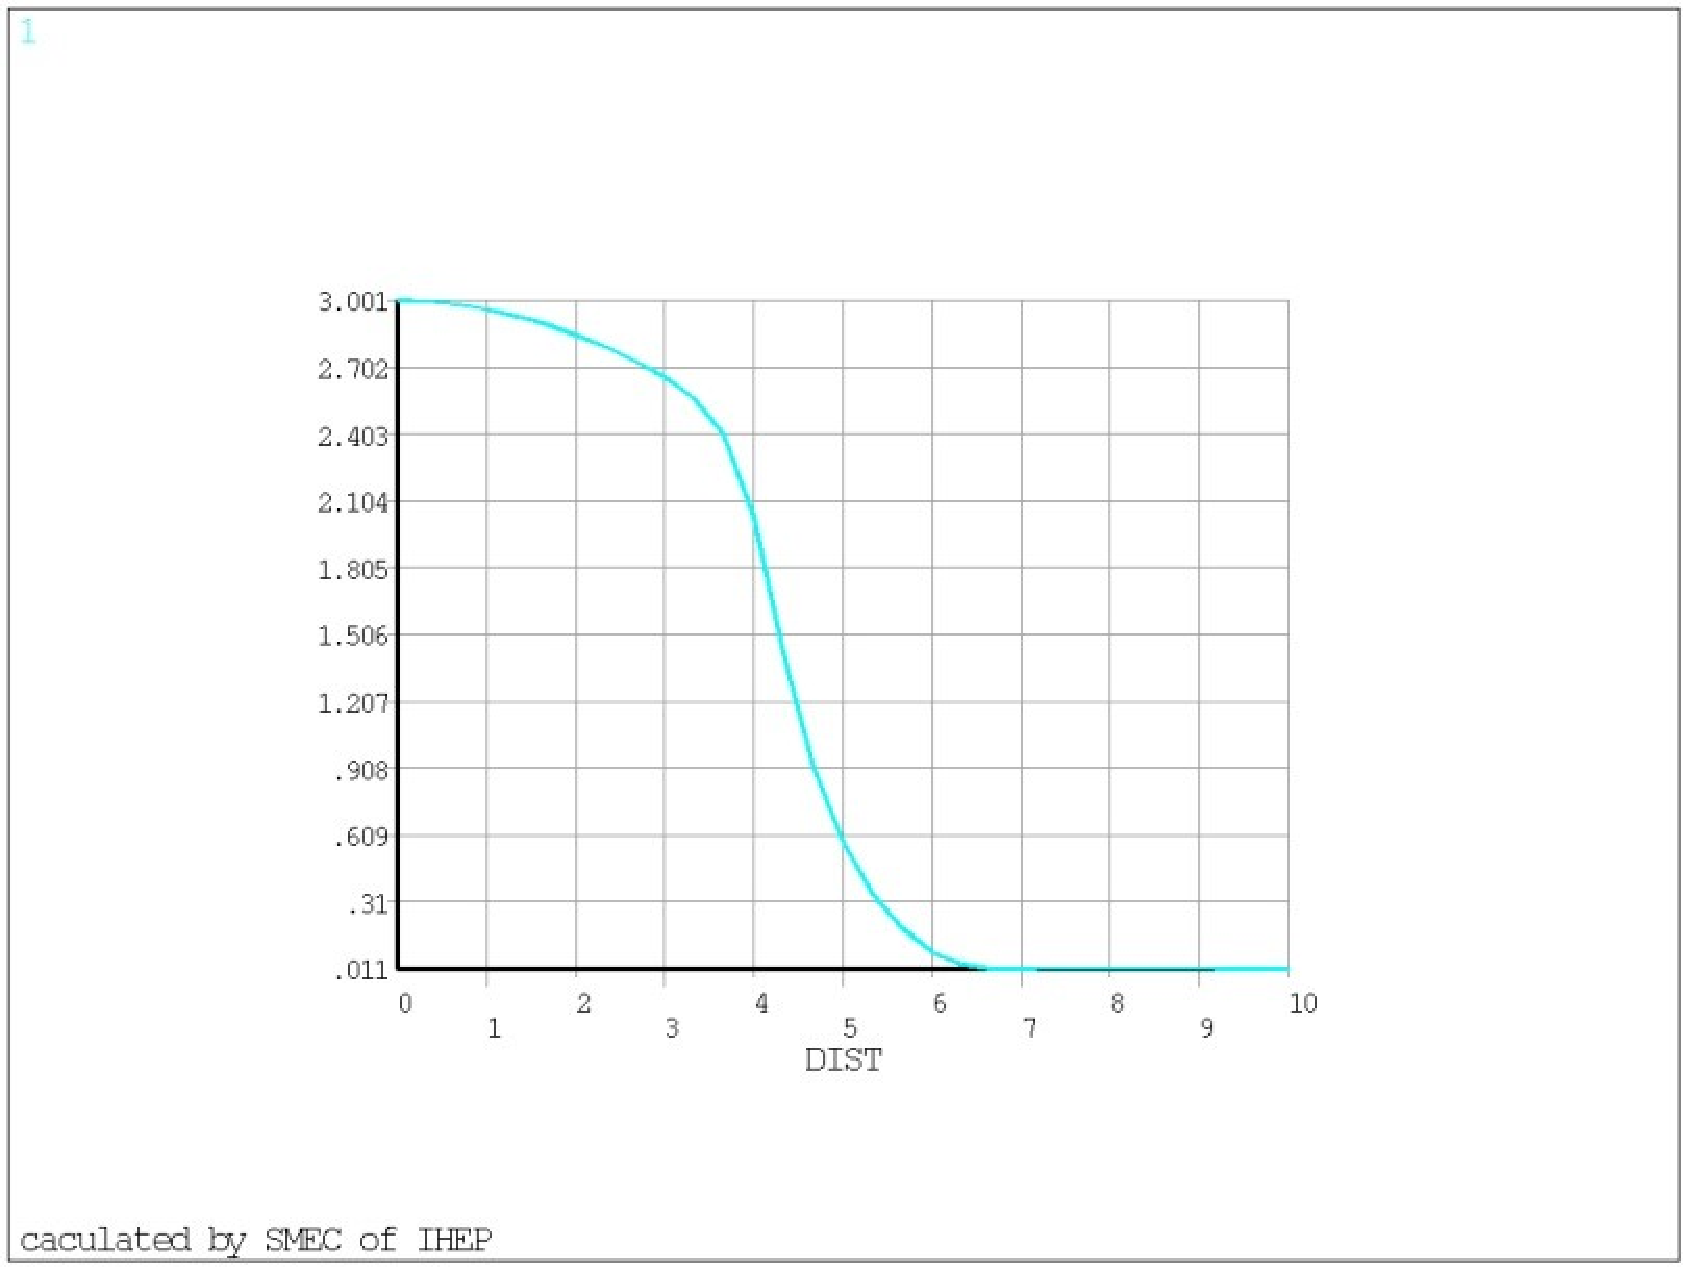
\includegraphics[scale=0.36]{Figures/Magnet/24}
\caption{The calculated magnetic field Bz along the detector axis}
\label{fig:24}
\end{figure}
%
\begin{figure}[h!]
\centering
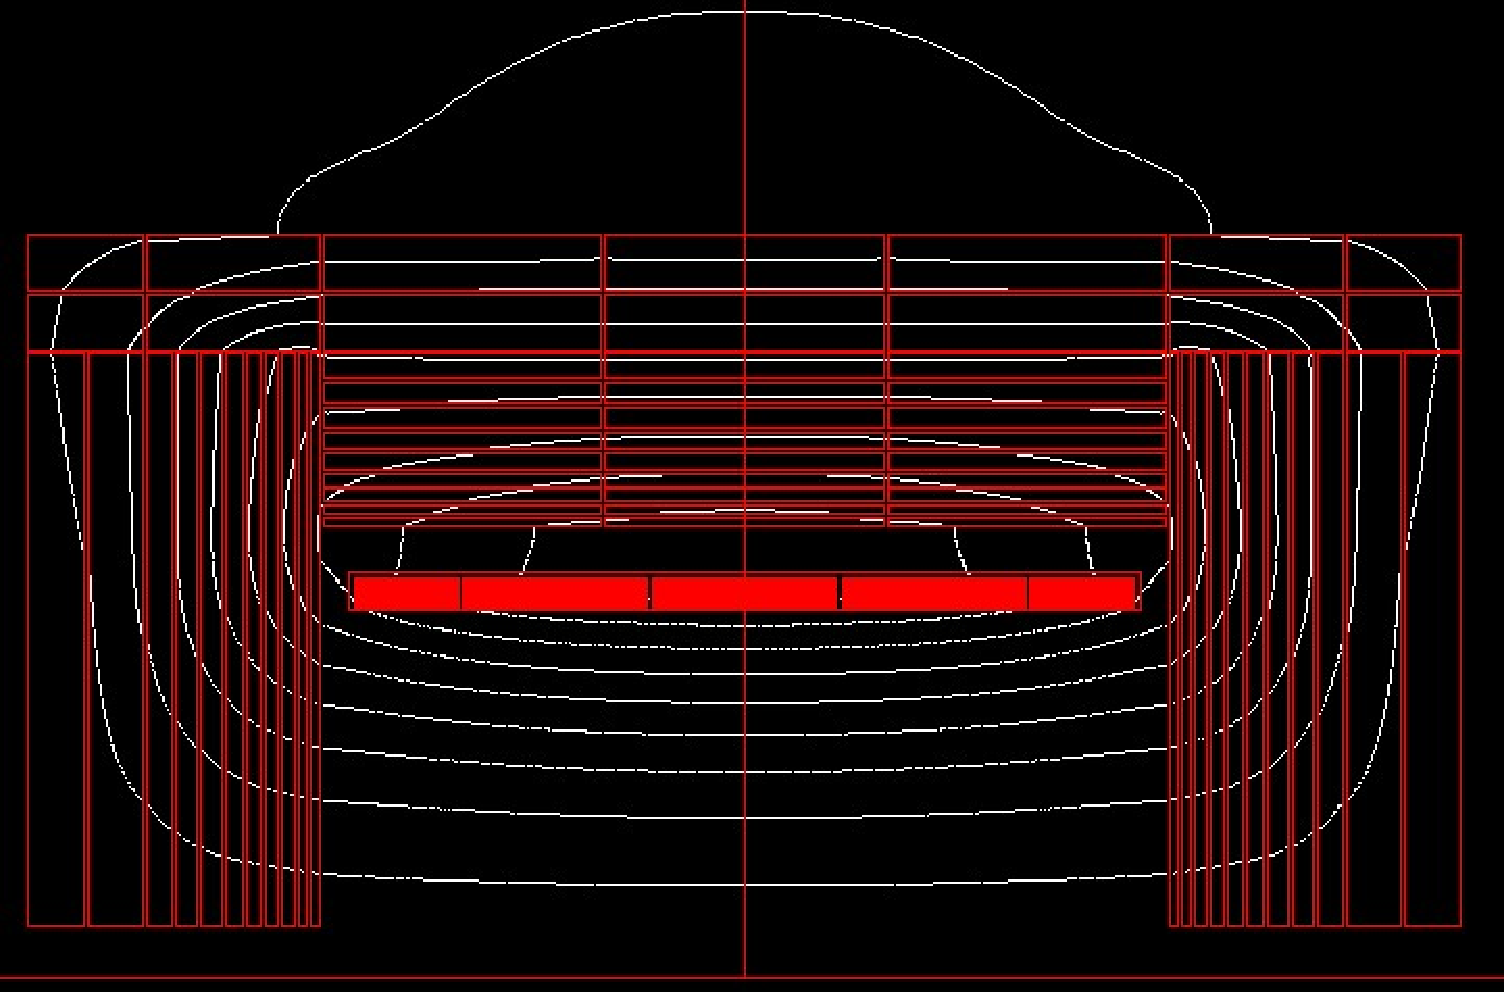
\includegraphics[scale=0.36]{Figures/Magnet/25}
\caption{Magnetic flux line distribution of the magnet}
\label{fig:25}
\end{figure}
%
\begin{figure}[h!]
\centering
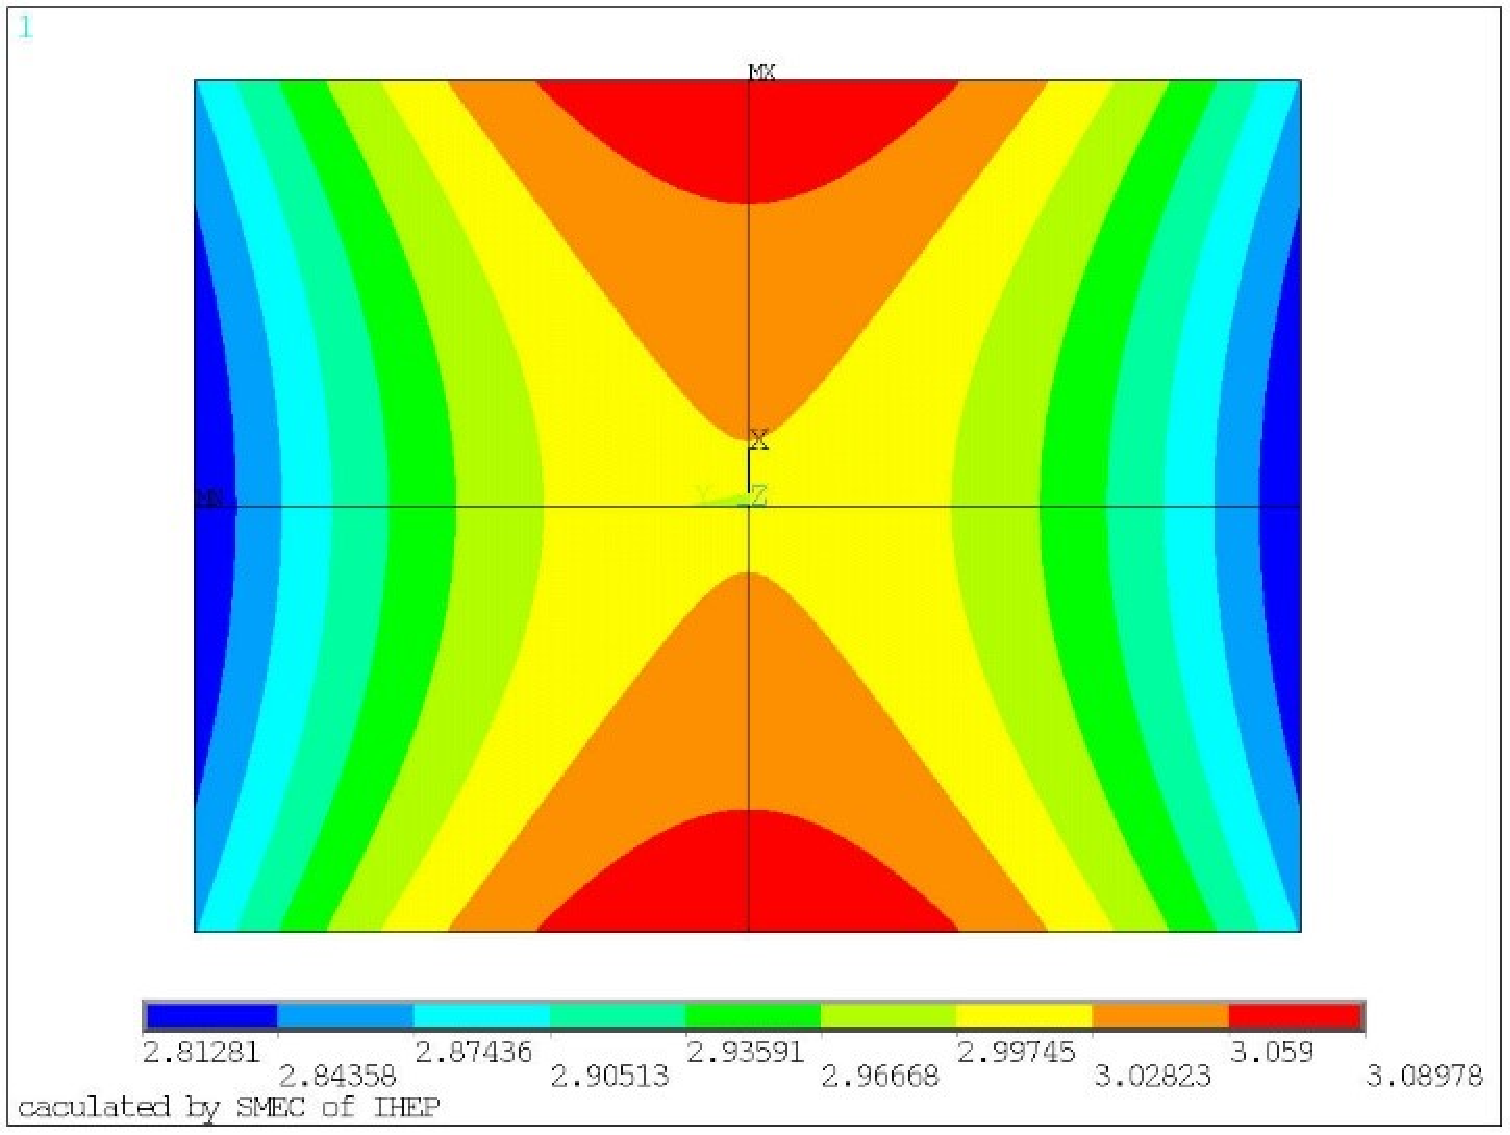
\includegraphics[scale=0.36]{Figures/Magnet/26}
\caption{The magnetic field distribution of TV}
\label{fig:26}
\end{figure}


The maximum magnetic field on the cable is 3.5 T on the pure aluminum stabilizer. This can be seen in Fig. 6.7 The magnetic field distribution on NbTi Rutherford cable is shown in Fig. 6.8. The maximum field on the NbTi cable is about 3.485 T. Fig. 6.9 shows the magnetic field distribution on the yoke.
%
\begin{figure}[h!]
\centering
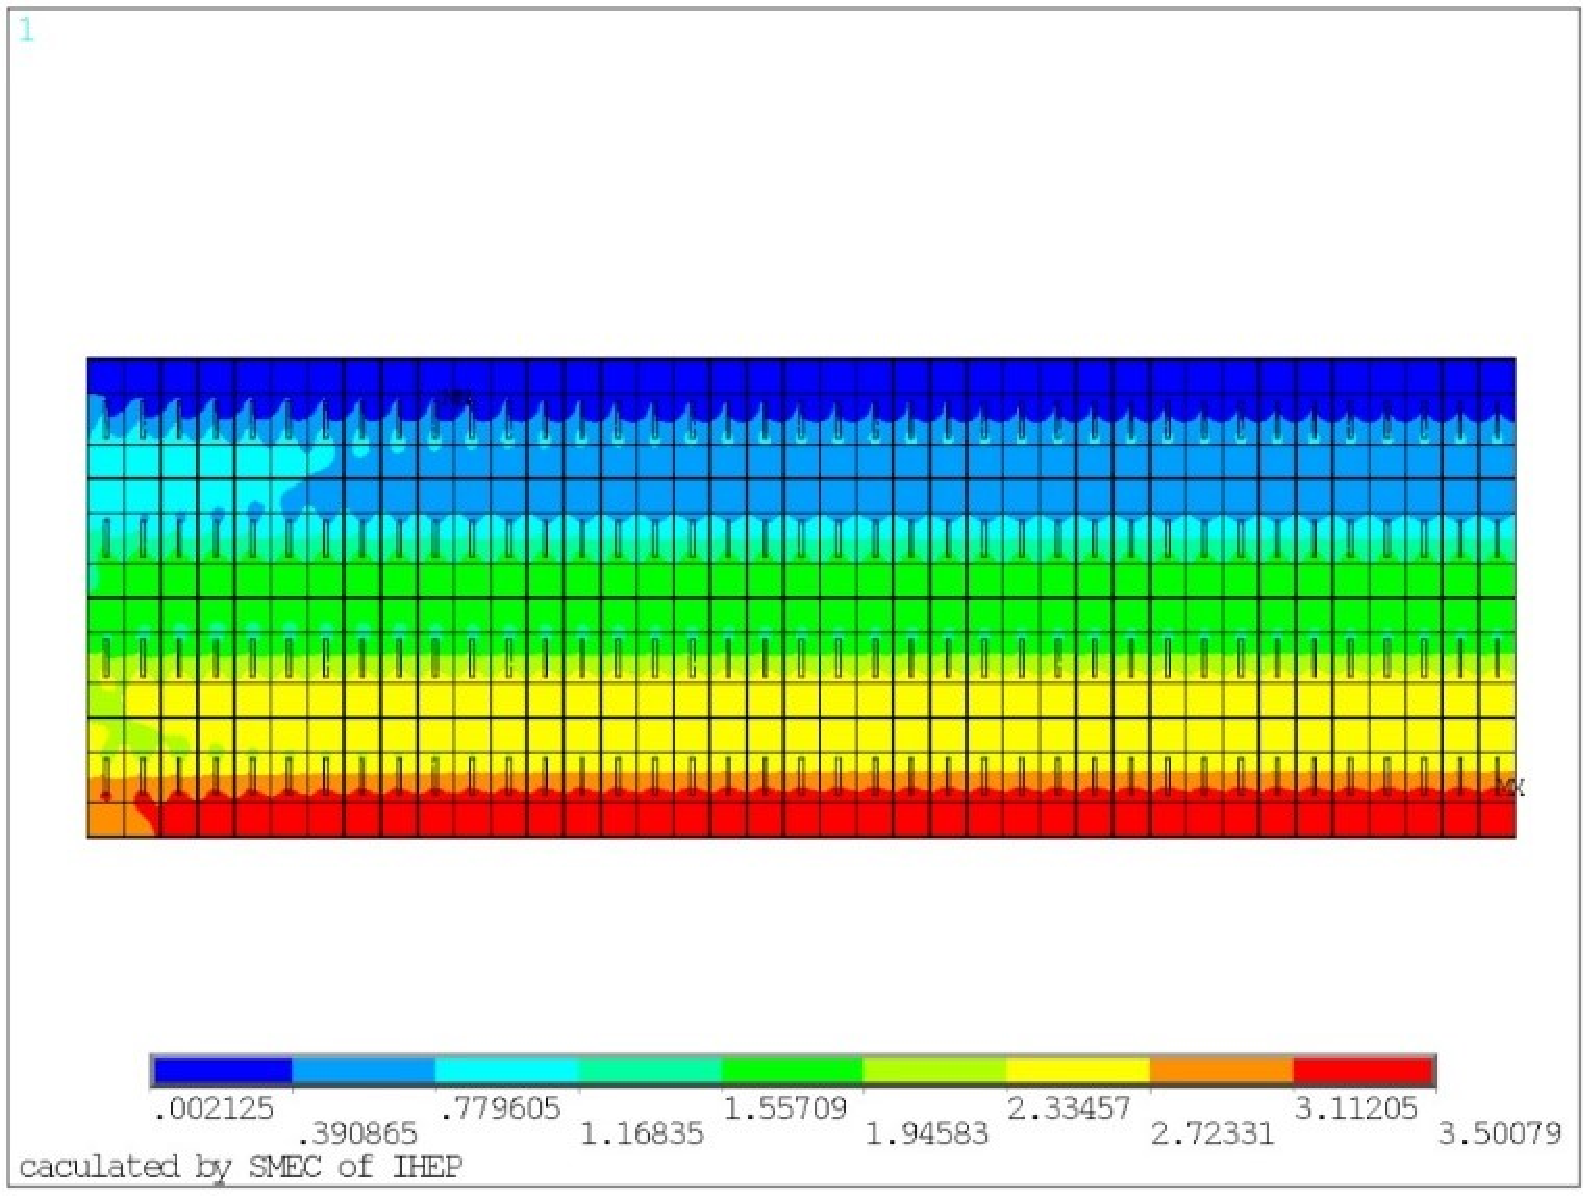
\includegraphics[scale=0.36]{Figures/Magnet/27}
\caption{Magnetic field distribution on the center model cable}
\label{fig:27}
\end{figure}
%
\begin{figure}[h!]
\centering
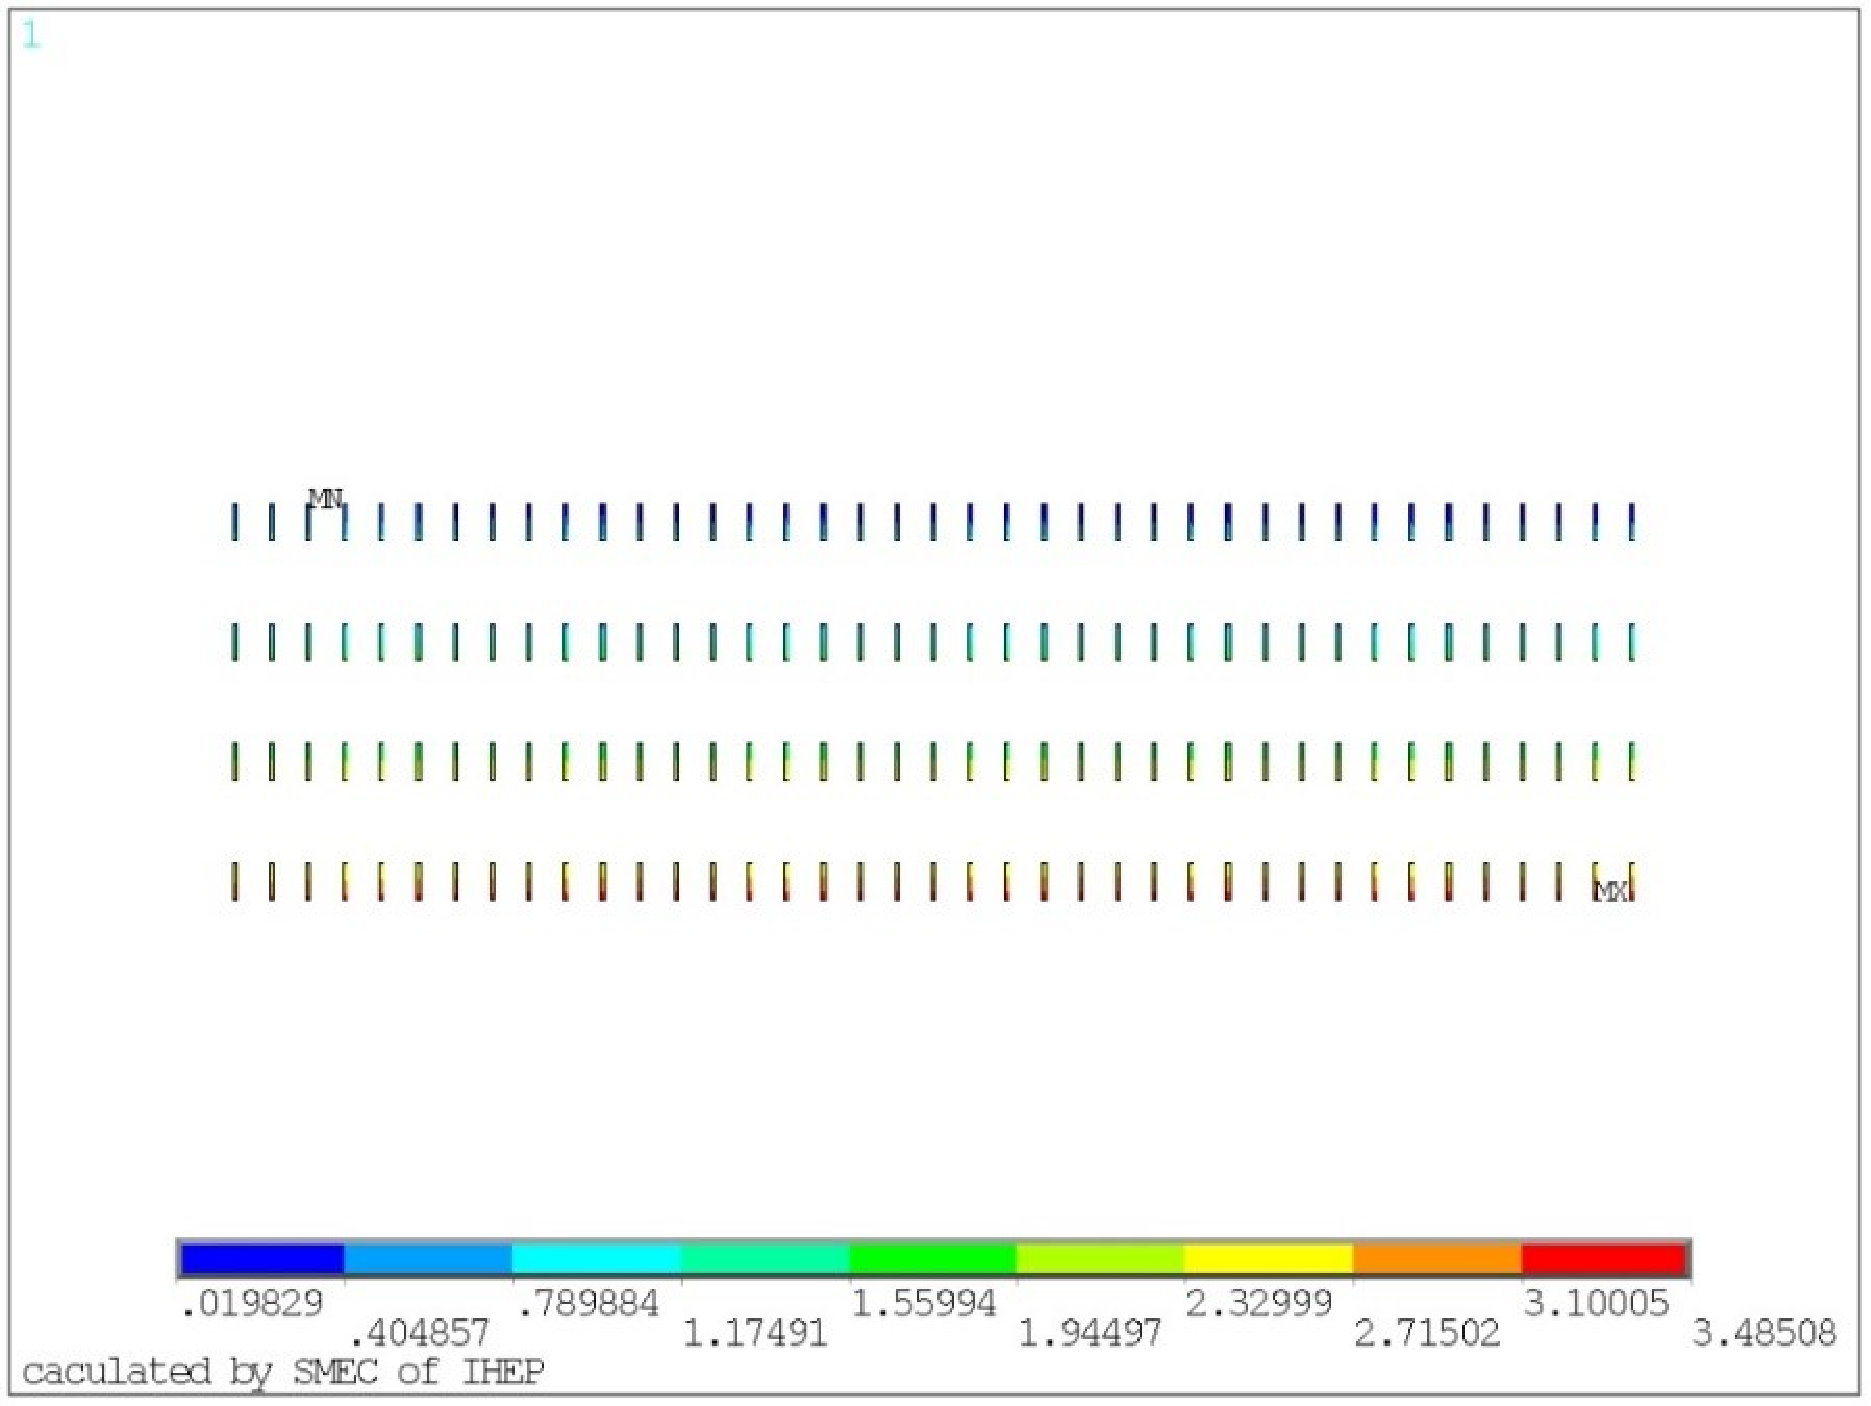
\includegraphics[scale=0.36]{Figures/Magnet/28}
\caption{Magnetic field distribution on the center NbTi cable}
\label{fig:28}
\end{figure}
%
\begin{figure}[h!]
\centering
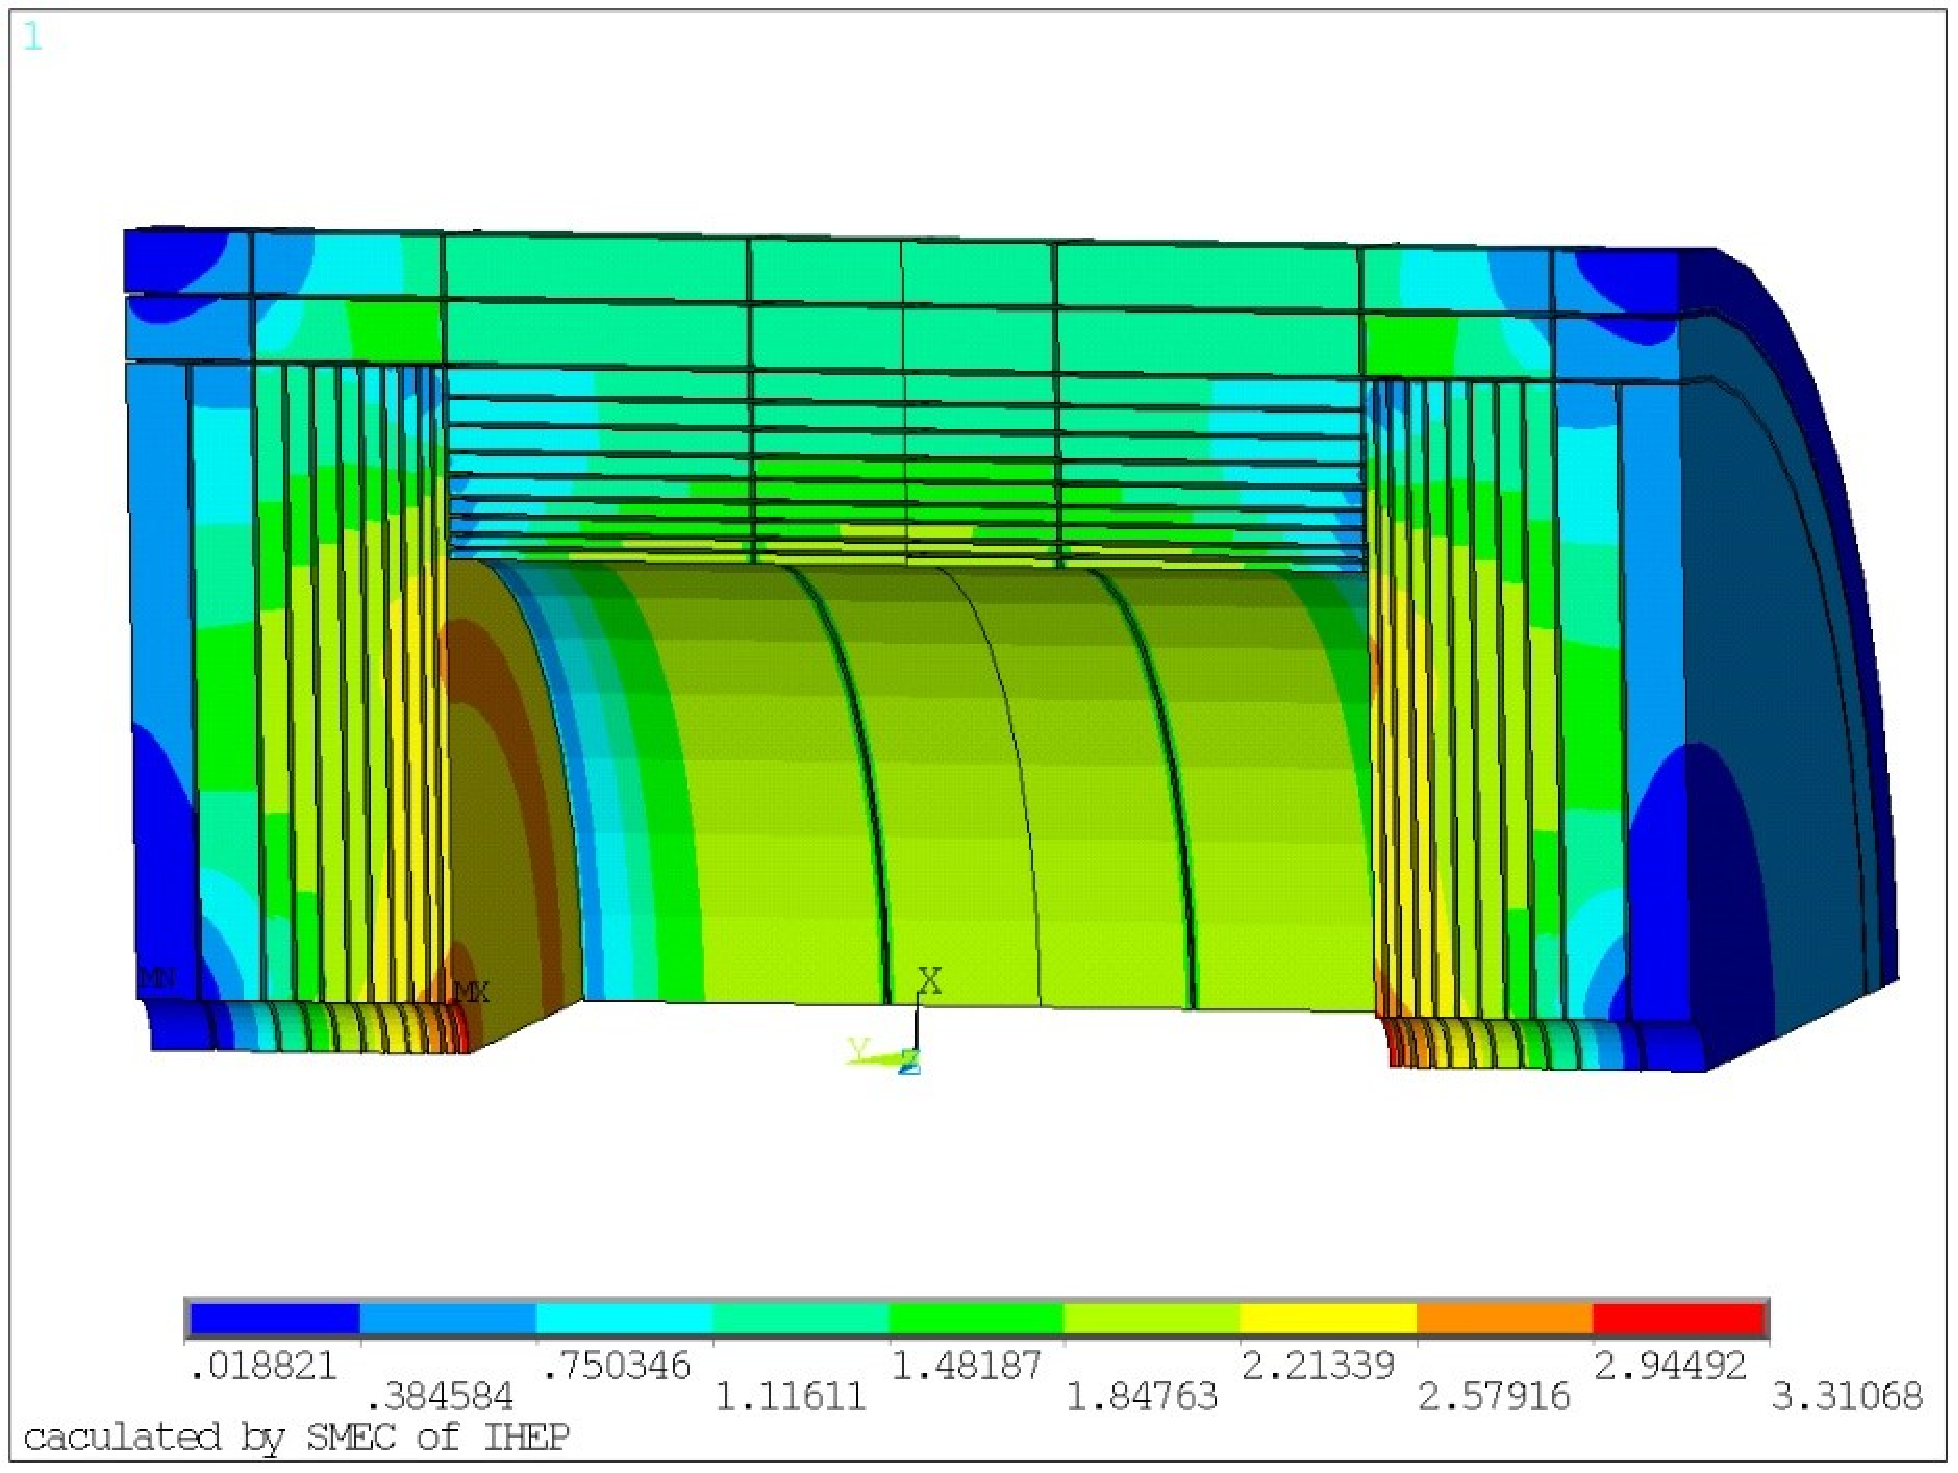
\includegraphics[scale=0.36]{Figures/Magnet/29}
\caption{Magnetic field distribution on the yoke}
\label{fig:29}
\end{figure}


The stray field of the detector magnet is show in Table 6.3 and Fig. 6.10. They give the stray field range of 50 Gs and 100 Gs.
\begin{table}[!h]
	\centering
	\begin{tabular}{c|c}
		\hline
		Stray field & 3 T \\
		\hline
		50Gs R direction & 13.6 m \\
		\hline
		50Gs Z direction & 15.8 m \\
		\hline
		100Gs R direction & 10 m \\
		\hline
		100Gs Z direction & 11.6 m \\
		\hline
	\end{tabular}
	\caption{ coil parameters}
	\label{tab:structure}
\end{table}
%
\begin{figure}[h!]
\centering
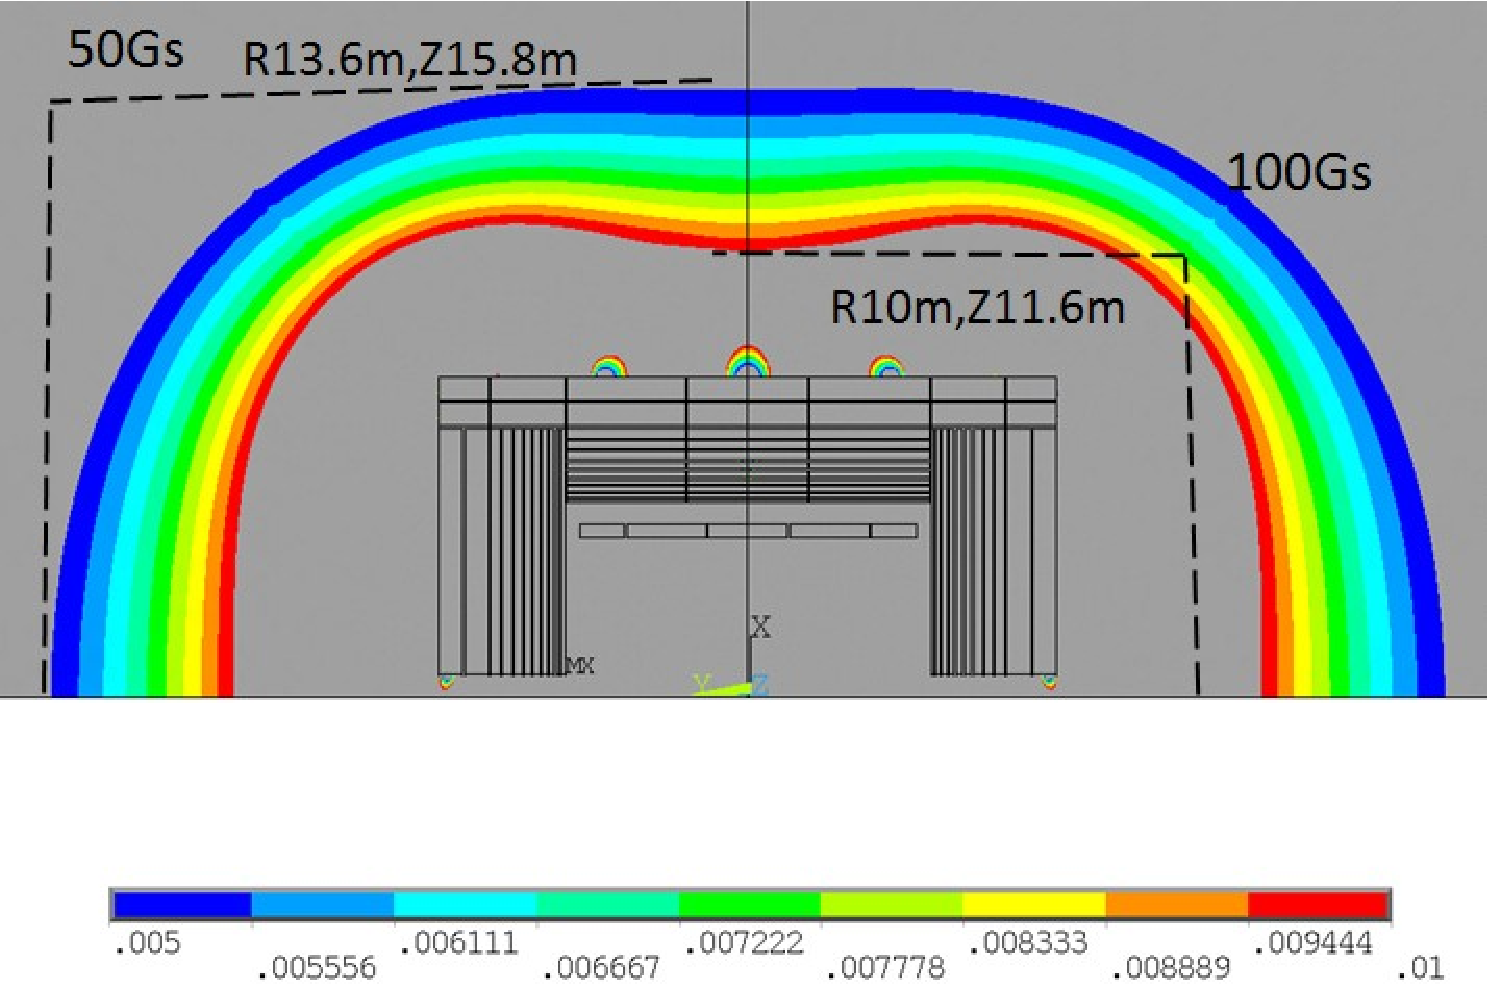
\includegraphics[scale=0.36]{Figures/Magnet/210}
\caption{Magnetic field distribution on the yoke}
\label{fig:210}
\end{figure}
\subsection{Coil mechanical analysis}
Introduction:


There are two kind of stress act on the coil: thermal mechanical force caused by inconsistent of the material expansion coefficient and magnetic force. The cable used is shown in Fig.6.2. The stress analysis is divided into two conditions: coil at 4.2 K; coil energized: 4.2 K, 15779 A, 3 T. A magnetic FEA was performed to calculate the thermal mechanical force and Lorentz force. 2-D axisymmetric mechanical analyses are carried out according to the coil. In the model there are some approximations have been made: the barrel yoke and end-cap yokes are transformed into cylinders; the hole of the chimney in the barrel has been neglected; the current (15779 A) in the winding has been modelled as uniformly distributed in the Rutherford cable. The thickness of the support is 50 mm, it��s the same with al-alloy used in the cable.
The properties of the different materials are given in Table 6.4 and Table 6.5. Table 6.4 gives the properties of every material used in the FEA. Table 6.5 shows mean integral thermal expansion coefficients used in the FEA.
\begin{table}[!h]
	\centering
	\begin{tabular}{c|c|c|c}
		\hline
		Material & Temperature(K) & Young��s Modulus (GPa) & Poisson��s ratio \\
		\hline
		Al & 4.2 & 0.8 & 0.49 \\
		\hline
		Al-Alloy & 4.2 & 77.7 & 0.327 \\
		\hline
		Sc strand & 4.2 & 130 & 0.3 \\
		\hline
		Fiber glass epoxy & 4.2 & 12.5 & 0.21 \\
		\hline
	\end{tabular}
	\caption{Material properties used in the FEA}
	\label{tab:structure}
\end{table}

\begin{table}[!h]
	\centering
	\begin{tabular}{c|c}
		\hline
		Material & Mean integral thermal expansion coefficient 293K��4.2K \\
		\hline
		Aluminum & 14.23e-6 \\
		\hline
		Al-alloy & 14.16e-6 \\
		\hline
		Sc strand & 8.79e-6 \\
		\hline
		Fiber glass epoxy & 25.5e-6 \\
		\hline
	\end{tabular}
	\caption{ Mean integral thermal expansion coefficients used in the FEA}
	\label{tab:structure}
\end{table}
The mechanical FE model:


The coil has been simulated with an elasto-plastic 2-D axisymmetric FE model. Fig.6.11 shows the coil with aligned turns. Different materials are shown with different colors. Fig.6.12 shows the mesh grid distribution of the model.
%
\begin{figure}[h!]
\centering
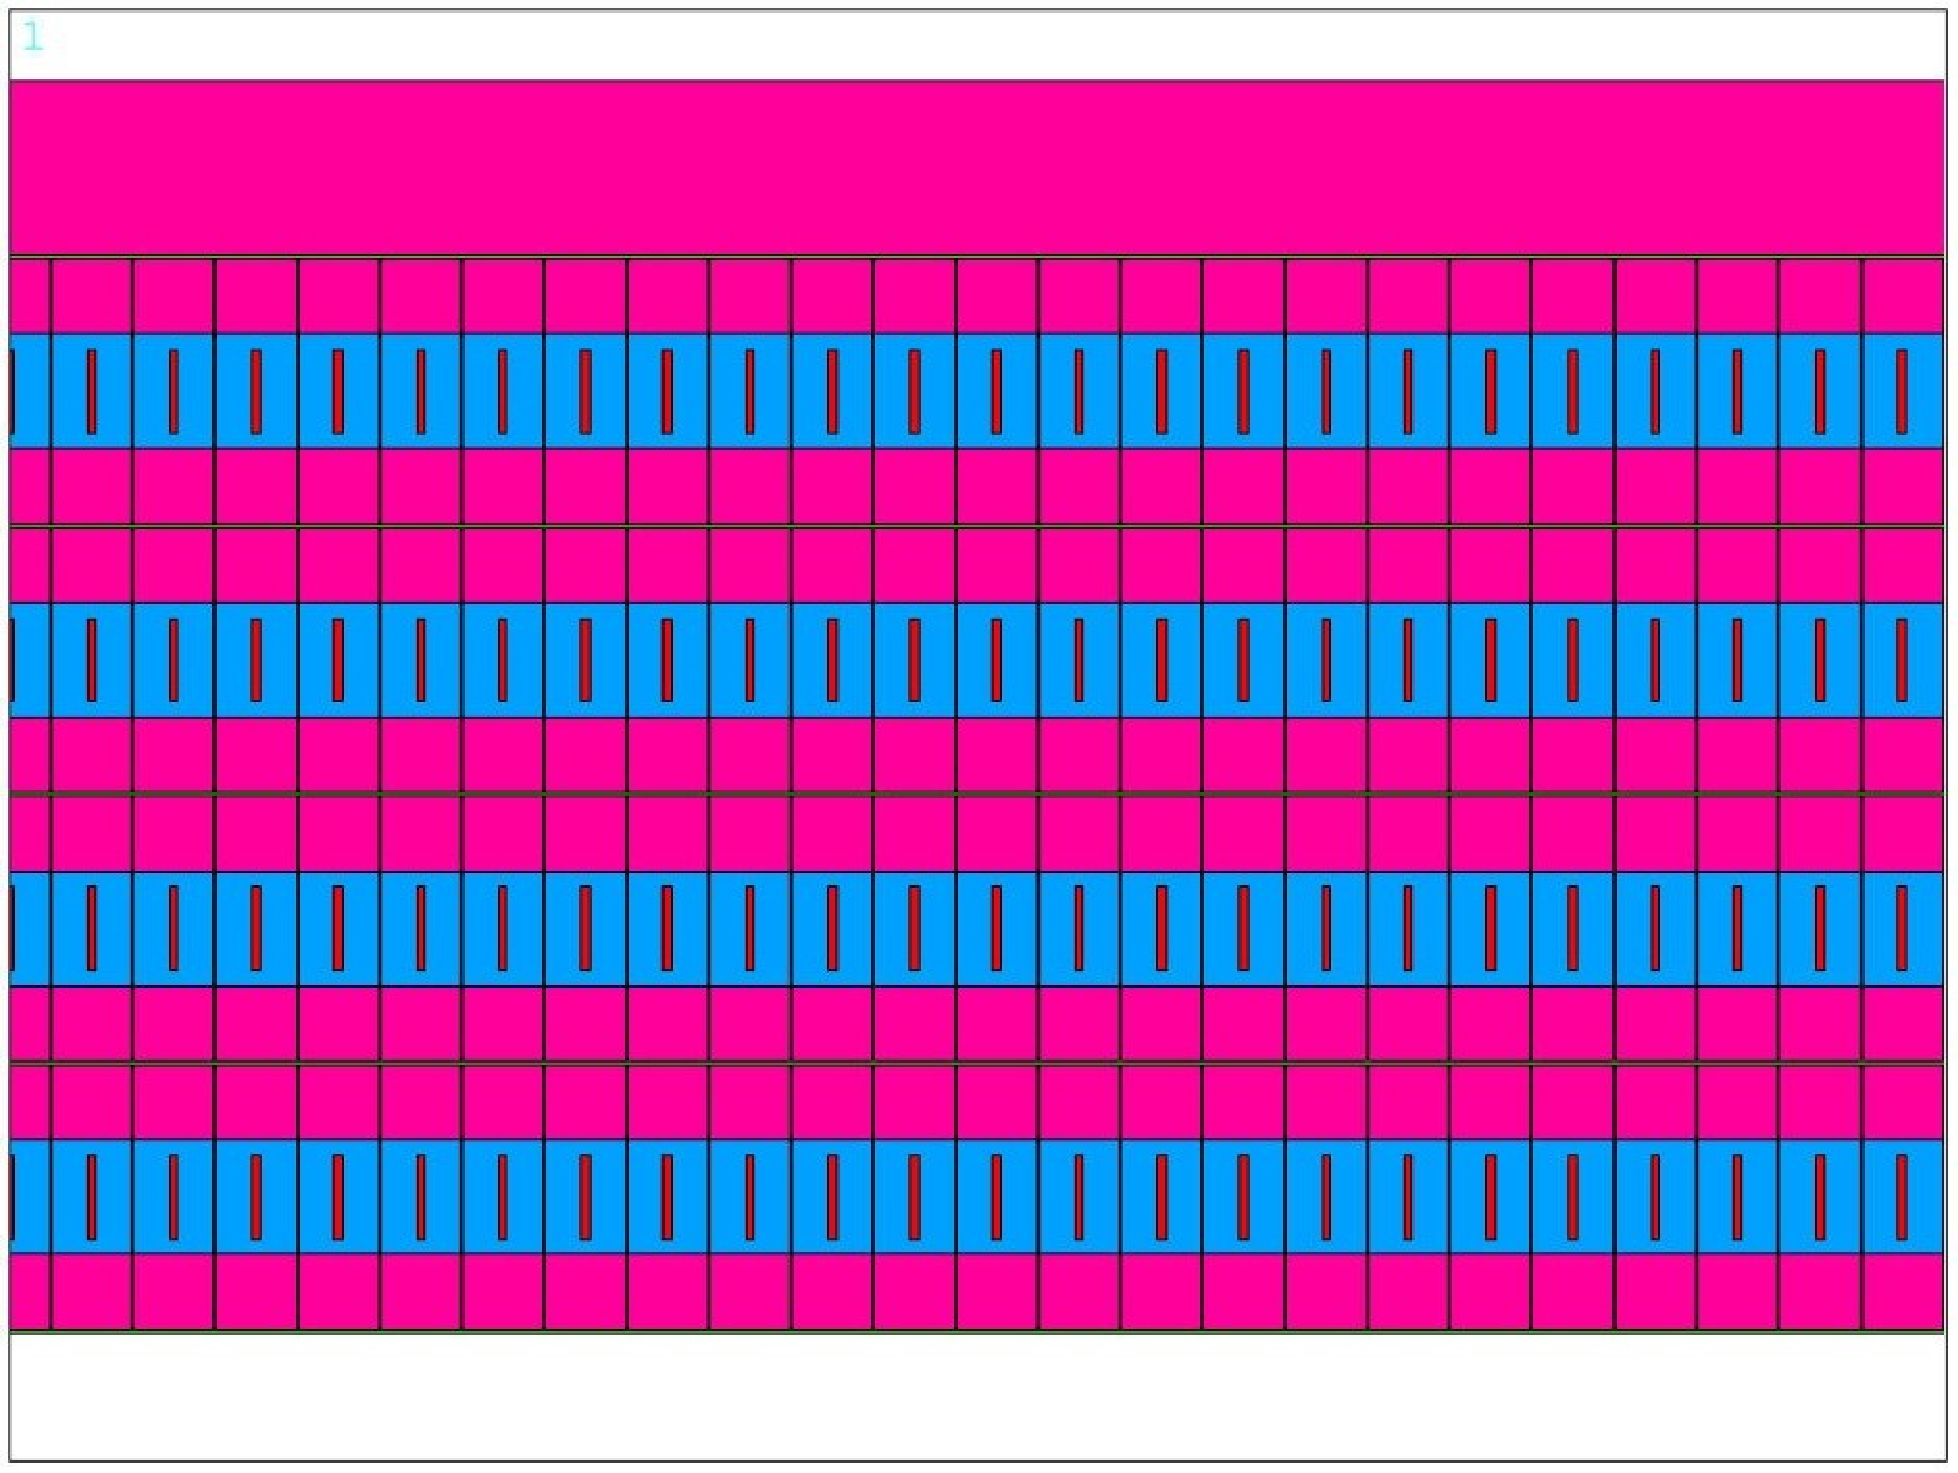
\includegraphics[scale=0.36]{Figures/Magnet/211}
\caption{Magnetic field distribution on the yoke}
\label{fig:212}
\end{figure}
Stress FEA results:


The Von Mises criterion has been used for all ductile materials present in the winding. A summary of the results is given in Table 6.6 and Table 6.7. From Fig.6.13 to Fig. 6.18 show the Von Mises of every part of coil when in the load cases of the coil at 4.2 K and energized. It seems that cool down gives the largest contribution to the stress field in SC cable and aluminum alloy, the effect of magnetic force seems to be relatively small.
\begin{table}[!h]
	\centering
	\begin{tabular}{c|p{4cm}|p{4cm}|p{4cm}}
		\hline
		Material & Von Mises stress MPa End coil & Von Mises stress MPa Middle coil & Von Mises stress MPa Central coil \\
		\hline
		\multicolumn{4}{|c|}{Coil at 4.2 K} \\
		\hline
		Pure Aluminum & 0-7.2 & 0-6.8 & 0-7 \\
		\hline
		SC cable & 189-205 & 190-201 & 189-200 \\
		\hline
		Al alloy & 2.2-44 & 5-39 & 5-43 \\
		\hline
        \multicolumn{4}{|c|}{Coil at 4.2 K, energized} \\
		\hline
		Pure Aluminum & 0-9.3 & 0-8.5 & 0-9.3 \\
		\hline
		SC cable & 85-142 & 62-95 & 66-106 \\
		\hline
		Al alloy & 40-94 & 74-103 & 65-103 \\
		\hline
	\end{tabular}
	\caption{ Maximum Von Mises of conductors}
	\label{tab:structure}
\end{table}
%
\begin{table}[!h]
	\centering
	\begin{tabular}{c|p{4cm}|p{4cm}|p{4cm}}
		\hline
		 & End coil & Middle coil & Central coil \\
		\hline
		\multicolumn{4}{|c|}{Coil at 4.2 K} \\
		\hline
		Von Mises(MPa) & 21-60 & 19-59 & 21-59 \\
		\hline
		Shear Stress(MPa) & 1.2 & 8.8 & 1.3 \\
		\hline
        \multicolumn{4}{|c|}{Coil at 4.2 K, energized} \\
		\hline
		Von Mises(MPa) & 29-85 & 30-84 & 29-79 \\
		\hline
		Shear Stress(MPa) & 12.4 & 9.0 & 13.1 \\
		\hline
	\end{tabular}
	\caption{ Shear stress and Von Mises of the insulation}
	\label{tab:structure}
\end{table}
%
\begin{figure}[h!]
\centering
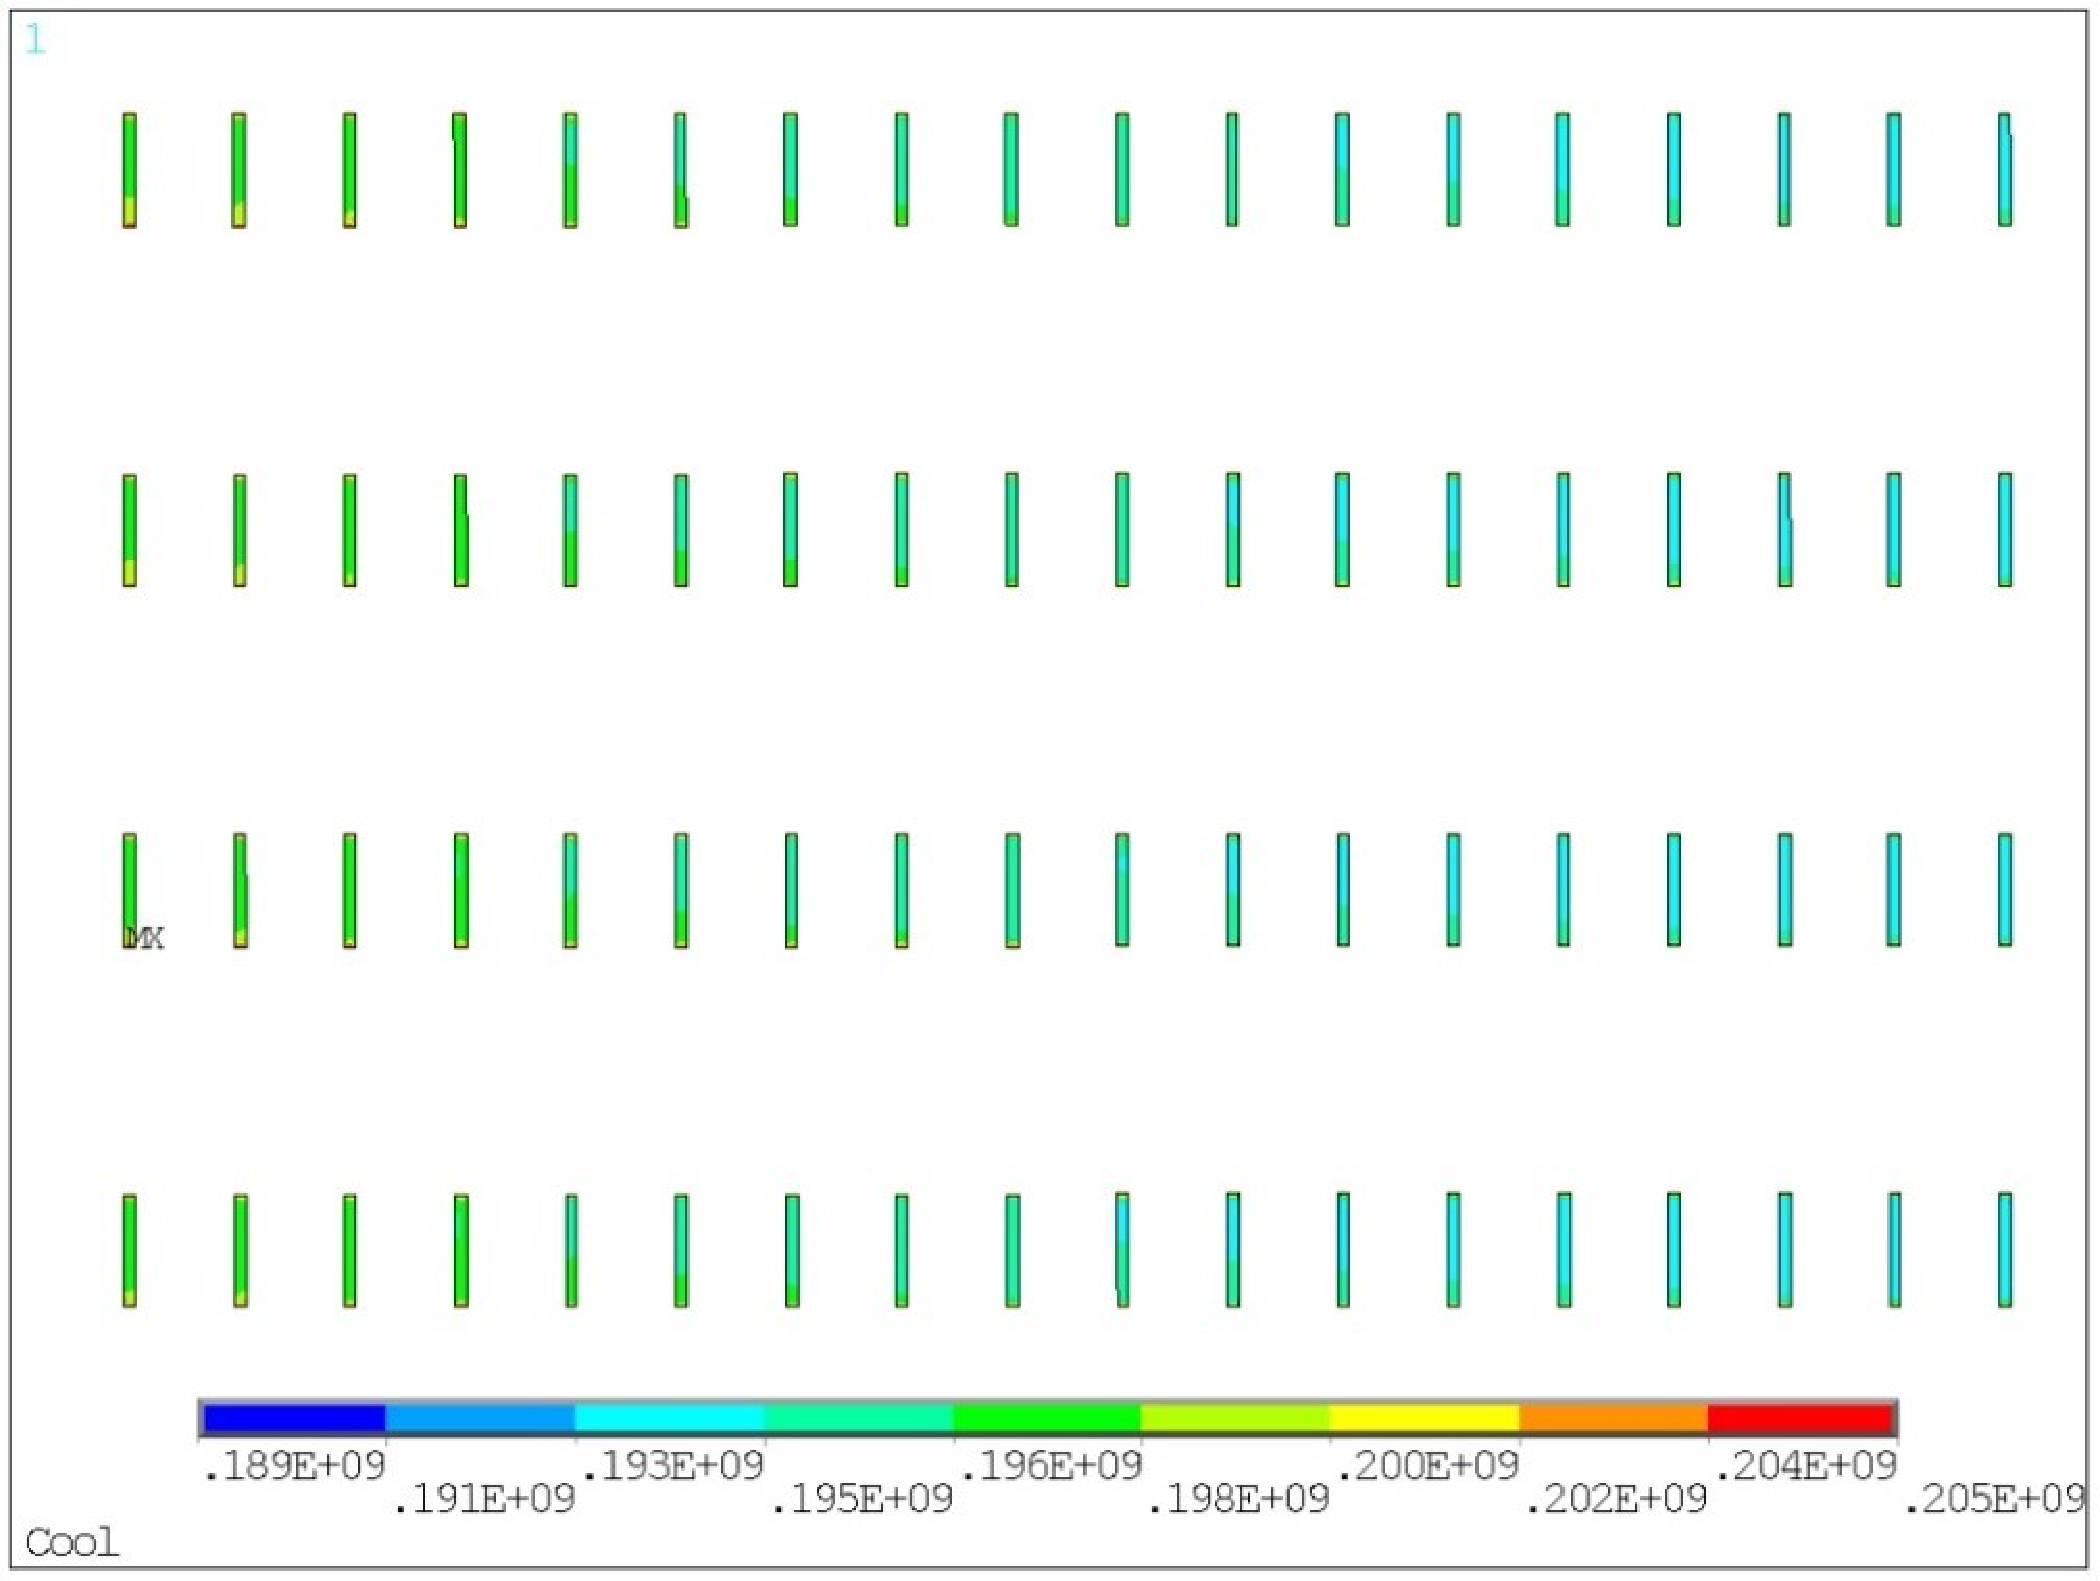
\includegraphics[scale=0.36]{Figures/Magnet/213}
\caption{Coil at 4.2 K, Von Mises distribution of the end coil SC cable}
\label{fig:213}
\end{figure}
%
\begin{figure}[h!]
\centering
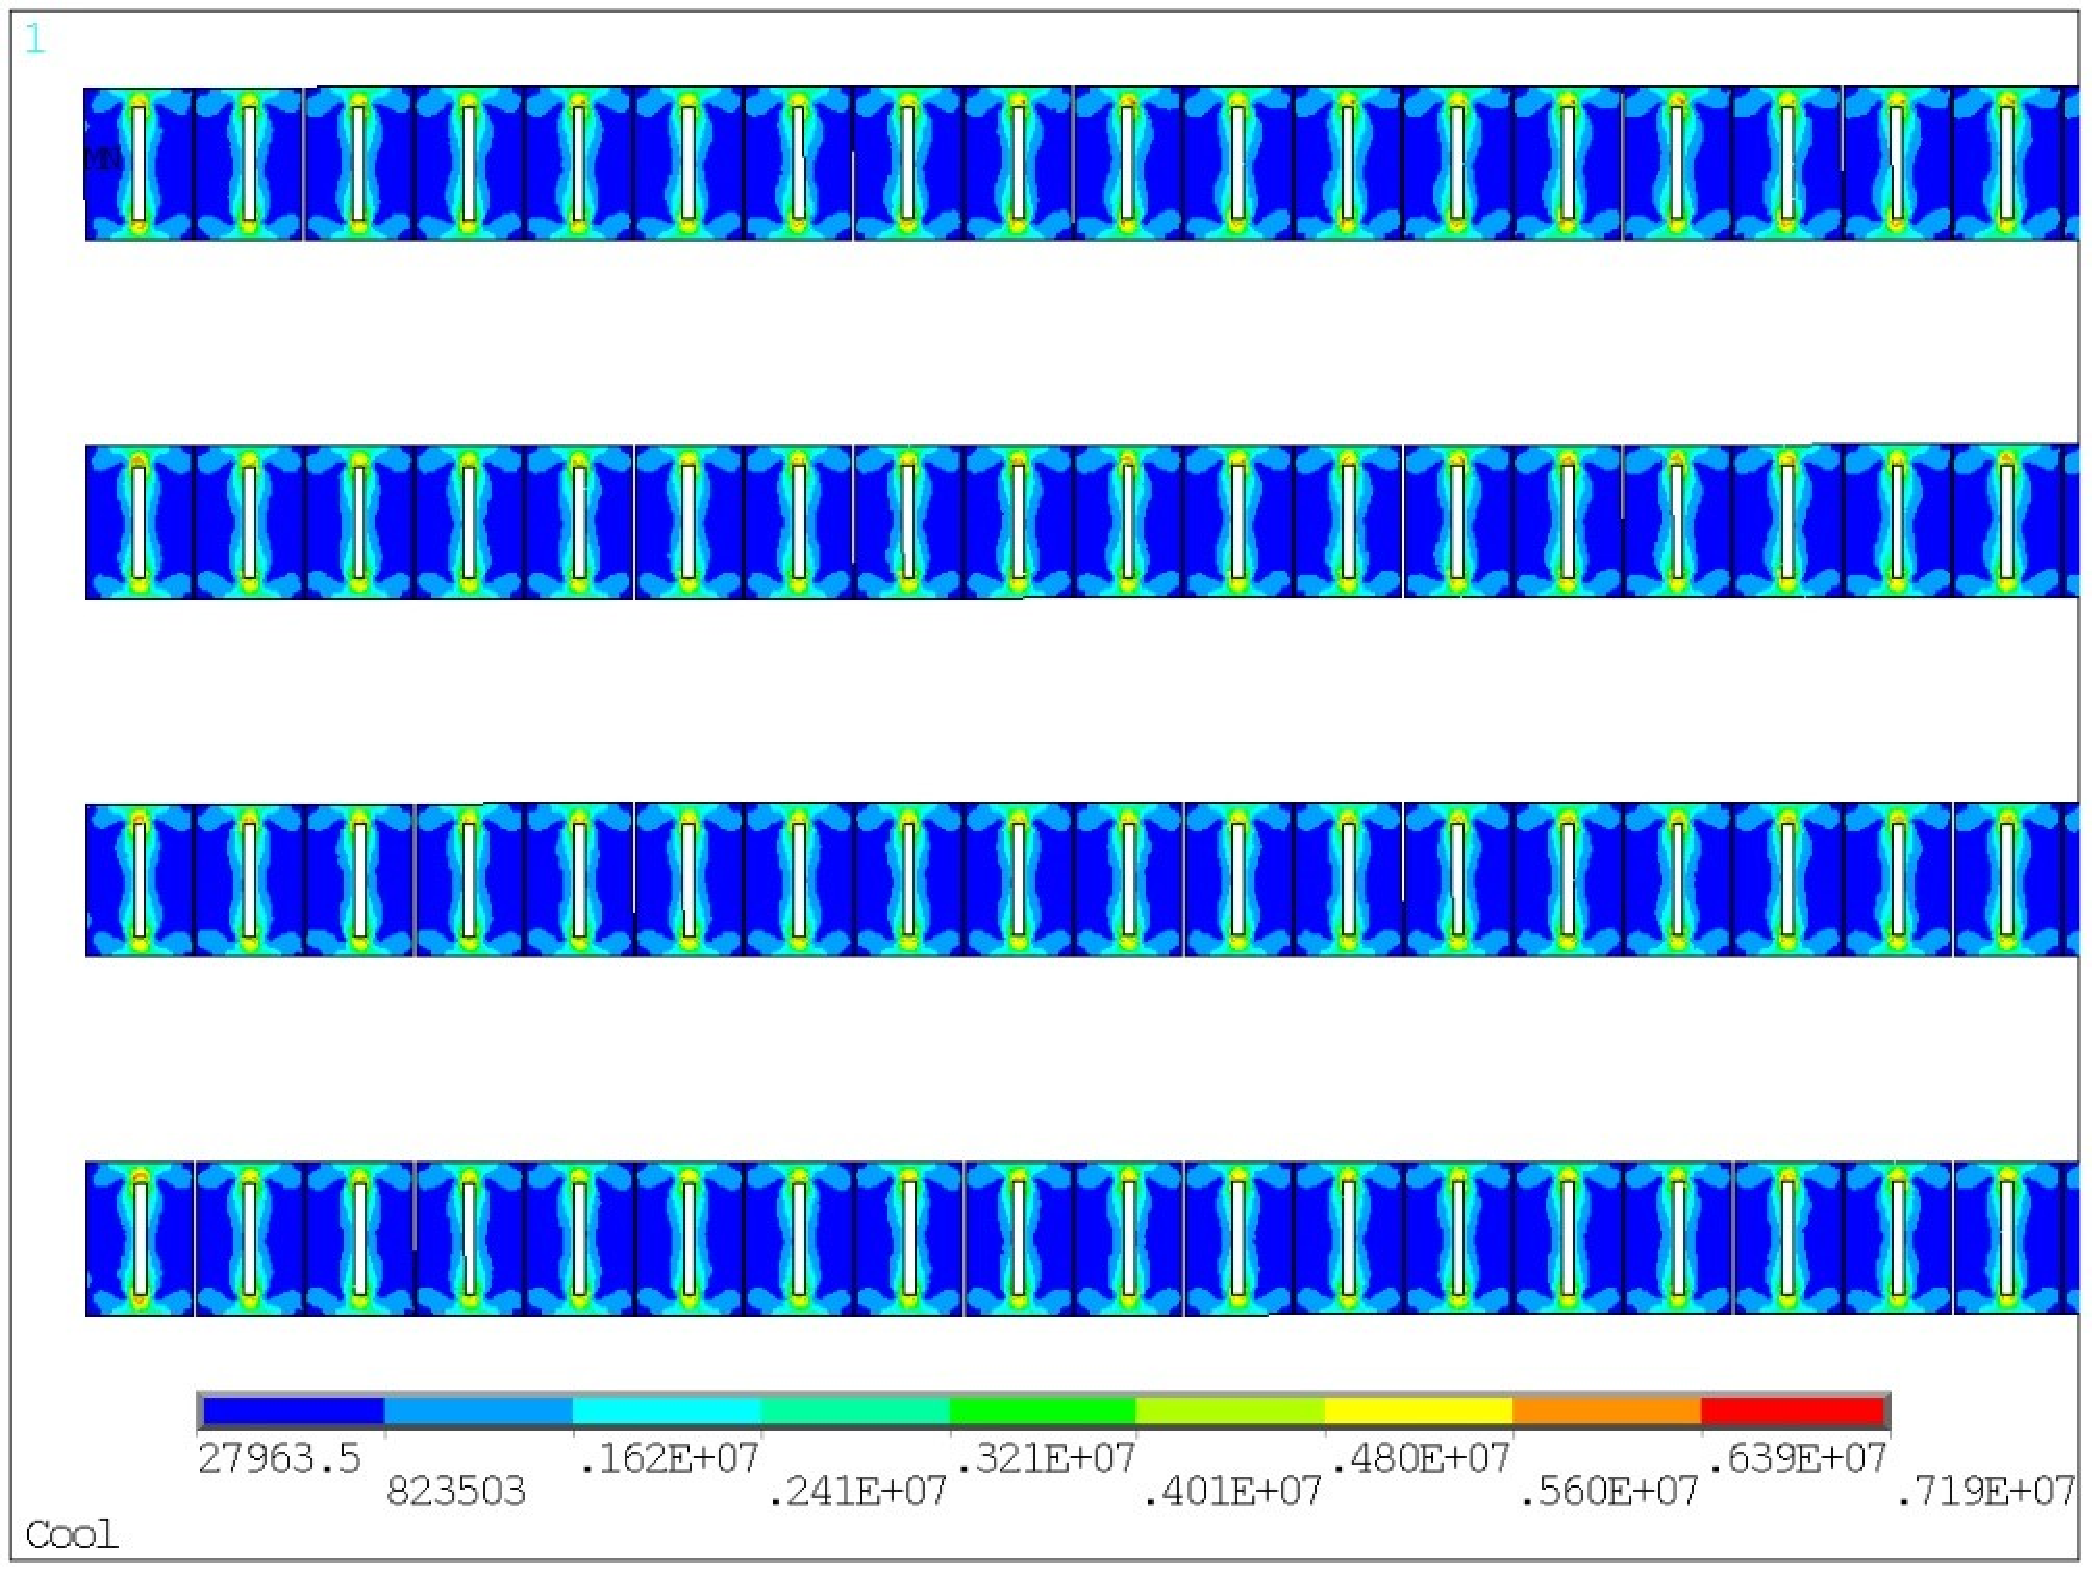
\includegraphics[scale=0.36]{Figures/Magnet/214}
\caption{Coil at 4.2 K, Von Mises distribution of the end coil pure Aluminum}
\label{fig:214}
\end{figure}
%
\begin{figure}[h!]
\centering
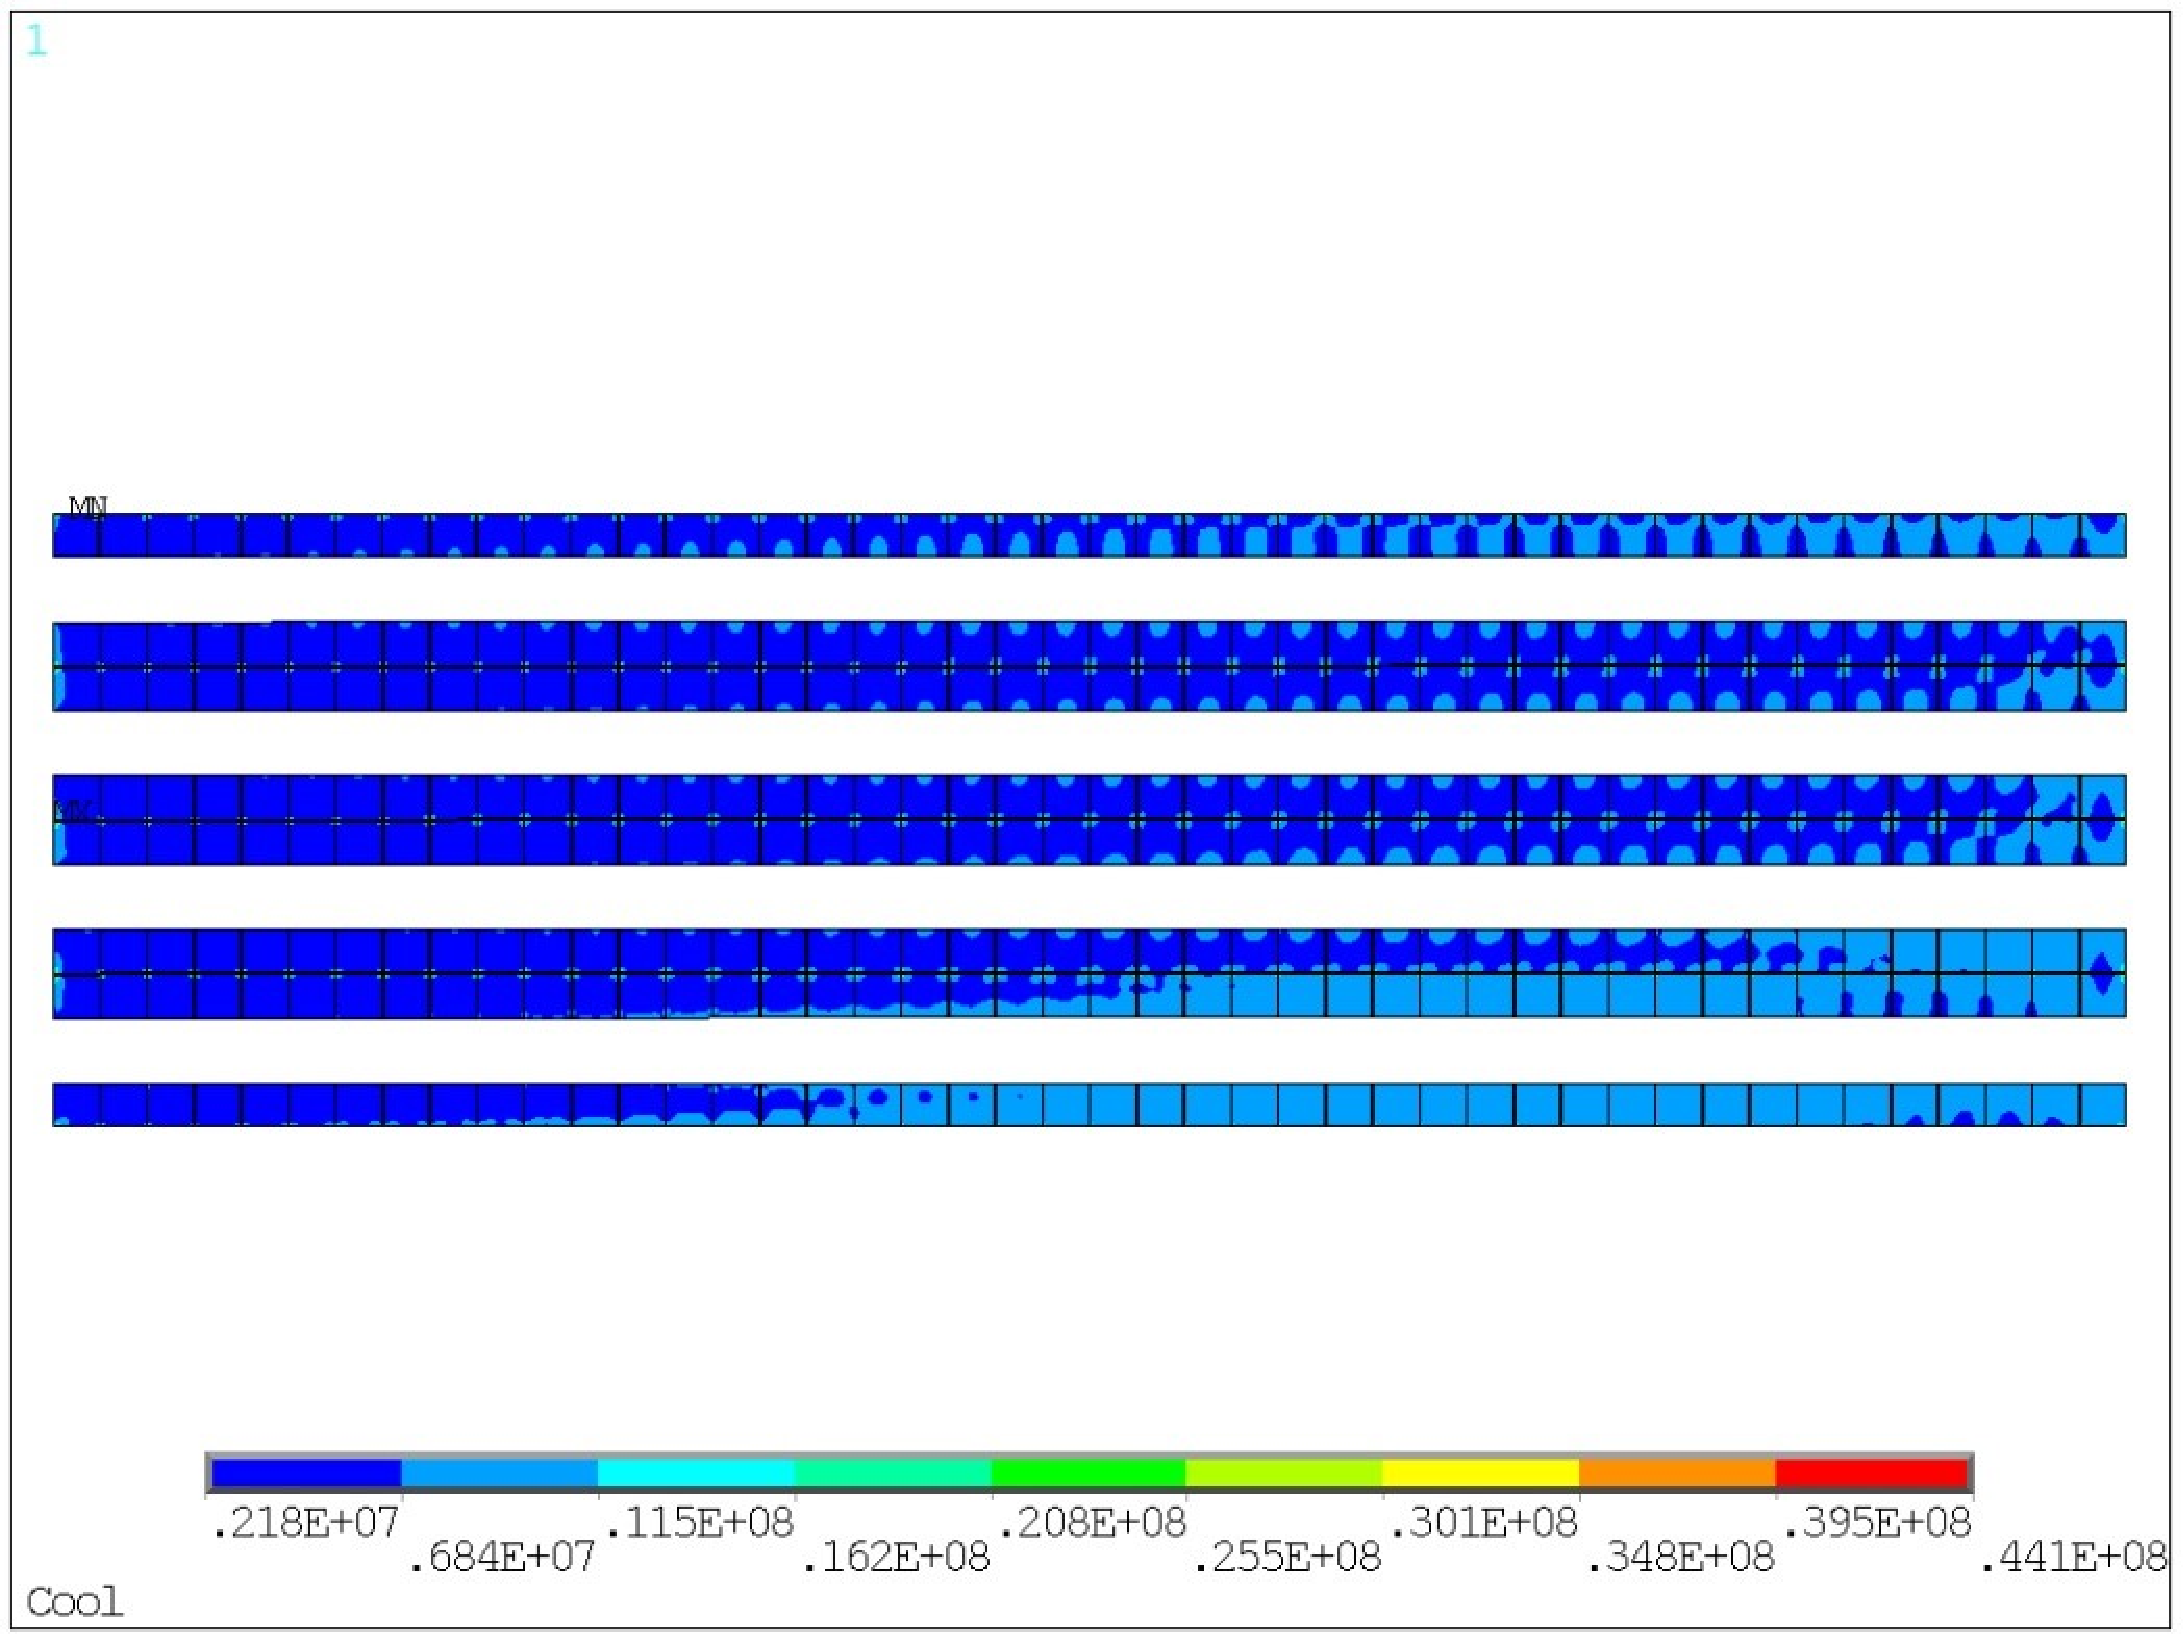
\includegraphics[scale=0.36]{Figures/Magnet/215}
\caption{ Coil at 4.2 K, Von Mises distribution of the end coil Aluminum alloy}
\label{fig:215}
\end{figure}
%
\begin{figure}[h!]
\centering
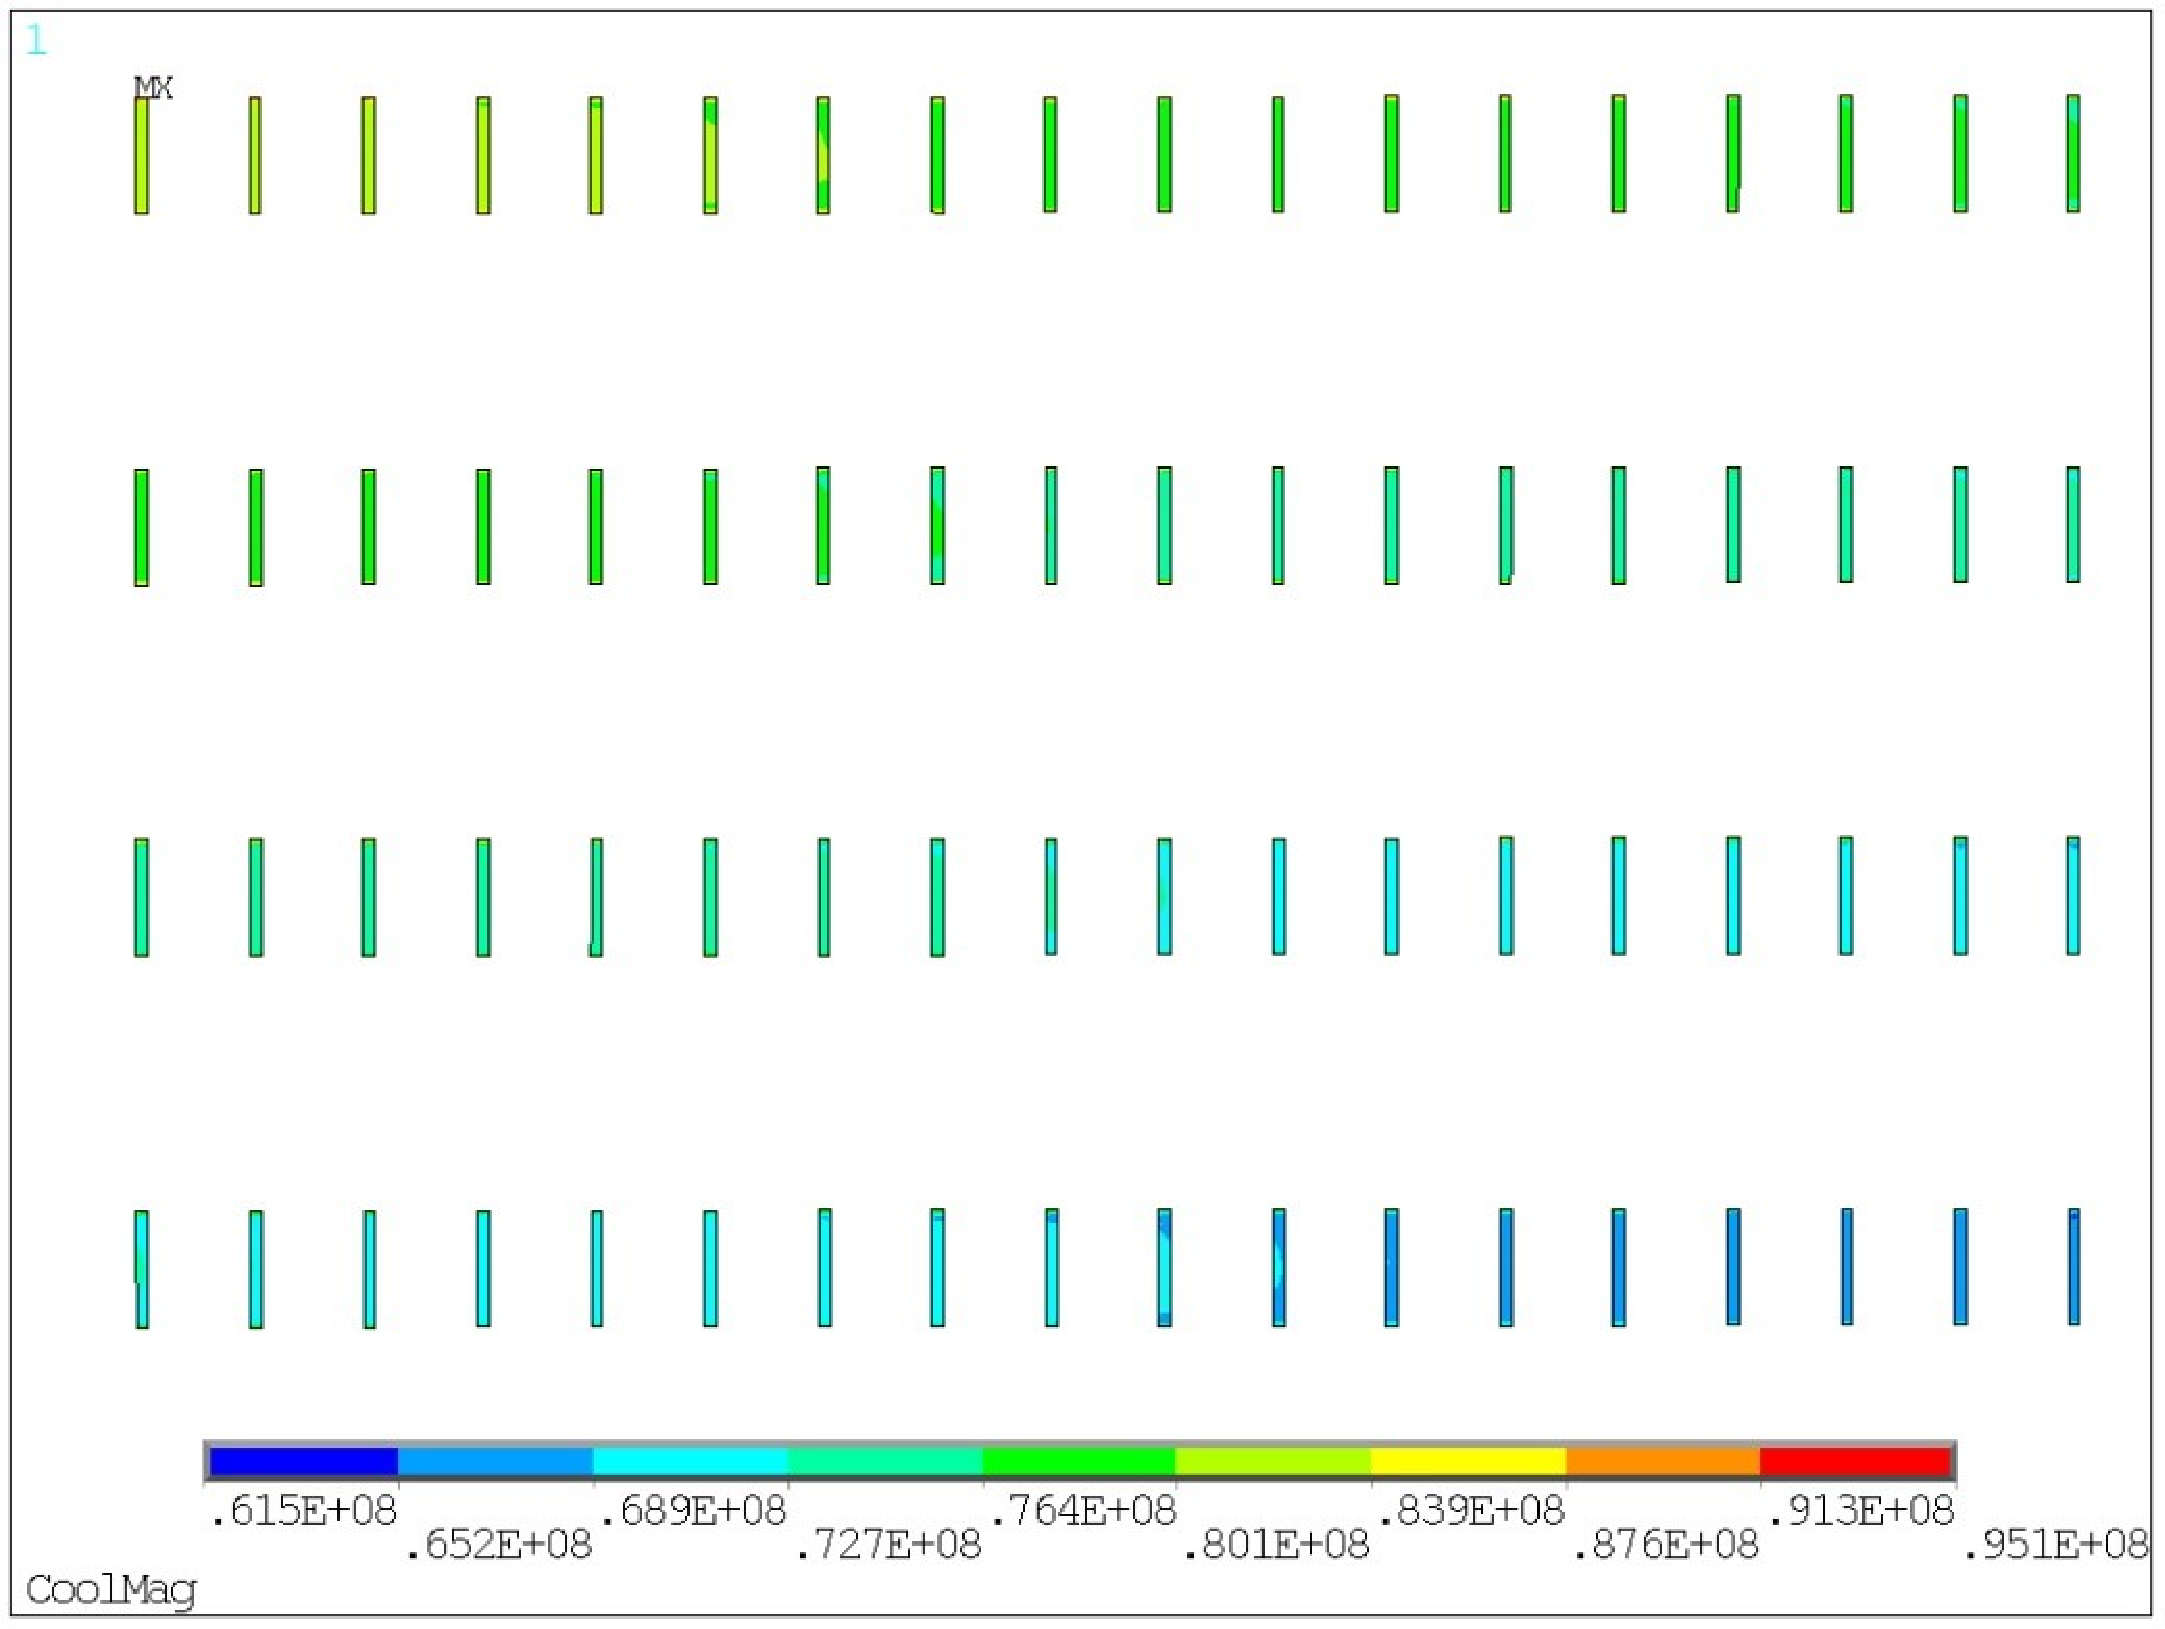
\includegraphics[scale=0.36]{Figures/Magnet/216}
\caption{ 6.16 Coil at 4.2 K, energized, Von Mises distribution of the central coil SC cable}
\label{fig:216}
\end{figure}
%
\begin{figure}[h!]
\centering
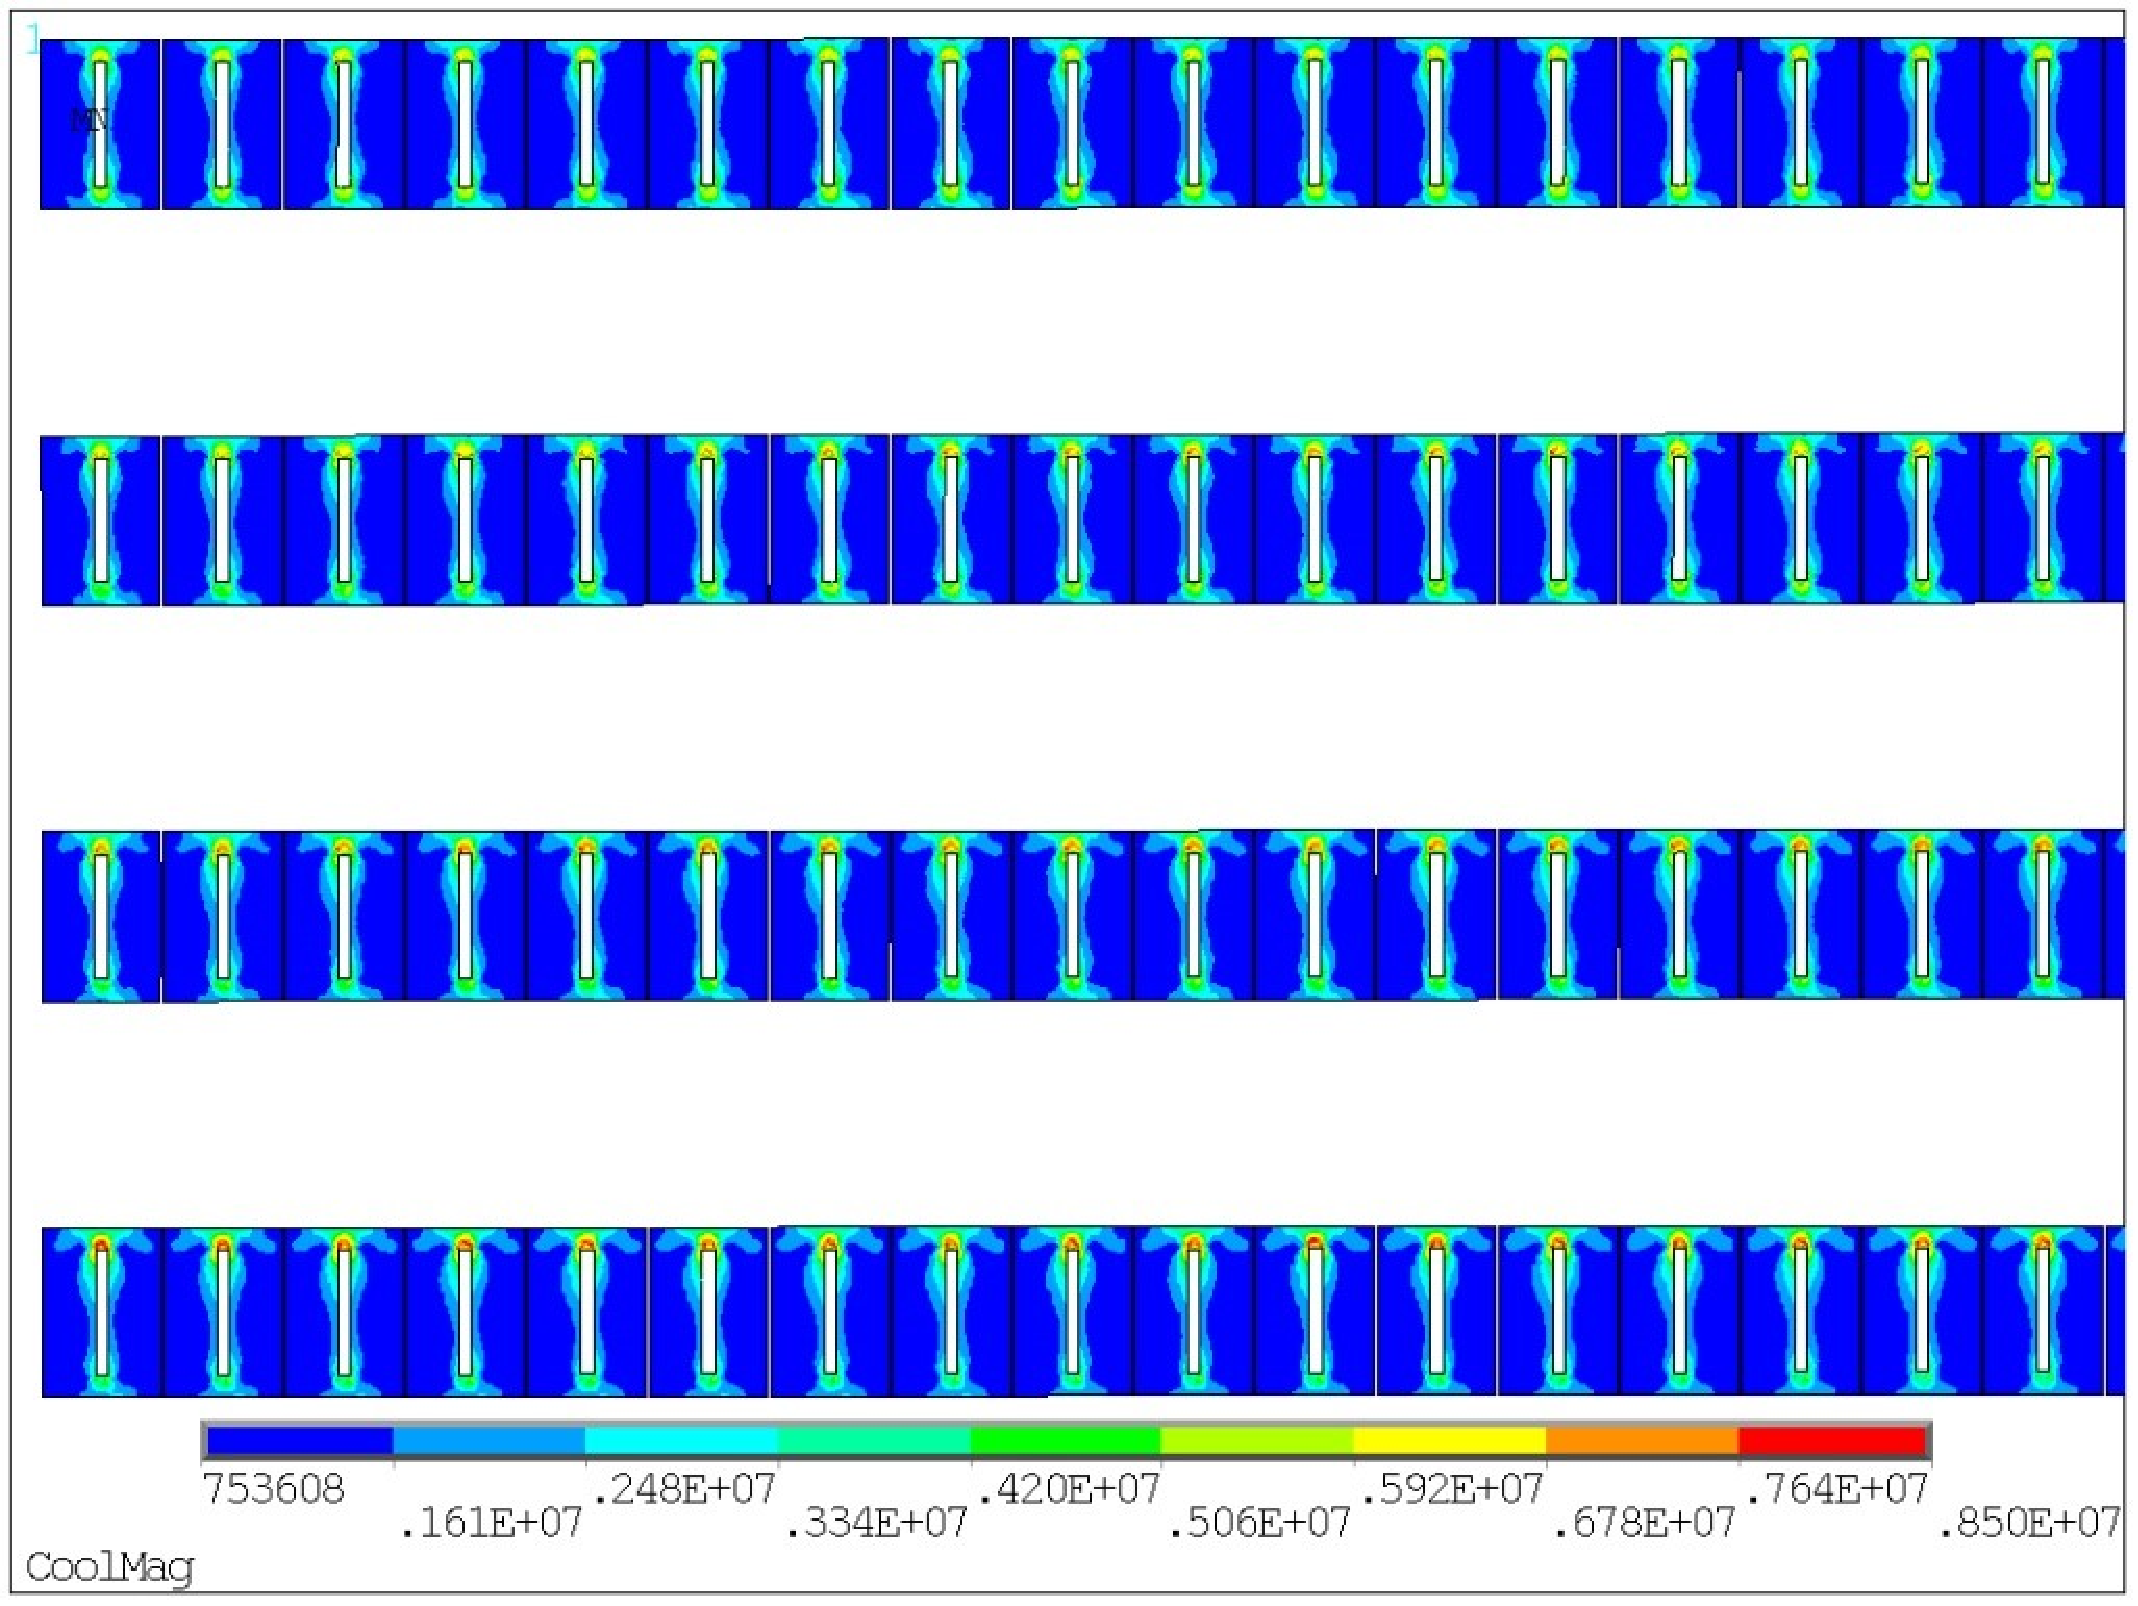
\includegraphics[scale=0.36]{Figures/Magnet/217}
\caption{Coil at 4.2 K, energized, Von Mises distribution of the central coil pure Aluminum}
\label{fig:217}
\end{figure}
%
\begin{figure}[h!]
\centering
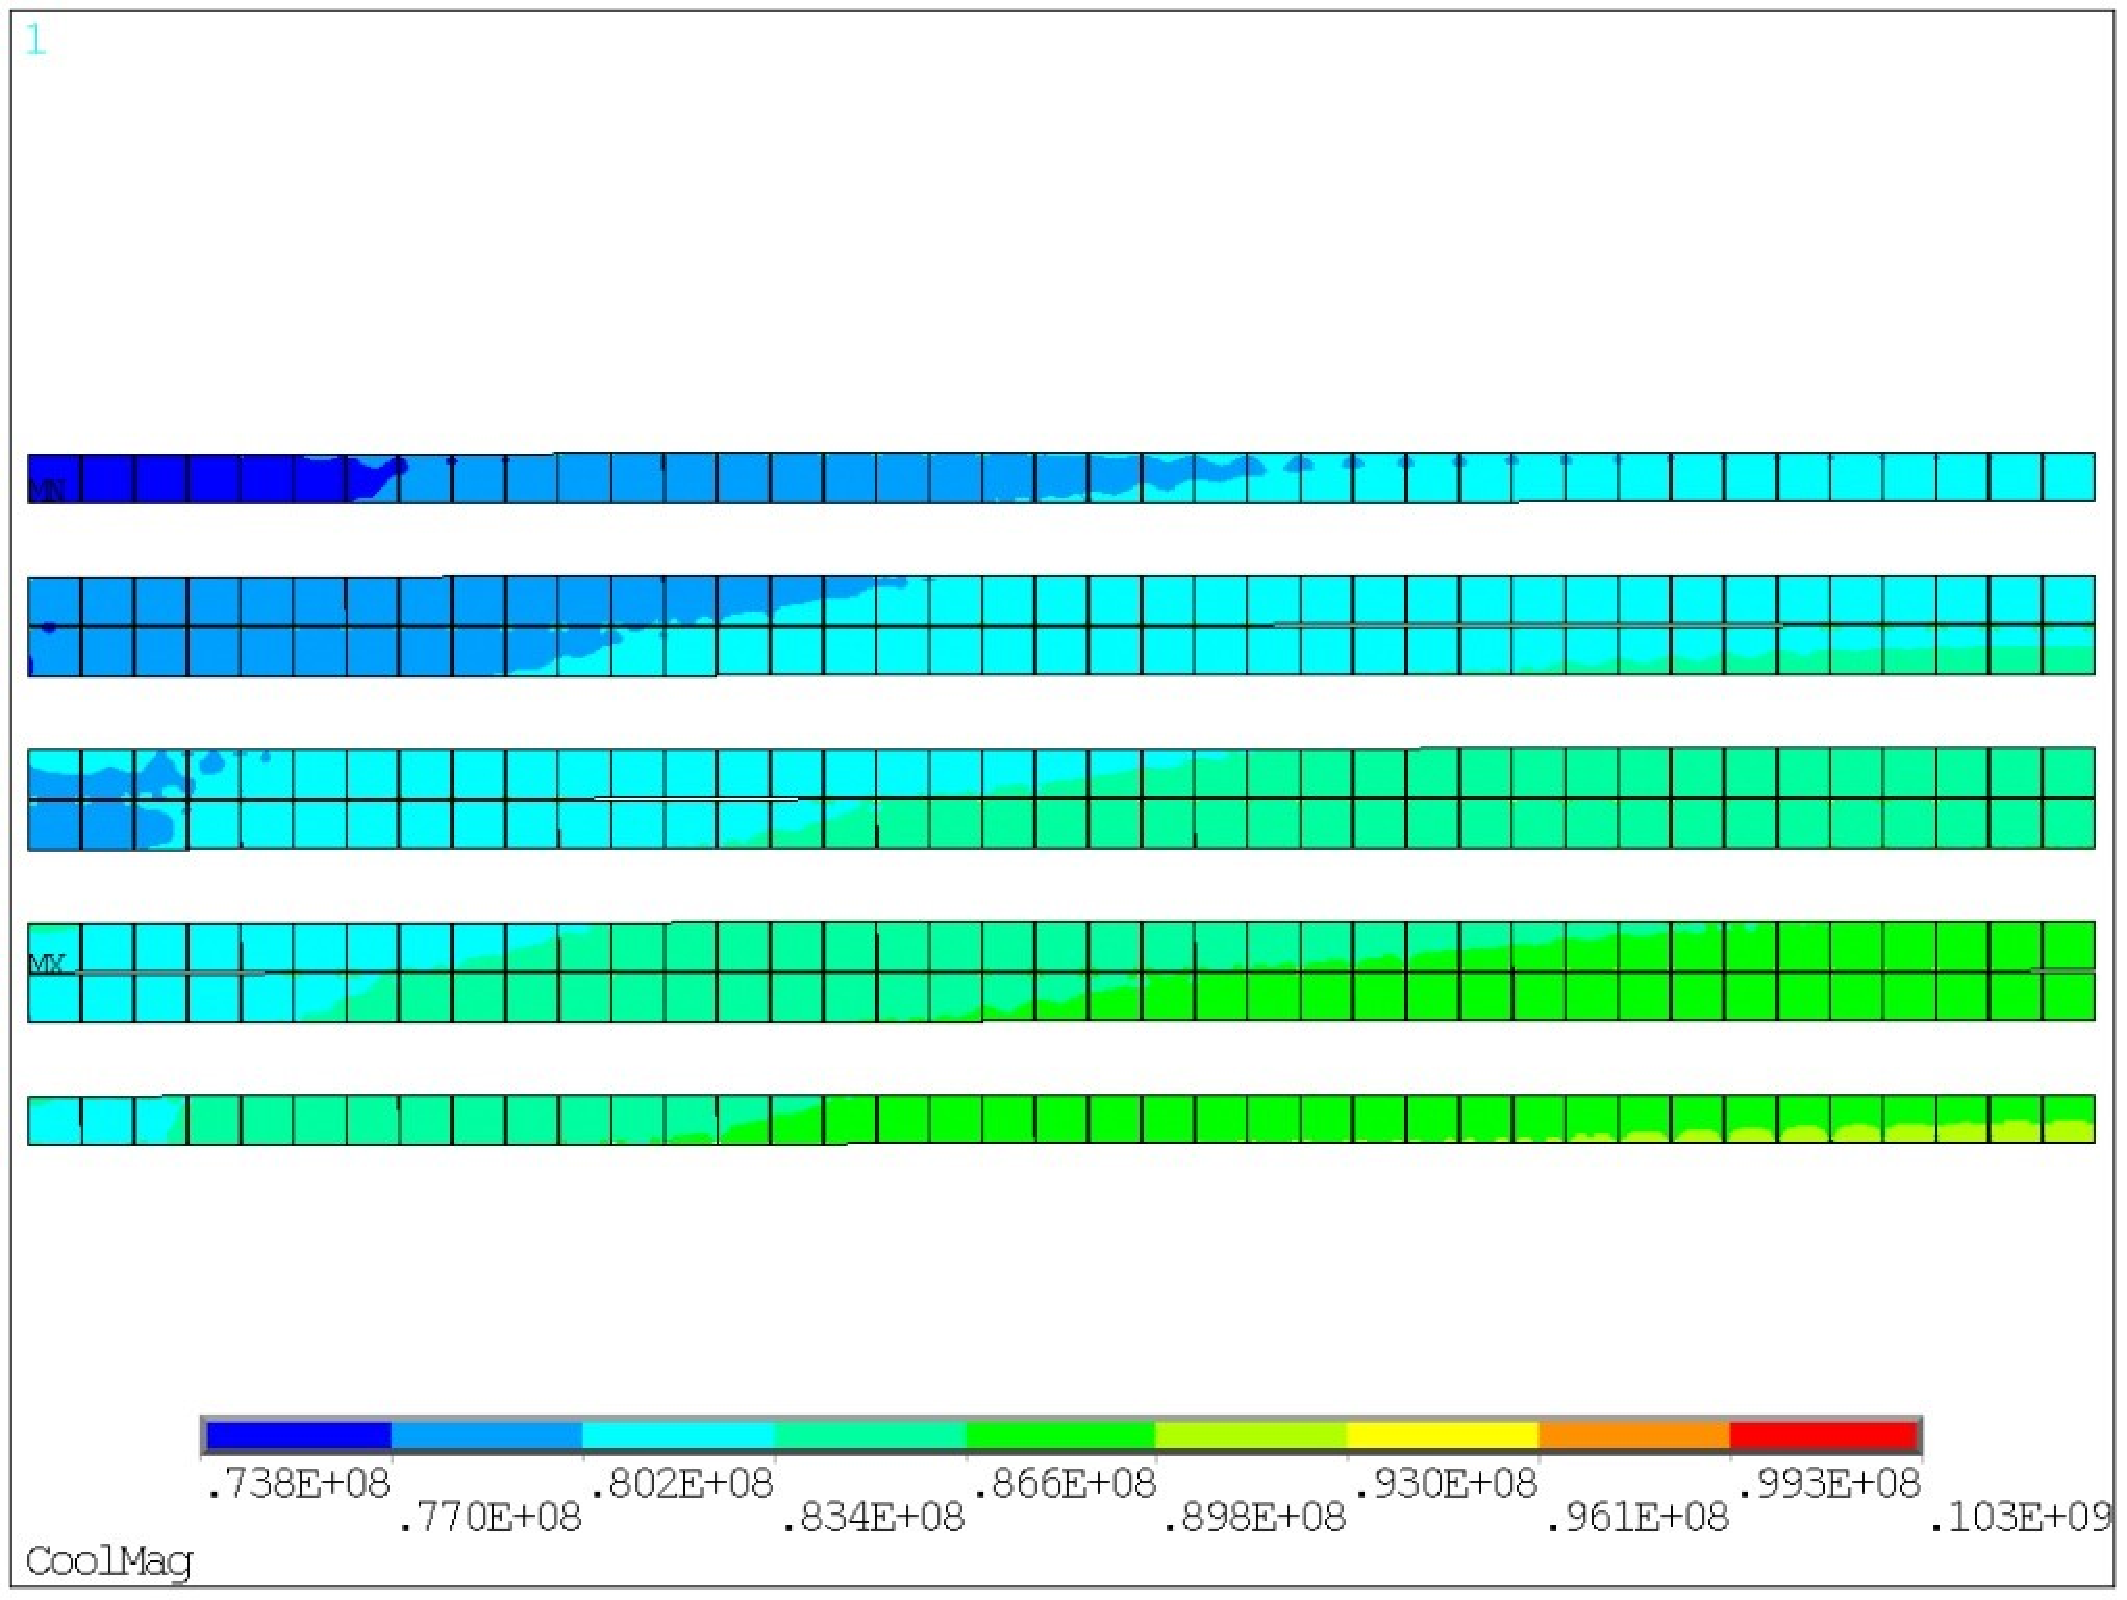
\includegraphics[scale=0.36]{Figures/Magnet/218}
\caption{Coil at 4.2 K, energized, Von Mises distribution of the central coil aluminum alloy}
\label{fig:218}
\end{figure}
\subsection{Preliminary quench analysis}


Introduction: CEPC coil quench protection system, as shown in Fig. 6.19, is based on a dump resistor concept. During a fast dump the power dissipated in it, effectively contributes to driving the whole winding to a normal state. The quench calculation is based on Finite Volume Method (FVM). Use Matlab to simulate the quench propagation in the coils��analyses the hot point temperature and the terminal voltage with time��In the analysis��the coils are just divided into four layers. The inductance is 10.4 H. The operating current is 15779A. The insulation between layers is 1 mm thickness, and between turns is 0.5 mm thickness.


Two different scenarios have been considered: normal external fast dumping and failure of the protection system. The quench starts at the end of first layer, given the temperature of 9 K. Three conditions of dump resistor��1, the protection system failure, Rp=0; 2, Rp=0.05��; 3, Rp=0.1��.
%
\begin{figure}[h!]
\centering
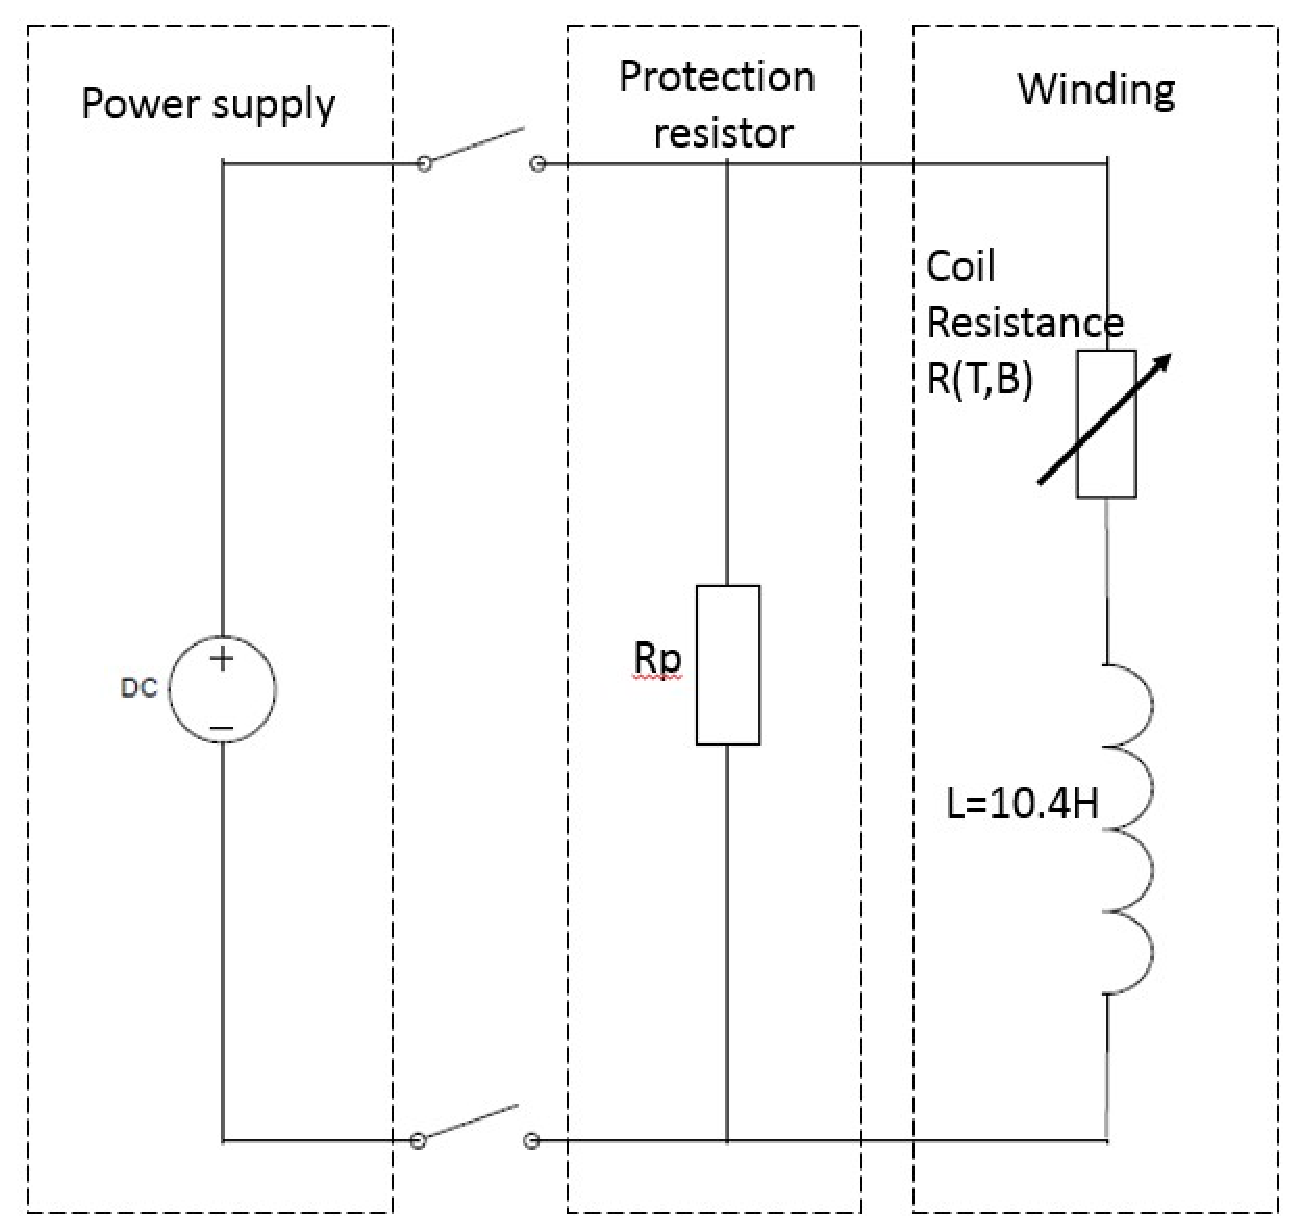
\includegraphics[scale=0.36]{Figures/Magnet/219}
\caption{Equivalent electrical circuit of the quench protection of CEPC}
\label{fig:219}
\end{figure}


Calculation process��All the materials we used are: G-10 CR��Fiberglass Epoxy��, 1100 pure aluminum��6061-T6 aluminum alloy��OFHC Copper RRR=100, NbTi. The curves of the magnet parameters under these three conditions are given in the figures below. Current, resistance, hot temperature and voltage of the magnet are shown. Table 6.8 give the summary of the quench calculation.
%
\begin{figure}[h!]
\centering
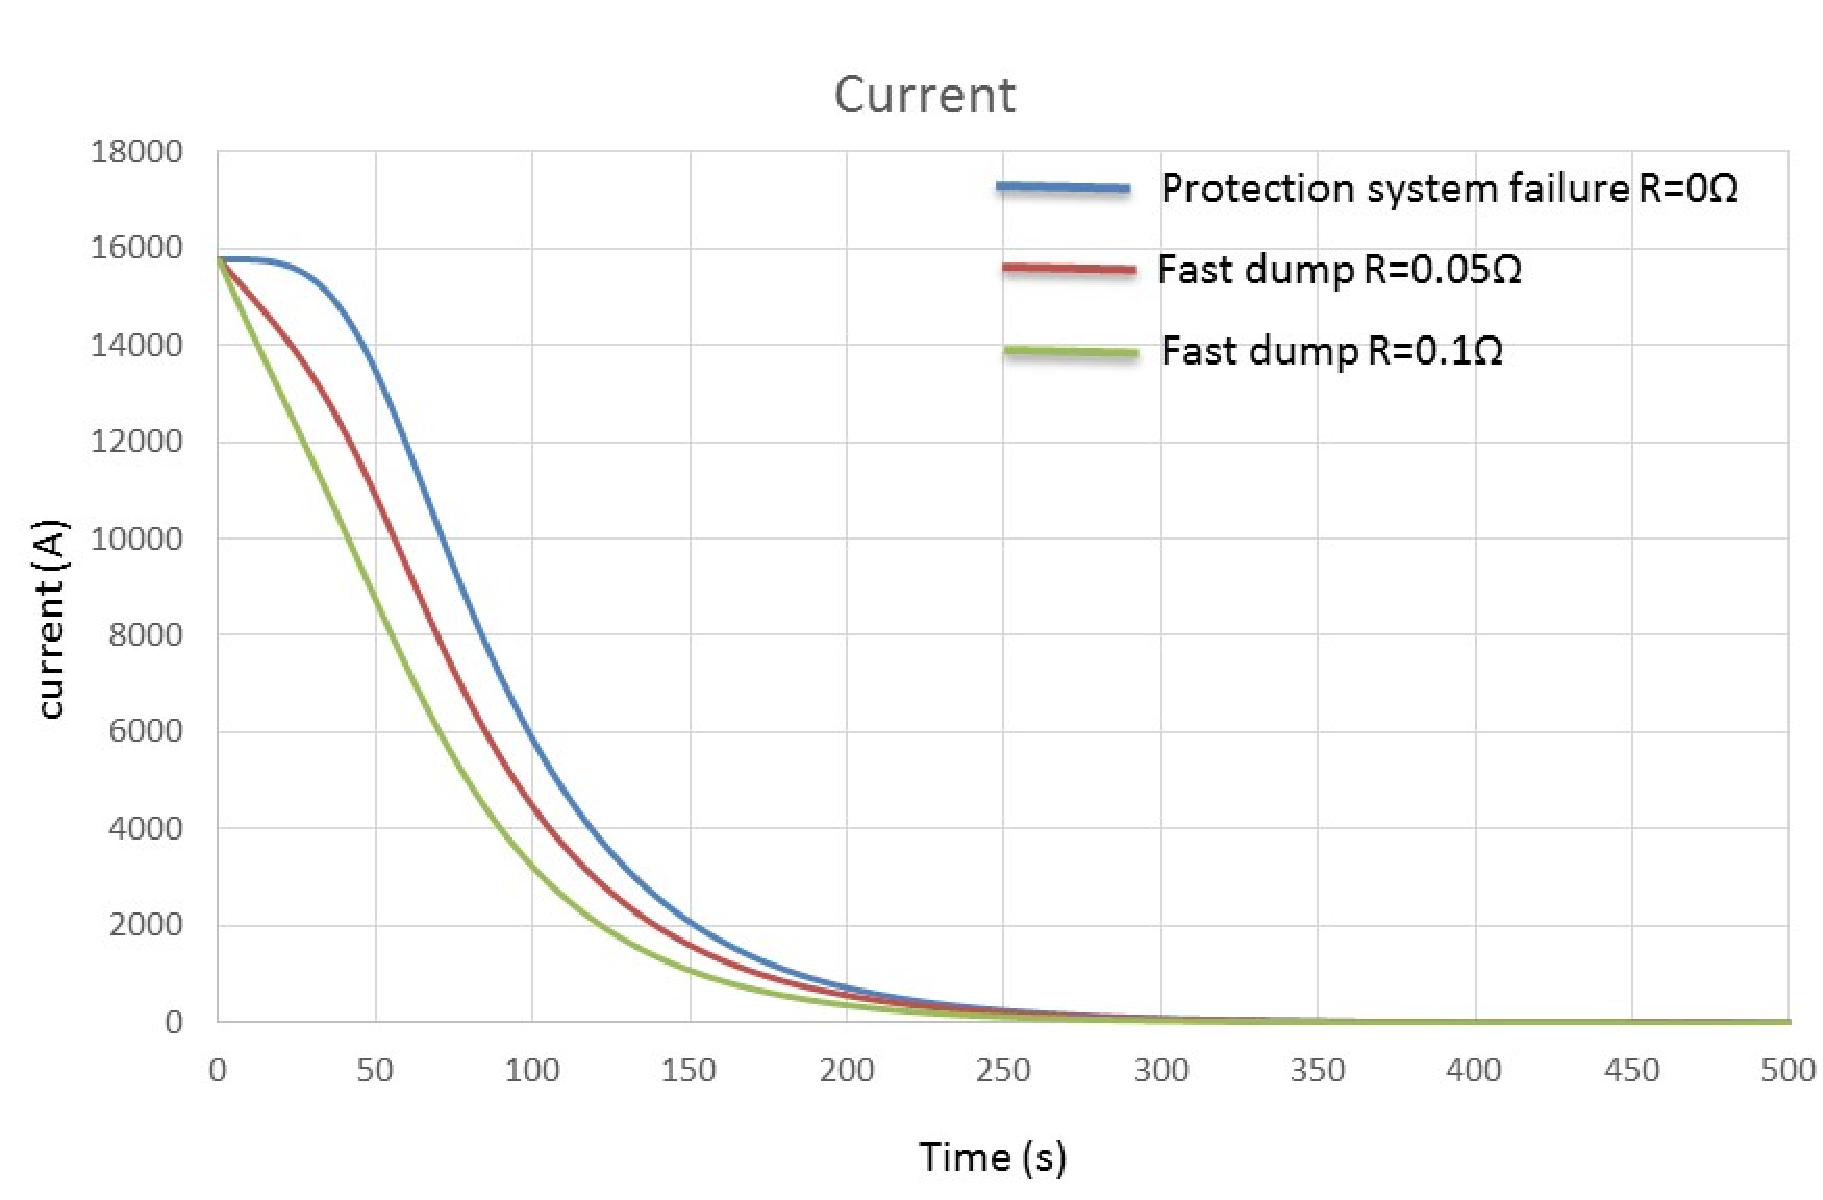
\includegraphics[scale=0.36]{Figures/Magnet/220}
\caption{Comparison of the current profile with protection system failure and with different fast dump resistors}
\label{fig:220}
\end{figure}
%
\begin{figure}[h!]
\centering
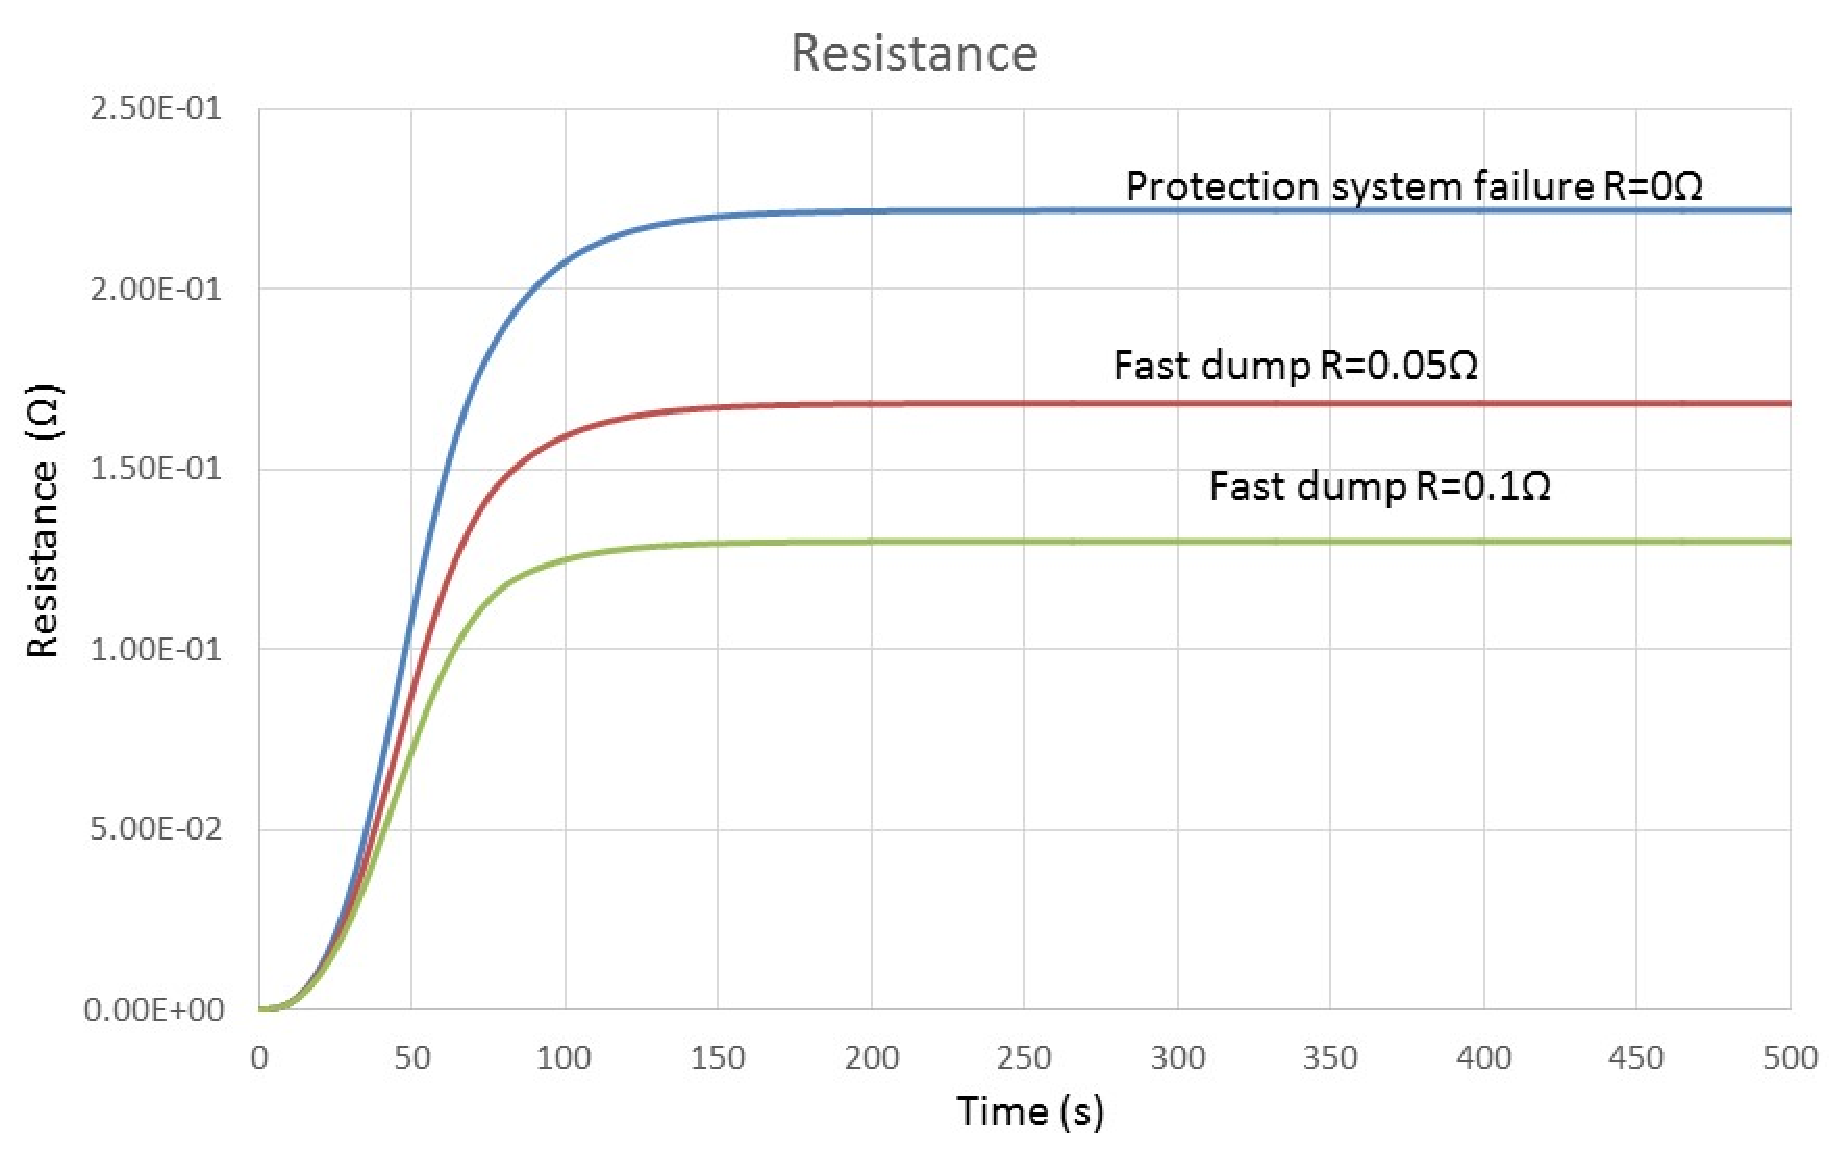
\includegraphics[scale=0.36]{Figures/Magnet/221}
\caption{Comparison of the coil resistance profile with protection system failure and with different fast dump resistors}
\label{fig:221}
\end{figure}
%
\begin{figure}[h!]
\centering
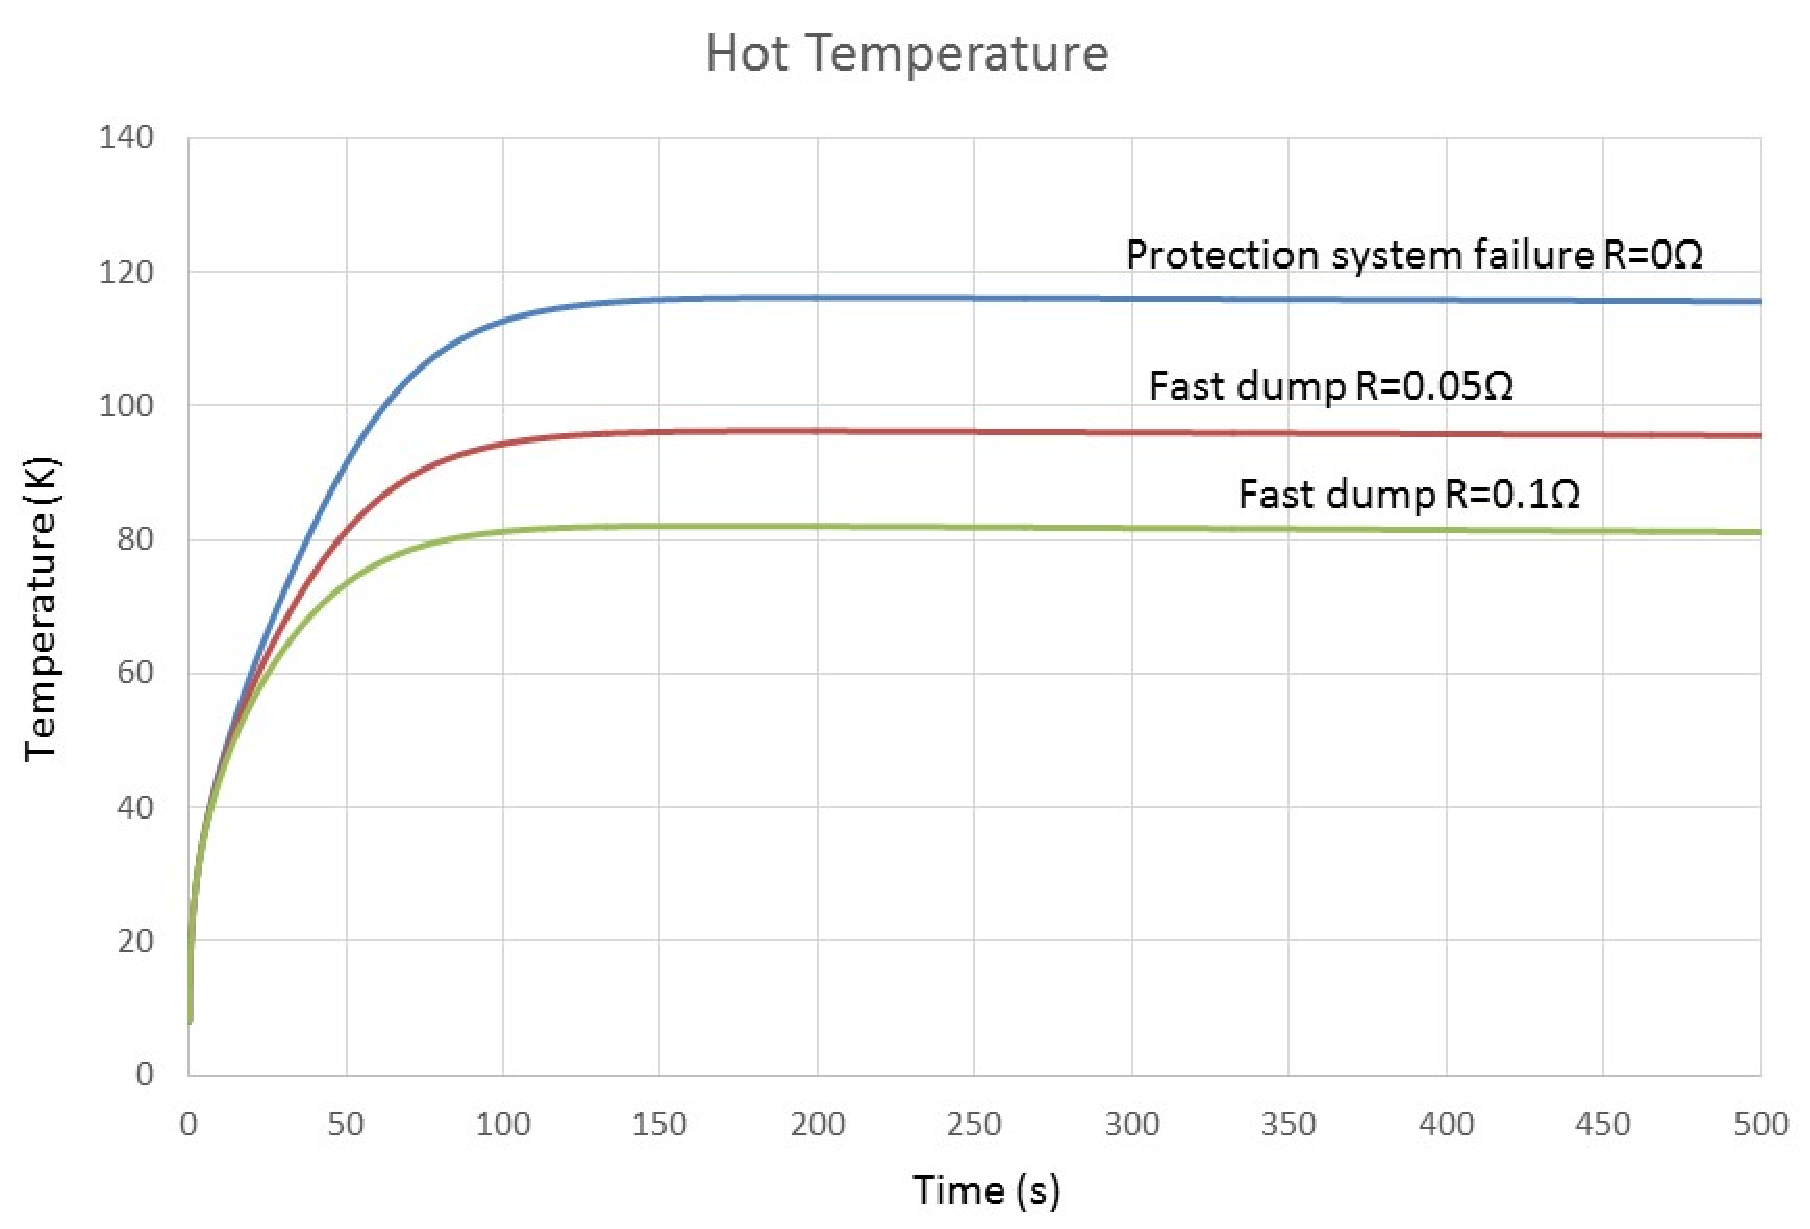
\includegraphics[scale=0.36]{Figures/Magnet/222}
\caption{Comparison of temperature profile with protection system failure and with different fast dump resistors}
\label{fig:222}
\end{figure}
%
\begin{figure}[h!]
\centering
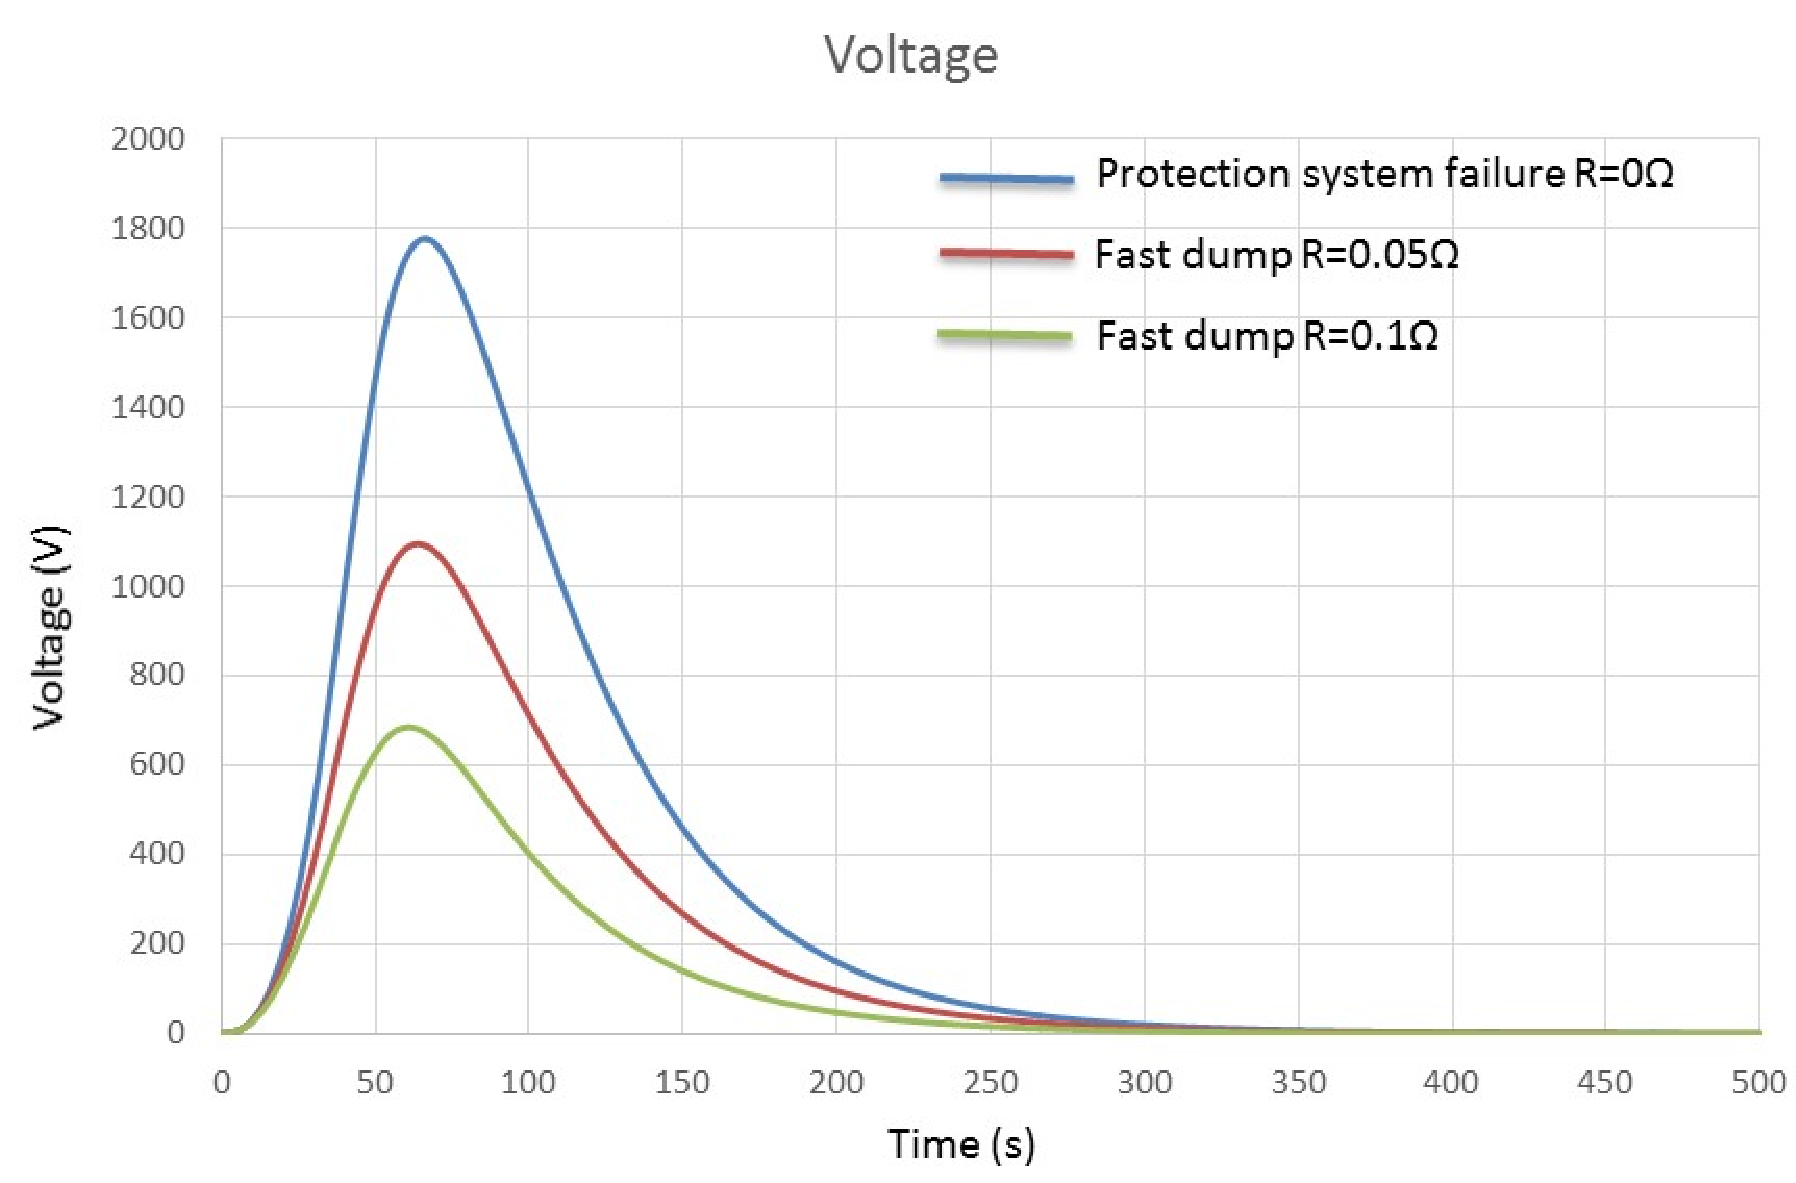
\includegraphics[scale=0.36]{Figures/Magnet/223}
\caption{Comparison of the coil voltage profile with protection system failure and with different fast dump resistors}
\label{fig:223}
\end{figure}
%
\begin{table}[!h]
	\centering
	\begin{tabular}{p{4cm}|p{4cm}|p{4cm}|p{4cm}}
		\hline
		Fast dump resistance Rp & 0 $\Omega$ & 0.05 $\Omega$ & 0.1 $\Omega$ \\
		\hline
		Average final coil temperature & 136 K & 113K & 96K \\
		\hline
		Effective time constant(the current is I=I0/e=6833A) & 90s & 80s & 68s \\
		\hline
		Magnet final resistance & 0.25 $\Omega$ & 0.19 $\Omega$ & 0.15 $\Omega$ \\
		\hline
        Max voltage & 2323 V & 1478 V & 946 V \\
		\hline
        Extracted energy & 0 & 8.27e8 J & 1.279e9 J \\
		\hline
        Extracted energy ratio & 0 & 46\% & 71\% \\
		\hline
	\end{tabular}
	\caption{ Influence of Rp on quench characteristics}
	\label{tab:structure}
\end{table}
\section{HTS/LTS Superconductor Options}
\subsection{HTS plan background}


The center magnetic field strength of CEPC detector magnet is 3 T; the length of the magnet is about 15 meters; inner diameter is 7 m. If we use LTS (low temperature superconducting) plan, it is easier and more mature, but high temperature superconductor is the trend of the superconducting development, especially in the high strength field (greater than 16 T) detector magnets and accelerator magnets, it is only the HTS can be achieved, so we need to accelerate the research of high temperature superconducting applications, accumulate high temperature superconducting magnet processing experience, grasp the magnet processing technology. Compared with the use of low temperature superconducting, the high temperature superconducting detector has the following advantages: 1. maybe the cost of the magnet will be reduced; 2. the security residual is large, the magnet is stable and not easy to quench; 3. HTS is not affected by irradiation; 4. Less material of HTS; 5. Coil winding is relatively easy. The coil can be made into a single pancake or double pancake, and then spliced; 6. Working at a relatively high temperature (20 K), the cooling structure is easy to do; 7. Use YBCO in bulk to reduce YBCO cost and promote the development of high temperature superconducting technology and related enterprises; 8. Lay the foundation for future high field magnets.


The second generation of practical HTS conductors, chemical formula YBa2Cu3O7 (YBCO). It is mainly produced by coating method (CCC - coated conductor composite): using chemical deposition or physical coating methods coating a layer of YBCO superconducting film on the alloy substrate. The cost of this kind of conductor is low. Figure 1 shows the structure diagram of YBCO (from Shanghai superconductor Company)
\begin{figure}[h!]
\centering
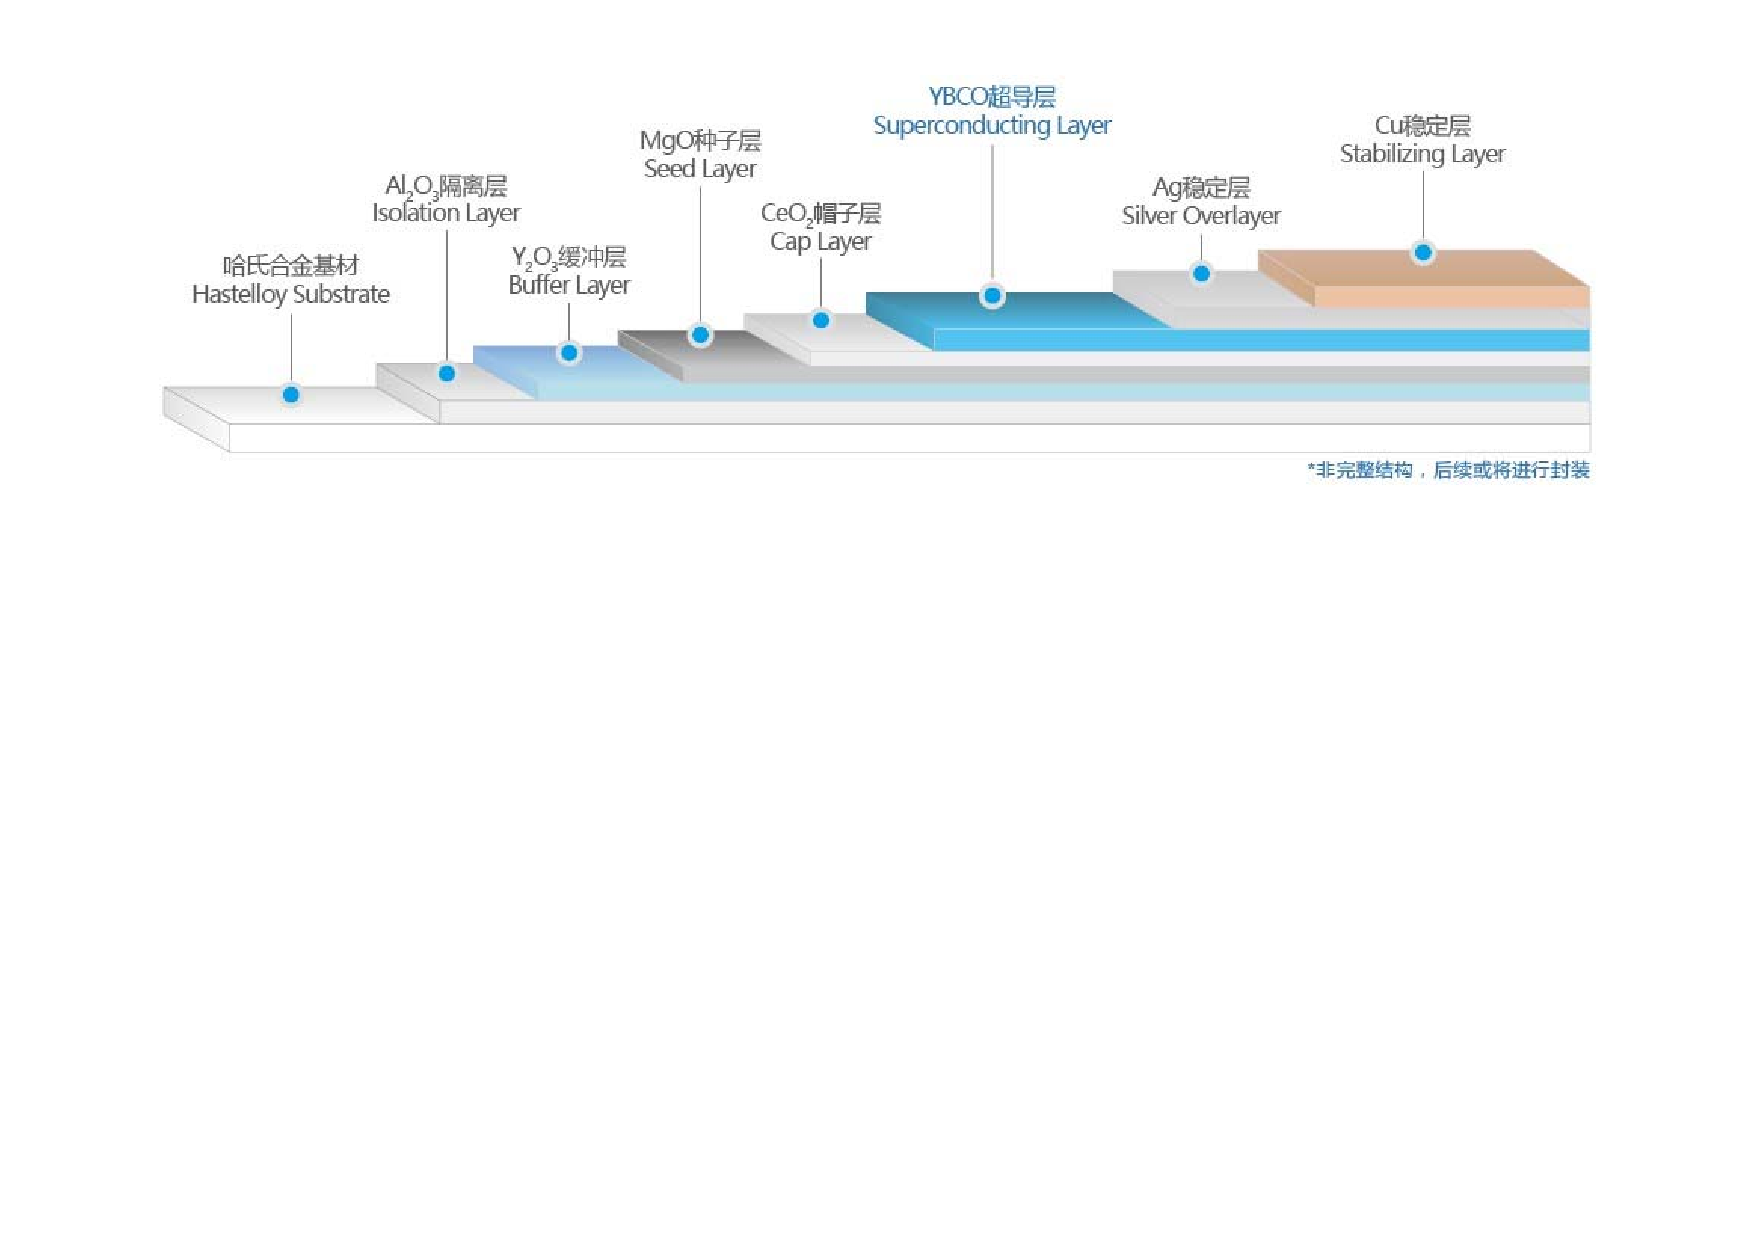
\includegraphics[scale=0.36]{Figures/Magnet/31}
\caption{The structure diagram of YBCO}
\label{fig:31}
\end{figure}


The high temperature superconducting YBCO has a huge advantage in the high field. The relationship between the critical current and magnetic field of various superconducting materials can be seen from figure 2. The advantage of HTS is very obvious when the magnetic field is greater than 20 T. When it is greater than 25 T, we can only use YBCO and 2212 HTS wires. The CEPC detector magnet is also an application of HTS. Because the field is not high, the working temperature can be increased to 20K or even higher, then the requirements for the refrigeration system can be reduced.
\begin{figure}[h!]
\centering
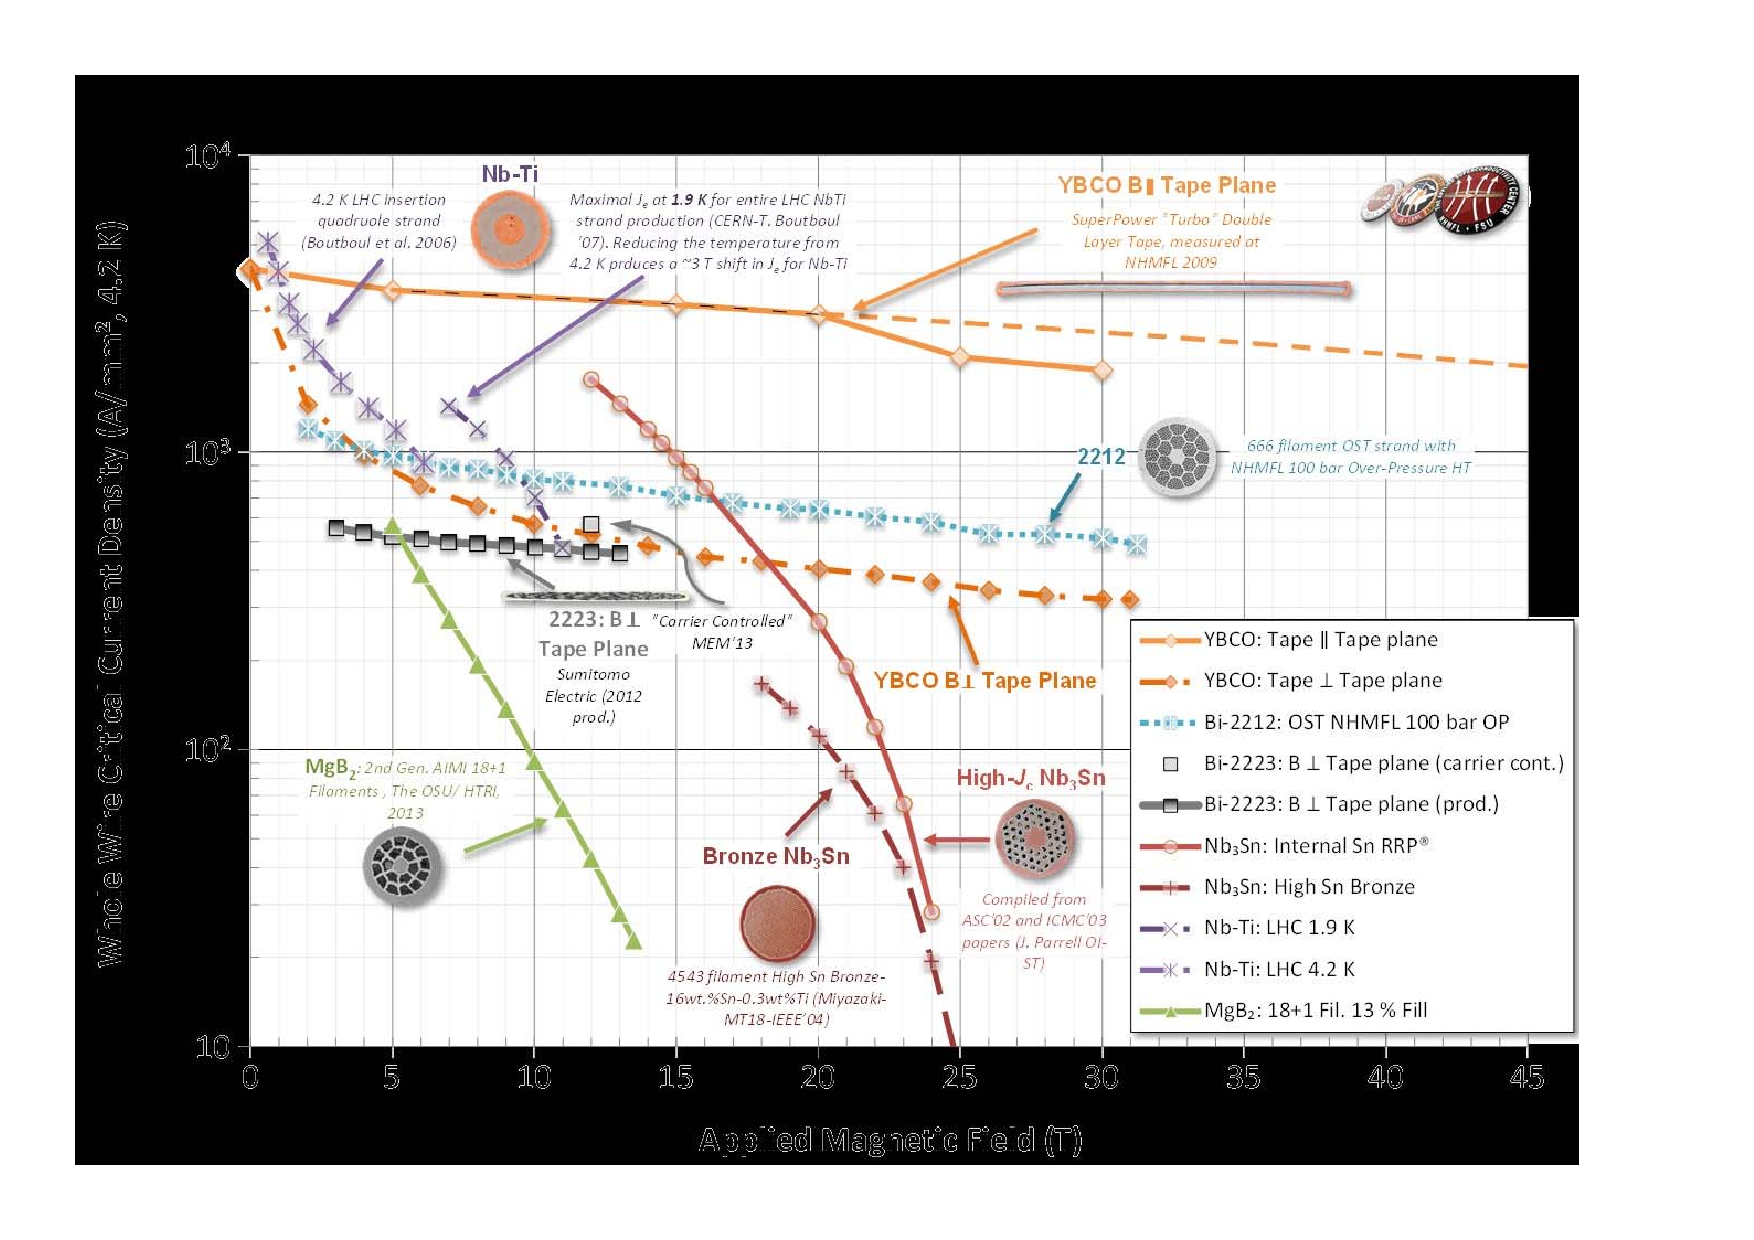
\includegraphics[scale=0.36]{Figures/Magnet/32}
\caption{The relationship between critical current and applied magnetic field of different superconducting materials}
\label{fig:32}
\end{figure} 
\subsection{The latest development of high temperature superconducting cable}


Why do we need to study high temperature superconducting cable? What are the advantages of high temperature superconducting cable? Large detector magnet or accelerator magnets and other magnets generally use cable to wind, its advantages are: 1, increase the reliability of the coil, when one wire or a few wires of the cable quench, other wires can also shunt the current of the cable. Then the magnet would not quench due to a small disturbance; 2. The cable has a lower demand for power supply, and the inductance of single superconducting wire is very large, so we need a higher voltage of the power supply, and the cost of large power supply is very high; 3. Less demand of HTS wire. If the cable is used, the single length of the superconducting wire can be reduced to the order of 100 meters, which can greatly reduce the cost of the superconducting wire.


Some institutes have been developing high-temperature superconducting cables, and so far there has not been a mature, mass-used two-generation high temperature superconducting YBCO cable. Different institutes have different schemes, each has its own advantages and disadvantages, suitable for different types of magnets. Figure 3 shows different YBCO cables, TSTC (Twisted Stacked-Tape Cable) by MIT, CORC (Conductor on Round Core) by ACT (Advanced Conductor Technologies LLC) and RACC (Roebel Assembled Coated Conductor) by General Cable Superconductors Ltd. These cables are also in the lab phase, not in batch applications. For large detector magnets, suitable cables need to be studied.
\begin{figure}[h!]
\centering
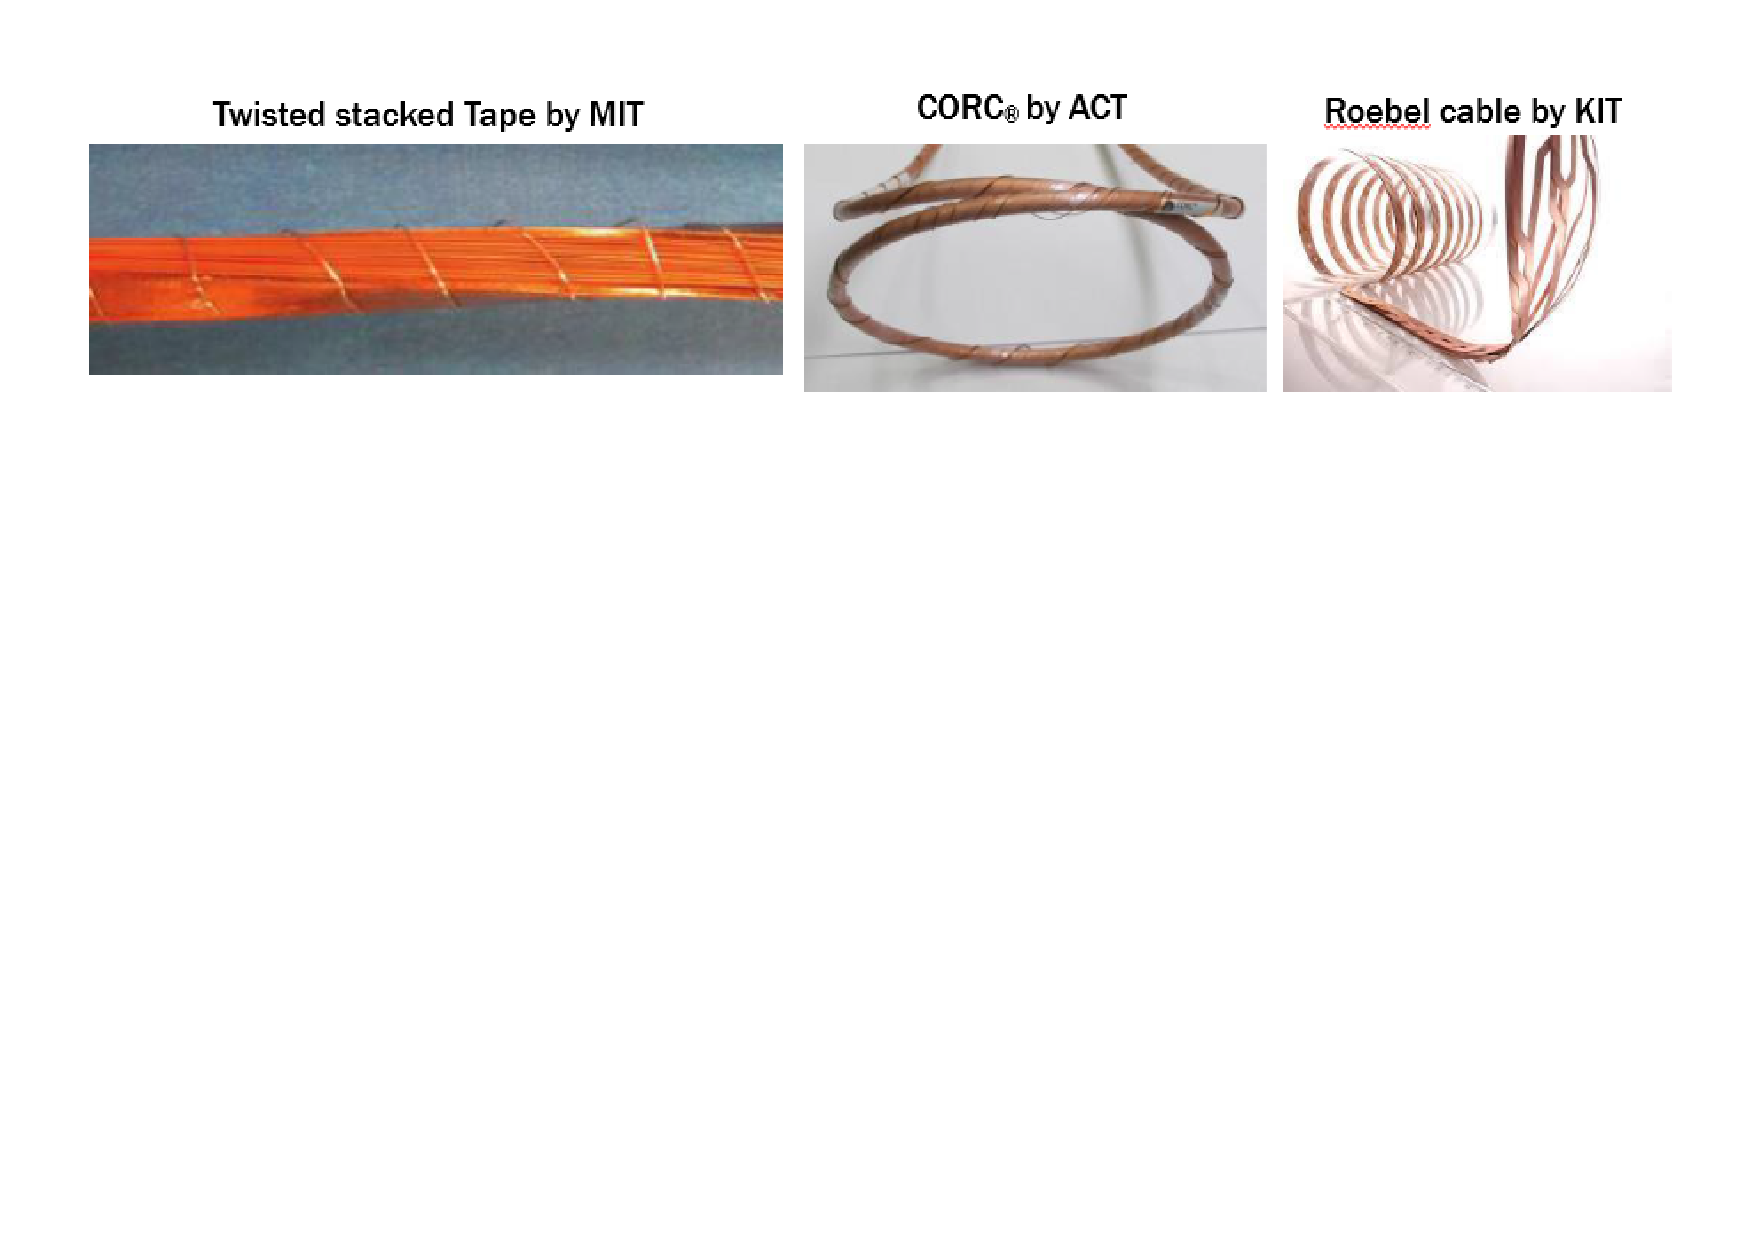
\includegraphics[scale=0.36]{Figures/Magnet/33}
\caption{different YBCO cables}
\label{fig:33}
\end{figure}


  
The advantages of TSTC are simple, high engineering current density, high length ratio of cable to tape length and isotropic J(B). The disadvantage is that it is suitable for winding compact small size magnets. The advantages of CORC cable is the round cable that can be bend freely and isotropic J(B). The disadvantages are low cable conductor length ratio and relatively lower engineering current density. The advantages of Roebel cable are flat cable and high engineering current density. The disadvantages are conductor waste and anisotropic J(B). It is also suitable to wind large detector magnet.
  

The requirement of detector magnets is long time stable. In this way we can develop a new kind of cable based on HTS strips, welding the HTS strip with solder to form a kind of stack form. For example, we use YBCO strip with 12mm width and 0.5mm thick to weld ten layers together to form a 12mm wide and 5mm thick YBCO cable. If each trip can carry 800 A current, then 10 layers cable can carry 8000 A current. The disadvantage of this cable is that when excitation or demagnetization, this cable has a strong coupling effect, if the current changes too fast, it can affect excitation or demagnetization. We can use slow excitation or demagnetization to avoid strong electromagnetic coupling. Figure 4 shows the YBCO stack cable diagram. This kind of cable is easy to produce. We also need to study the stack cable, if it is suitable to wind the large detector magnet.
\begin{figure}[h!]
\centering
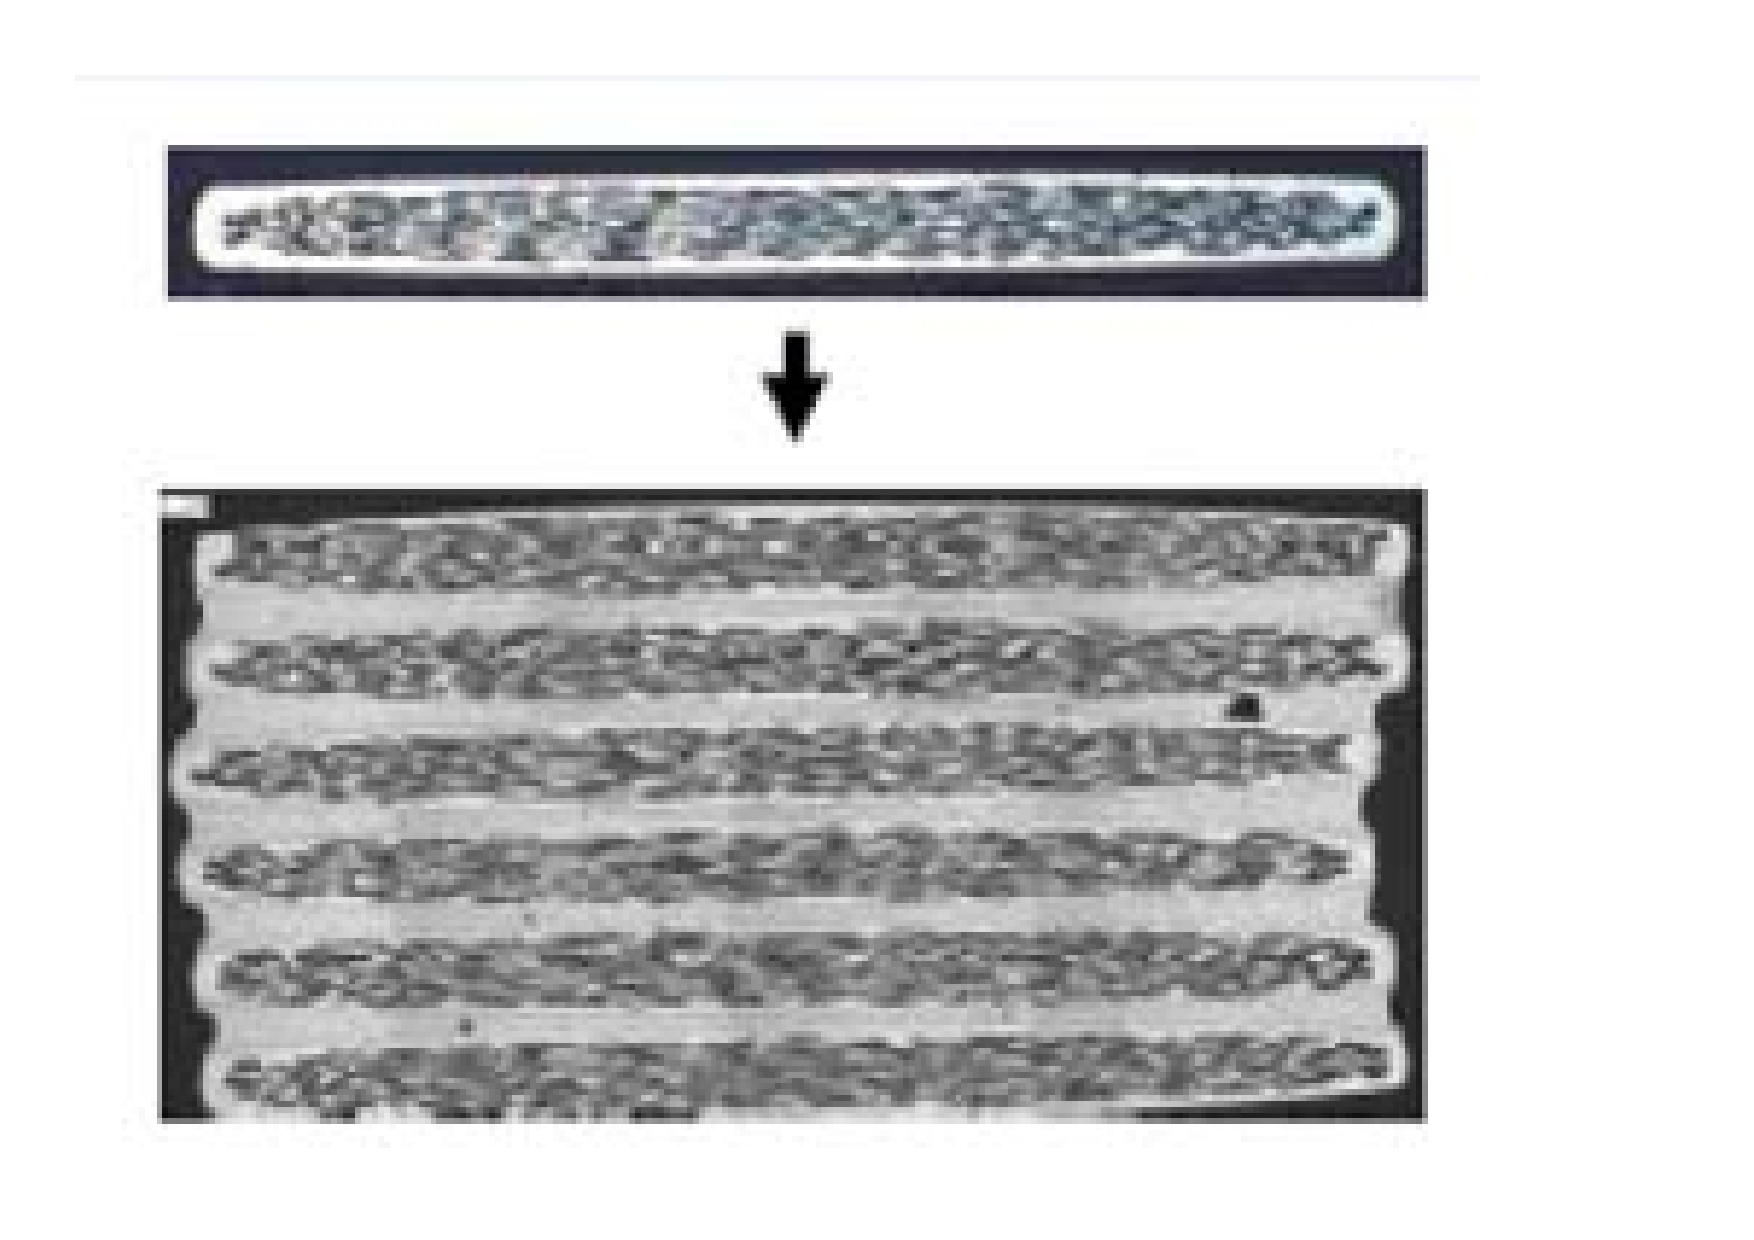
\includegraphics[scale=0.36]{Figures/Magnet/34}
\caption{HTS stack cable}
\label{fig:34}
\end{figure}


As for the selection of HTS cables, we need do further research on which type of cable is suitable for our large detector magnets. The following calculation is based on the simplest stack cable.

\subsection{HTS magnetic design}


The YBCO strip selection, for example Table 1 gives the parameters of Shanghai superconductor Co. We use 12 mm width YBCO strip. Figure 5 is the critical current of the strip at different temperatures and magnetic fields. Table 2 is the critical current at different fields. We select the working current 800 A for each strip and 8000 A for each cable.

%
\begin{table}[!h]
	\centering
	\begin{tabular}{c|c|c|c|c|c|c|c|c}
		\hline
		series & ST-02-E & ST-03-E & ST-04-E & ST-05-L & ST-05-E & ST-06-L & ST-10-E & ST-12-L \\
		\hline
		Post-processing & Copper-plated & Copper-plated & Copper-plated & Laminated & Copper-plated & Laminated & Copper-plated & Laminated \\
		\hline
		Average Ic (77K s.f.) & 45-60A & 75-100A & 80-120A & 45-120A & 120-160A & 120-160A & 200-350A & 200-350A  \\
		\hline
		Wire Width & 2mm & 3/3.3mm & 4mm & 4.8mm & 5mm & 5.8mm & 10mm & 12mm \\
		\hline
        Wire Thickness & 55-95 $\mu$m & 55-95 $\mu$m  & 55-95 $\mu$m & 175-350 $\mu$m & 55-95 $\mu$m & 175-350 $\mu$m & 55-95 $\mu$m & 175-350 $\mu$m \\
        \hline
		Crit.Tensile Stress & >400Mpa & >400Mpa & >400Mpa & >400Mpa & >400Mpa & >400Mpa & >400Mpa & >400Mpa \\
        \hline
		Crit.Tensile Strain & 0.4\% & 0.4\%& 0.4\%& 0.4\%& 0.4\%& 0.4\%& 0.4\%& 0.4\% \\
        \hline
		Current Uniformity & $\pm$5-10\% & $\pm$5-10\% & $\pm$5-10\% & $\pm$5-10\% & $\pm$5-10\% & $\pm$5-10\% & $\pm$5-10\% & $\pm$5-10\% \\
	    \hline
		Min Bending Diameter & 11-15mm & 11-15mm & 11-15mm & 15-20mm & 11-15mm & 15-20mm & 11-15mm & 15-20mm \\
	\end{tabular}
	\caption{ Influence of Rp on quench characteristics}
	\label{tab:structure}
\end{table}

\begin{figure}[h!]
\centering
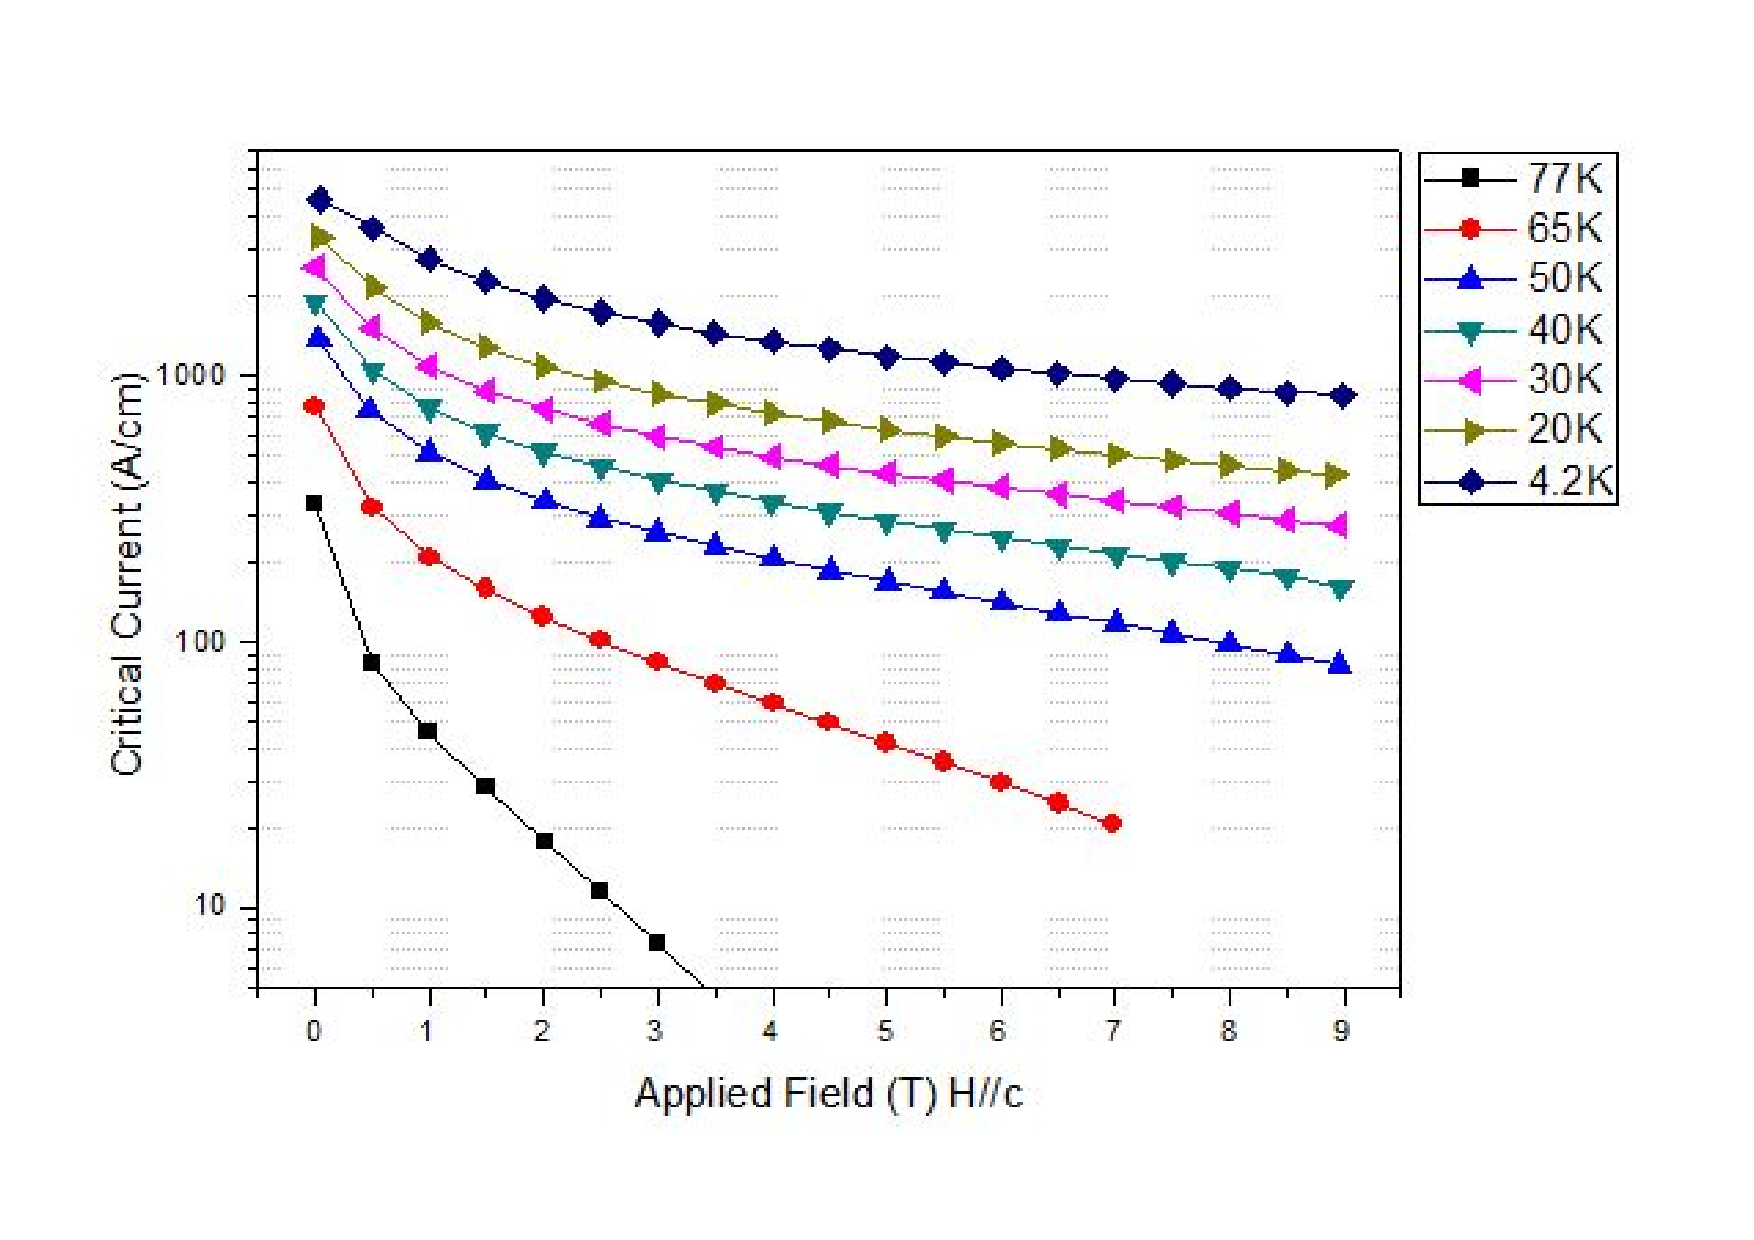
\includegraphics[scale=0.36]{Figures/Magnet/35}
\caption{Critical current at different temperatures and magnetic fields}
\label{fig:35}
\end{figure}

\begin{table}[!h]
	\centering
	\begin{tabular}{c|c}
		\hline
		Magnetic field & Ic (4.2K) \\
		\hline
		2T & 2000A \\
		\hline
		3T & 1700A \\
		\hline
		5T & 1200A \\
		\hline
	\end{tabular}
	\caption{critical current at different magnetic field}
	\label{tab:structure}
\end{table}


The superconducting coils are in the form of multiple double pancakes, with a total of 500 turns and 7.5 meters in length. Radial direction can be divided into five YBCO stack cables, each stack cable contains 10 of 12 mm wide YBCO strips, and the thickness is about 50 mm. Table 3 is the parameters of HTS magnet. Figure 6 shows the magnetic field distribution.


\begin{table}[!h]
	\centering
	\begin{tabular}{c|c|c|c}
		\hline
		Central magnetic field & 3 T & Working current & 7970 A \\
		\hline
		Maximum vertical field on cable & 2.7 T & Ampere-turns & 20000000 \\
		\hline
		Inner diameter of coil & 3.6 m & Inductance & 38.36 H \\
		\hline
		Outer diameter of coil & 3.7 m & Stored energy & 1.2 GJ \\
		\hline
        Length of the coil & 7.5 m & Operating temperature & Less than 20 K \\
		\hline
	\end{tabular}
	\caption{Parameters of CEPC detector magnet}
	\label{tab:structure}
\end{table}

\begin{figure}[h!]
\centering
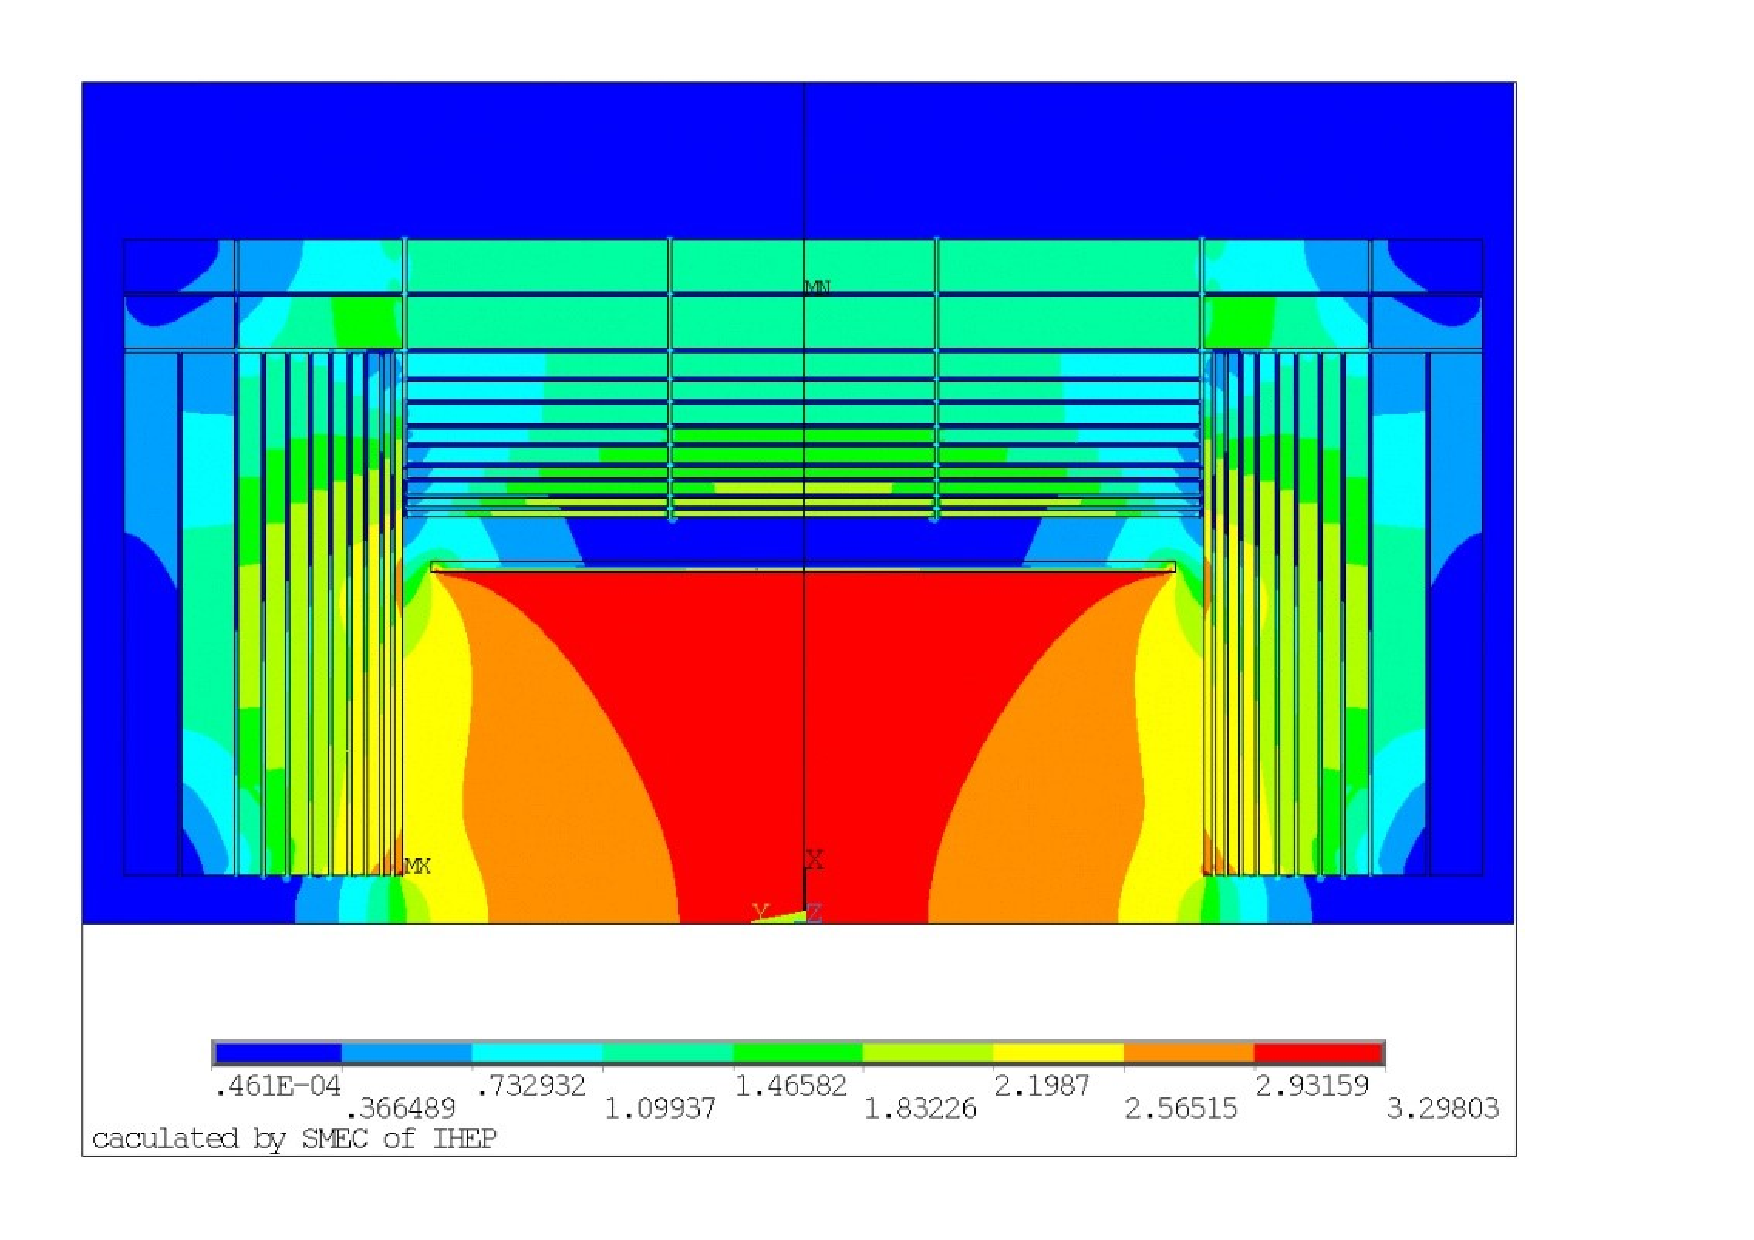
\includegraphics[scale=0.36]{Figures/Magnet/36}
\caption{Magnetic field distribution}
\label{fig:36}
\end{figure}

\begin{figure}[h!]
\centering
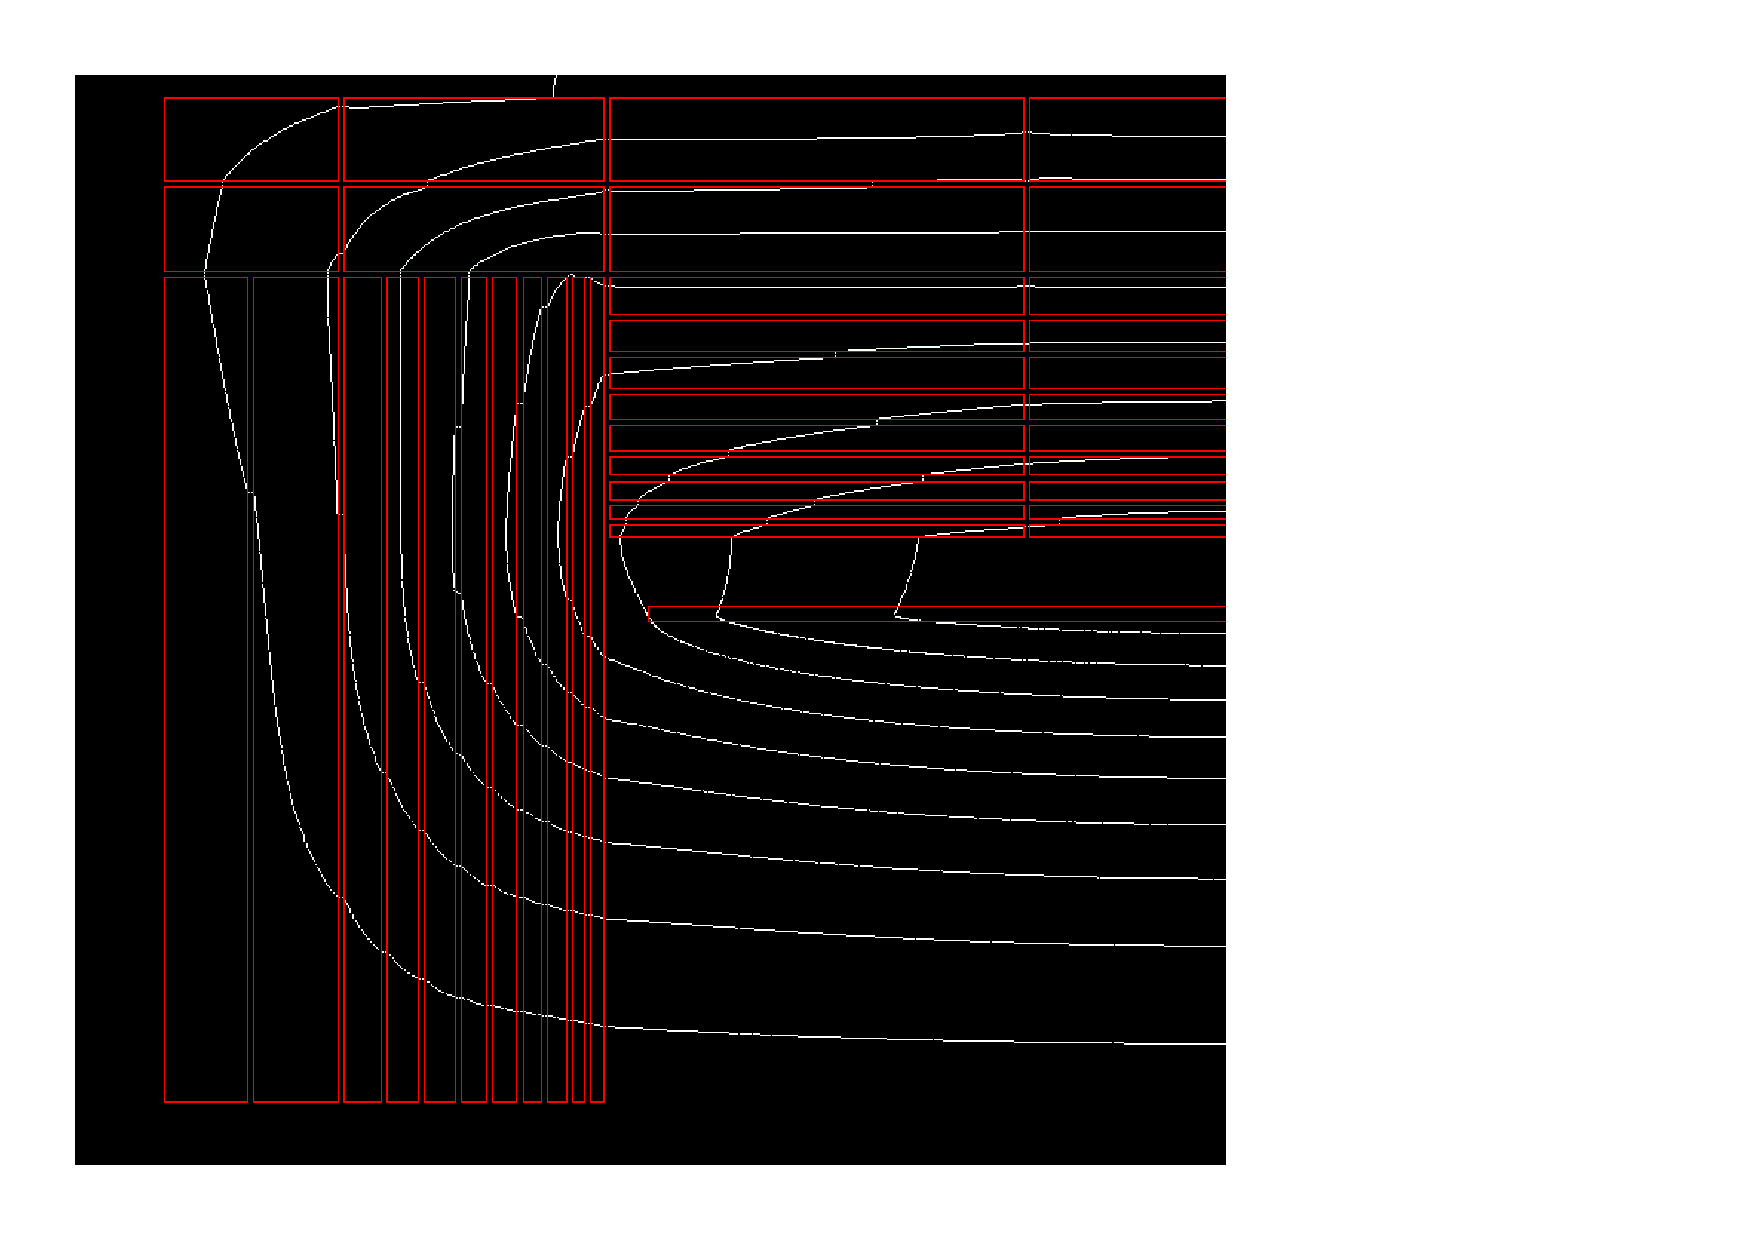
\includegraphics[scale=0.36]{Figures/Magnet/37}
\caption{Magnetic flux distribution}
\label{fig:37}
\end{figure}

Stray field distribution:

\begin{table}[!h]
	\centering
	\begin{tabular}{c|c|c}
		\hline
		 & axial direction & radial direction \\
		\hline
		50Gs & 15m & 13m \\
		\hline
		100Gs & 11m & 9m\\
		\hline
	\end{tabular}
	\caption{stray field region}
	\label{tab:structure}
\end{table}

\begin{figure}[h!]
\centering
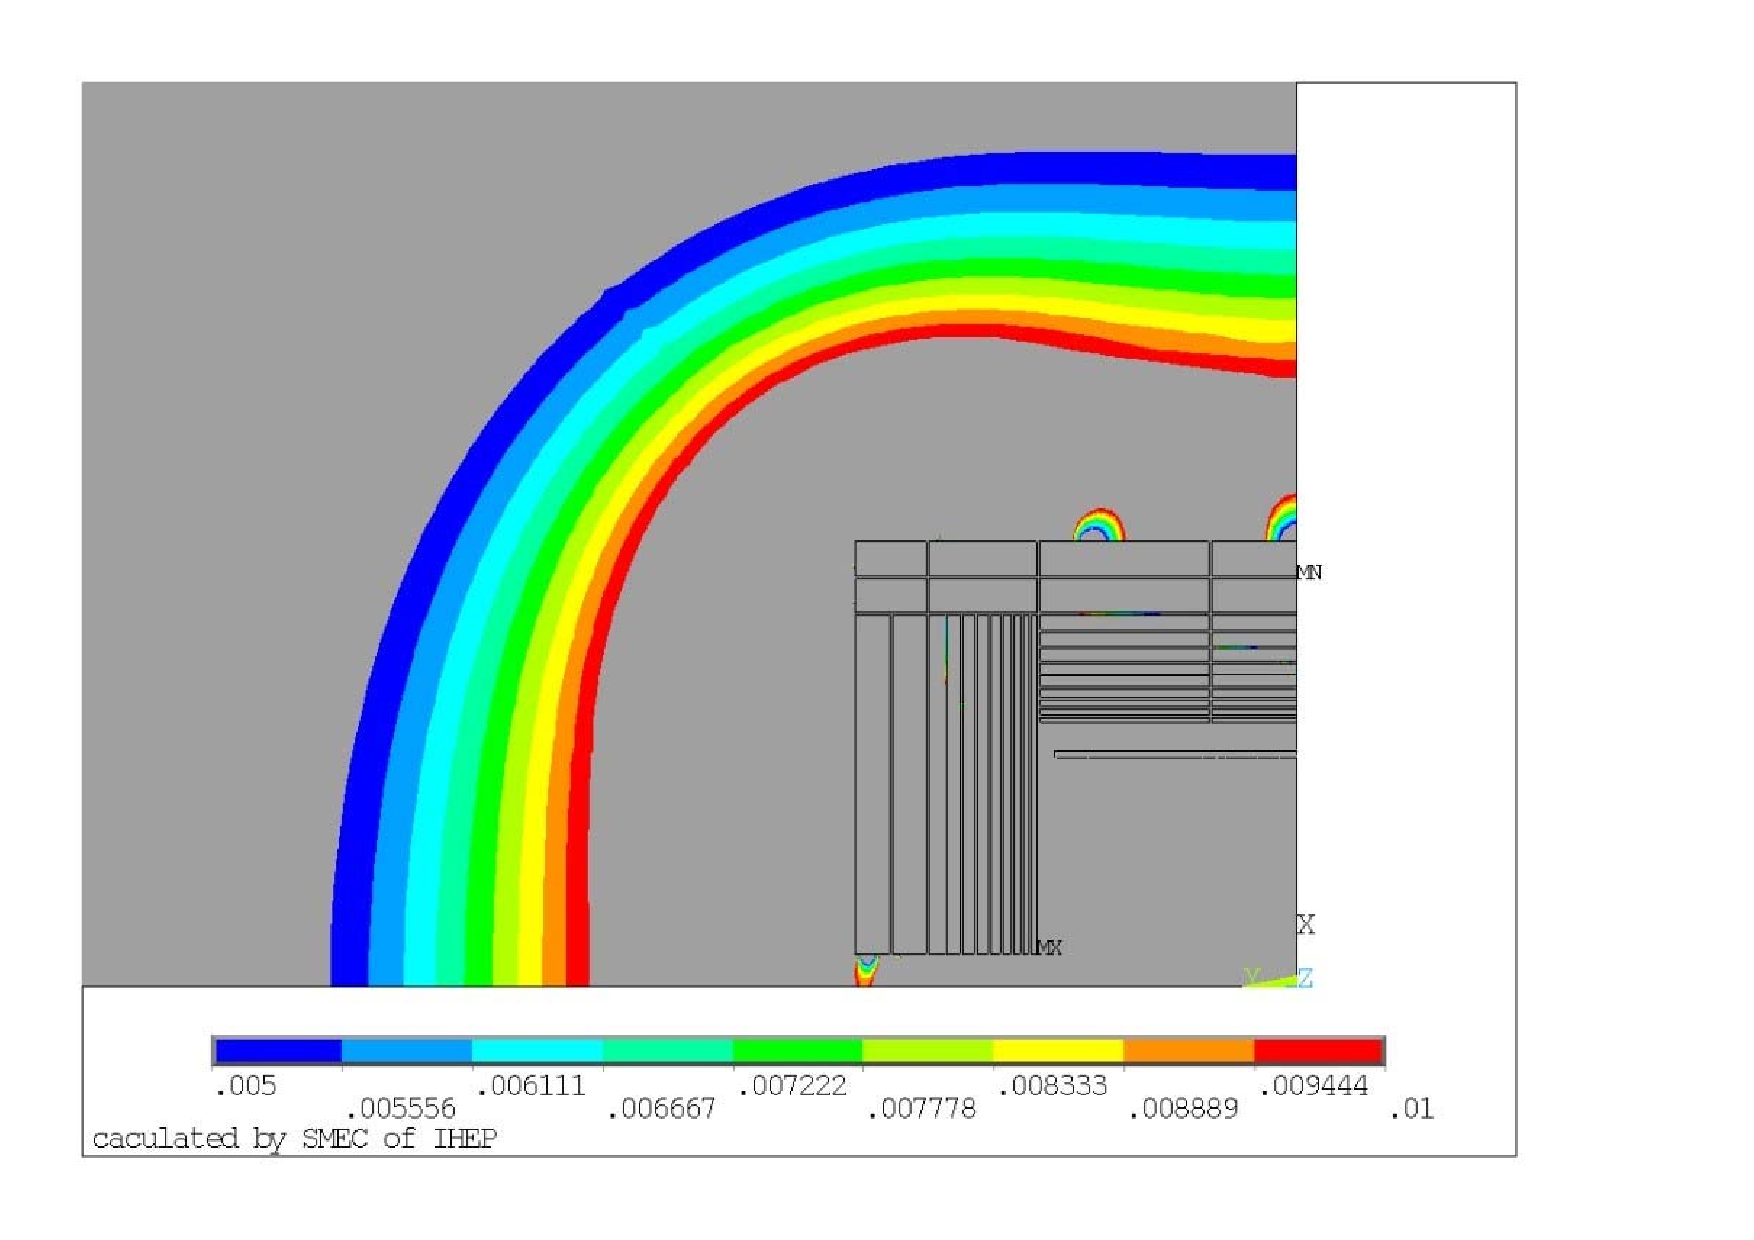
\includegraphics[scale=0.36]{Figures/Magnet/38}
\caption{Stray field distribution of 50 Gs and 100 Gs}
\label{fig:38}
\end{figure}

\subsection{Future work of HTS plan}
I) YBCO cable research. Select proper HTS cable or develop new cable for large detector magnet.
II) Study of HTS coil winding process. How to wind the YBCO coil?
III) Quench analysis. Study the quench detection, transmission and protection of the HTS coil.
IV) Prototype HTS coil development.


\section{Solenoid Coil Design}
\subsection{Solenoid Coil Structure}


The coil has a 4 layer geometry to obtain the 3T center field with a reasonable nominal current, similarly to CMS. The solenoid has 5 modules, which will reduce the degree of difficulty of coil manufacture.
The coil is wound with inner winding technique, where an aluminum alloy support cylinder is used as an external mandrel for the winding. The support cylinder is also used as a mechanical mandrel for the coil and a quench circuit, the cooling tubes welded on the outer radius of the mandrel, where liquid helium circulates, to ensure the temperature of the coil.


A horizontal cryostat was developed for the superconducting magnet, consisting of a vacuum tank and thermal shields (inner and outer) covered with multiple layers insulation (MLI). The stainless steel vacuum vessel is 8.05 m length and 4.25 m outer radius. Two service towers are on top of the vessel to install current leads and phase separator. The vacuum tank, is cantilevered from the central ring of the barrel yoke.
\subsection{R\&D of Superconducting Conductor}


The conductor design is similar to that of CMS. As the forces induced in the conductor by the magnetic and thermal loads are beyond the yield stress of pure aluminium, a mechanical strengthening is envisaged. This consists of a superconducting Rutherford cable, which is sheathed in a stabiliser and mechanically reinforced. Two aluminium alloy profiles are welded by electron beam to the central conductor stabiliser, which is made of high purity aluminium.
The Rutherford cable will be made with NbTi superconducting strands. It is proposed to use cables with similar characteristics to the CMS superconductor, but with a slightly decreased number of strands in the cable.
%
\begin{table}[!h]
	\centering
	\begin{tabular}{c|c}
		\hline
		\multicolumn{2}{|c|}{Superconducting strand in virgin state} \\
		\hline
		Strand diameter & 1.2 mm \\
		\hline
		Cu/NbTi & 1.3 \\
		\hline
        SC strand critical current density & $\ge$ 2700A/mm2 @4.2K,5T \\
		\hline
        Filament diameter & About 55 um \\
		\hline
        RRR of copper matrix & $\ge$ 100 \\
		\hline
        Twist pitch & 1.3 \\
		\hline
        \multicolumn{2}{|c|}{Rutherford cable} \\
		\hline
		Number of strand & 32 \\
		\hline
		Cable transposition pitch & 120mm \\
		\hline
        Compacting ratio & 0.87 \\
		\hline
        \multicolumn{2}{|c|}{Final conductor} \\
		\hline
		Ic degradation during manufacturing & <10\% \\
		\hline
		Nominal design current & 16KA \\
		\hline
        Critical current at 4.2K and 5 Tesla & 50KA \\
		\hline
        Total length of conductor & 31km \\
		\hline
	\end{tabular}
	\caption{ Superconductor characteristics}
	\label{tab:structure}
\end{table}
%


The initial critical current density of strands have a maximum degradation of 5\% ,and the initial RRR of copper matrix of strands have a degradation of 1/3 due to the stranding process, as demonstrated on the tests by IHEP and Toly Co.
The shear strength between copper and pure Al have a minimum value of 30MPa after the inserting process. And other parameters of the superconductor due to the inserting process are on the testing road now.
\begin{figure}[h!]
\centering
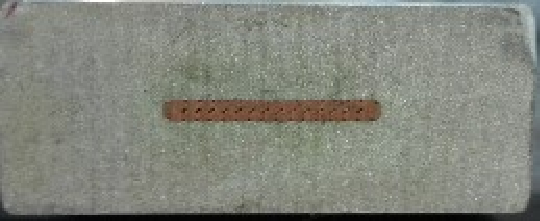
\includegraphics[scale=0.36]{Figures/Magnet/41}
\caption{Samples of shear strength test}
\label{fig:41}
\end{figure}
\begin{figure}[h!]
\centering
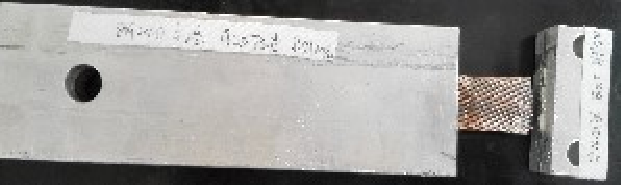
\includegraphics[scale=0.36]{Figures/Magnet/42}
\caption{Samples of shear strength test}
\label{fig:42}
\end{figure}
\begin{figure}[h!]
\centering
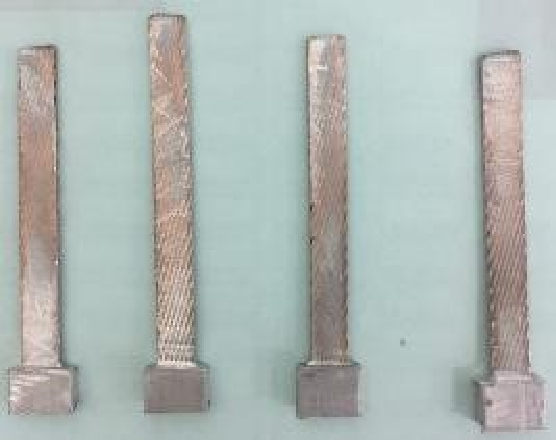
\includegraphics[scale=0.36]{Figures/Magnet/43}
\caption{Samples of shear strength test}
\label{fig:43}
\end{figure}
\subsection{Coil fabrication and assembly}


The coil supporting cylinder consist of five modules, three longer modules in the middle and two shorter ones at the end. All modules are built with aluminium alloy 5083, which inner surfaces are high precision machined and cooling tubes are welded on outer surface. The three longer modules have two flanges and tube joints at each end. The two shorter ones have only one flange at the end and the tube joints at this side too, and the support rods are arranged on the other side.


The coil is wound with the so-called inner winding technique, where the support cylinder is used as an external mandrel for the winding with a vertical axis. The five modules will be wound, immersed and cured individually.


The five coil modules are assembled together by the assembly tooling in the vertical position. They are assembled from one side to the other side. First, one short module is put on the assembly tooling in the vertical position, and then a longer one is put on it, and the flanges of the two modules are connected and the tube joints are welded, thus the two modules are assembled together. According to this method, the other three modules will be assembled together one by one.
\section{Magnet Cryogenics Design}
\subsection{Preliminary Simulation of the Thermosyphon Circuit}
\subsubsection{Computational model and mesh}


CEPC Detector Superconducting Magnet is cooled by the welding U-shaped pipe outside the coil, which using the thermosyphon principle. The thermosyphon circuit consists of three parts: the supplying pipe, the cooling pipe and the returning pipe. The liquid helium absorbs the heat in the cooling pipe and phase change occurs, so the pressure in the cooling pipe changes and a gas-liquid two-phase flow is formed under the pressure difference between the two sides of the circuit. In order to study the phase transition process of helium in the circuit, the original circuit is simplified and the constant mass flow is used instead of the original pressure driving flow. So a single tube model is established (shown in Figure 6.5.1). Figure a show a 10:1 scale model and Figure b show a schematic diagram of 1:1 scale model. The entire circuit uses a uniform diameter of 14mm, the circuit place vertically and direction of gravity is downward vertically.
\begin{figure}[h!]
\centering
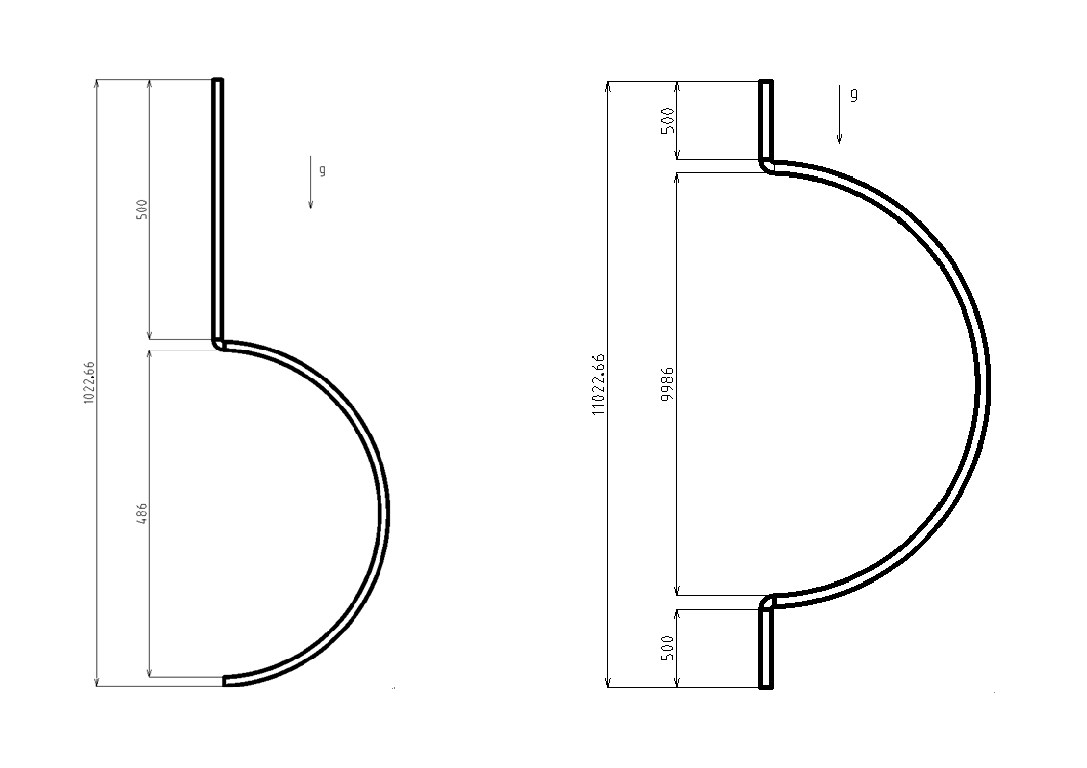
\includegraphics[scale=0.36]{Figures/Magnet/51}
\caption{a. The 10:1 scale model  b. The 1:1 scale model (schematic diagram)  The computational model (mm)}
\label{fig:51}
\end{figure}
\begin{figure}[h!]
\centering
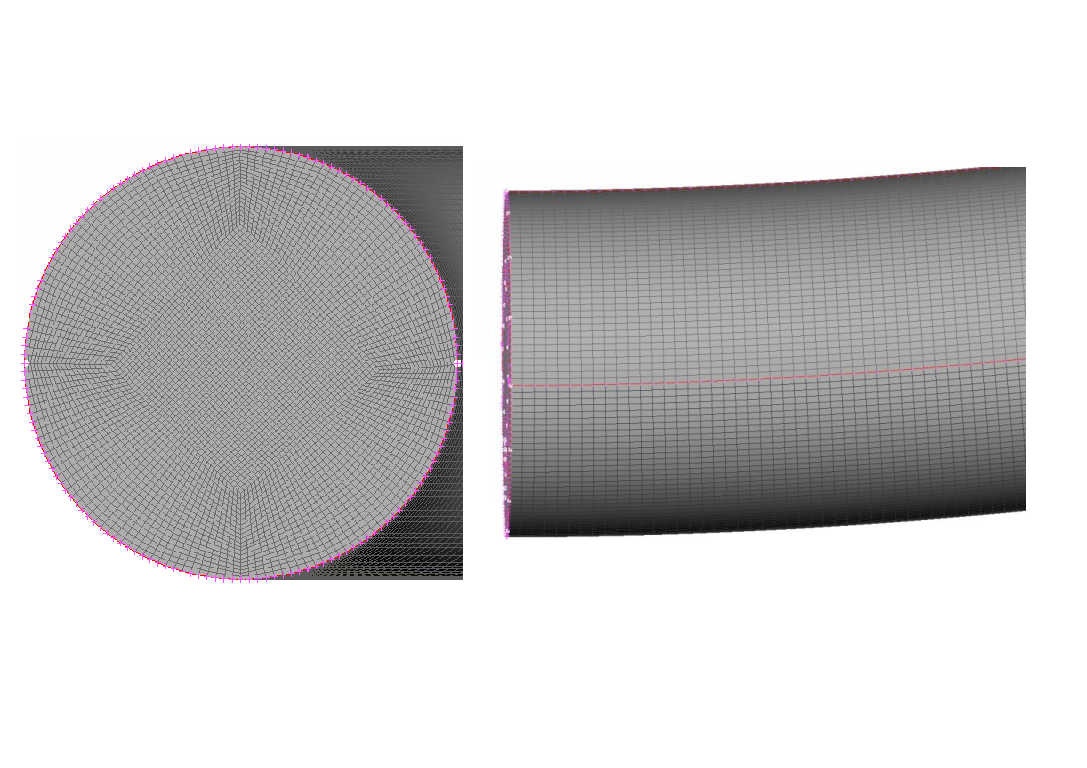
\includegraphics[scale=0.36]{Figures/Magnet/52}
\caption{a. Cross-section mesh    b. Lateral mesh   The mesh shape}
\label{fig:52}
\end{figure}


ANSA is used to generate the mesh of the above three-dimensional model with a total number of 9.84 million for 10:1 scale model and 3.74 million for 1:1 scale model (still in the test stage), the mesh shape is shown in Figure 6.5.2. Because the scale of the latter is bigger than the former, the mesh setting of the 10:1 scale model is not applicable to 1:1 scale model and the simple simulation of 10:1 scale model was started early. In order to capture the accurate phase transition process and obtain accurate simulation results, a smaller mesh and time step is needed. Meanwhile, the density increase for the mesh near the wall is required to accurately compute the fluid boundary layer, as shown in Figure 2a. The distribution of the boundary layer affect directly the heat transfer, phase change and two-phase flow process in the cooling pipe.






\subsubsection{Computation settings for all scales}
According to the data, set the inlet flow of 2.5g/s, using the flow calculation formula,
$$m=\rho VA$$
The fluid inlet velocity is 0.13 m / s. And then using Reynolds number calculation formula,
$$Re_D=\left.\frac{\rho VD}{\mu}\right.$$


The result is $Re_D=71830$. It is found that the Reynolds number of the flow in the thermosyphon circuit is much larger than the critical Reynolds number ( $Re_D,_C =2300$), so the flow in the thermosyphon is turbulent flow, using turbulence model to simulate it.


The phase transition of liquid helium and the two-phase flow process in the thermosyphon were simulated by VOF method to capture the two-phase interface. The liquid and gas properties of the helium were shown in Table 6.5.1, the difference between the standard state enthalpy (hs) of gas and liquid represents the latent heat required for phase transformation of liquid helium.

\begin{table}[!h]
	\centering
	\begin{tabular}{c|c|c}
		\hline
		The physical properties & Liquid helium & Gas helium \\
		\hline
		T(K) & 4.18 & 4.21 \\
		\hline
		$\rho(kg/m^3)$ & 124.972 & 16.627\\
		\hline
        $I_s$ & -864.648 & 82709.986\\
		\hline
        Tboil(K) & 4.2 & \\
		\hline
        $\rho(mN/m)$ & & 0.096\\
		\hline
	\end{tabular}
	\caption{The physical properties}
	\label{tab:structure}
\end{table}


The settings of the simulation boundary conditions are shown in Table 6.5.2. The heat of the evaporator is simplified as a constant heat flux density, which is initially set to 12.4W/m2. Then, the heat flux density is adjusted according to the flow heat transfer condition so that the gas mass fraction is less than 10\% in the final stable gas-liquid two-phase flow, to ensure the safety and stable of the entire circuit.


\begin{table}[!h]
	\centering
	\begin{tabular}{c|c|c}
		\hline
		Positions & Boundary conditions & Parameters \\
		\hline
		Inlet & Velocity inlet & $V=0.13m/s,T=4.18K$ \\
		\hline
		Outlet & Pressure outlet & $P=101325Pa,T=4.18K$\\
		\hline
        The heat wall & Constant heat flux density & $q=12.4W/m^2$\\
		\hline
        Other walls & Adiabatic wall & $q=0$\\
		\hline
	\end{tabular}
	\caption{The physical properties}
	\label{tab:structure}
\end{table}
\subsection{Preliminary results for 10:1 scale model}


More mesh number and smaller time step make the simulation slowly, two-phase flow in the cooling pipe has not reached a steady state yet, the latest transient result is t=6.012s as shown in Figure 6.5.3, 6.5.4. The temperature distribution of the circuit comprised as shown in Figure 6.5.3. At t=1s, the temperature of the cooling pipe is gradually raised from the initial temperature of 4.2K under the heating of the constant heat source. At this time, all the working fluid in the circuit is liquid helium as shown in Figure 6.5.4. At t = 5.042s, the liquid helium reaches the boiling point (4.23K) in the upper part of the cooling pipe, because it is kept heated during the upward flow process from the initial time. Therefore, the overall temperature of the upper part of the cooling pipe was shown in Figure 3; meanwhile, phase change occurs in the upper part of the cooling pipe, as shown in Figure 6.5.4. As the time goes by, the heat can��t be transferred immediately in the upper part, the temperature will gradually increase. In addition to that, the simulation of 1:1 scale model was still in the test of mesh generation.
\begin{figure}[h!]
\centering
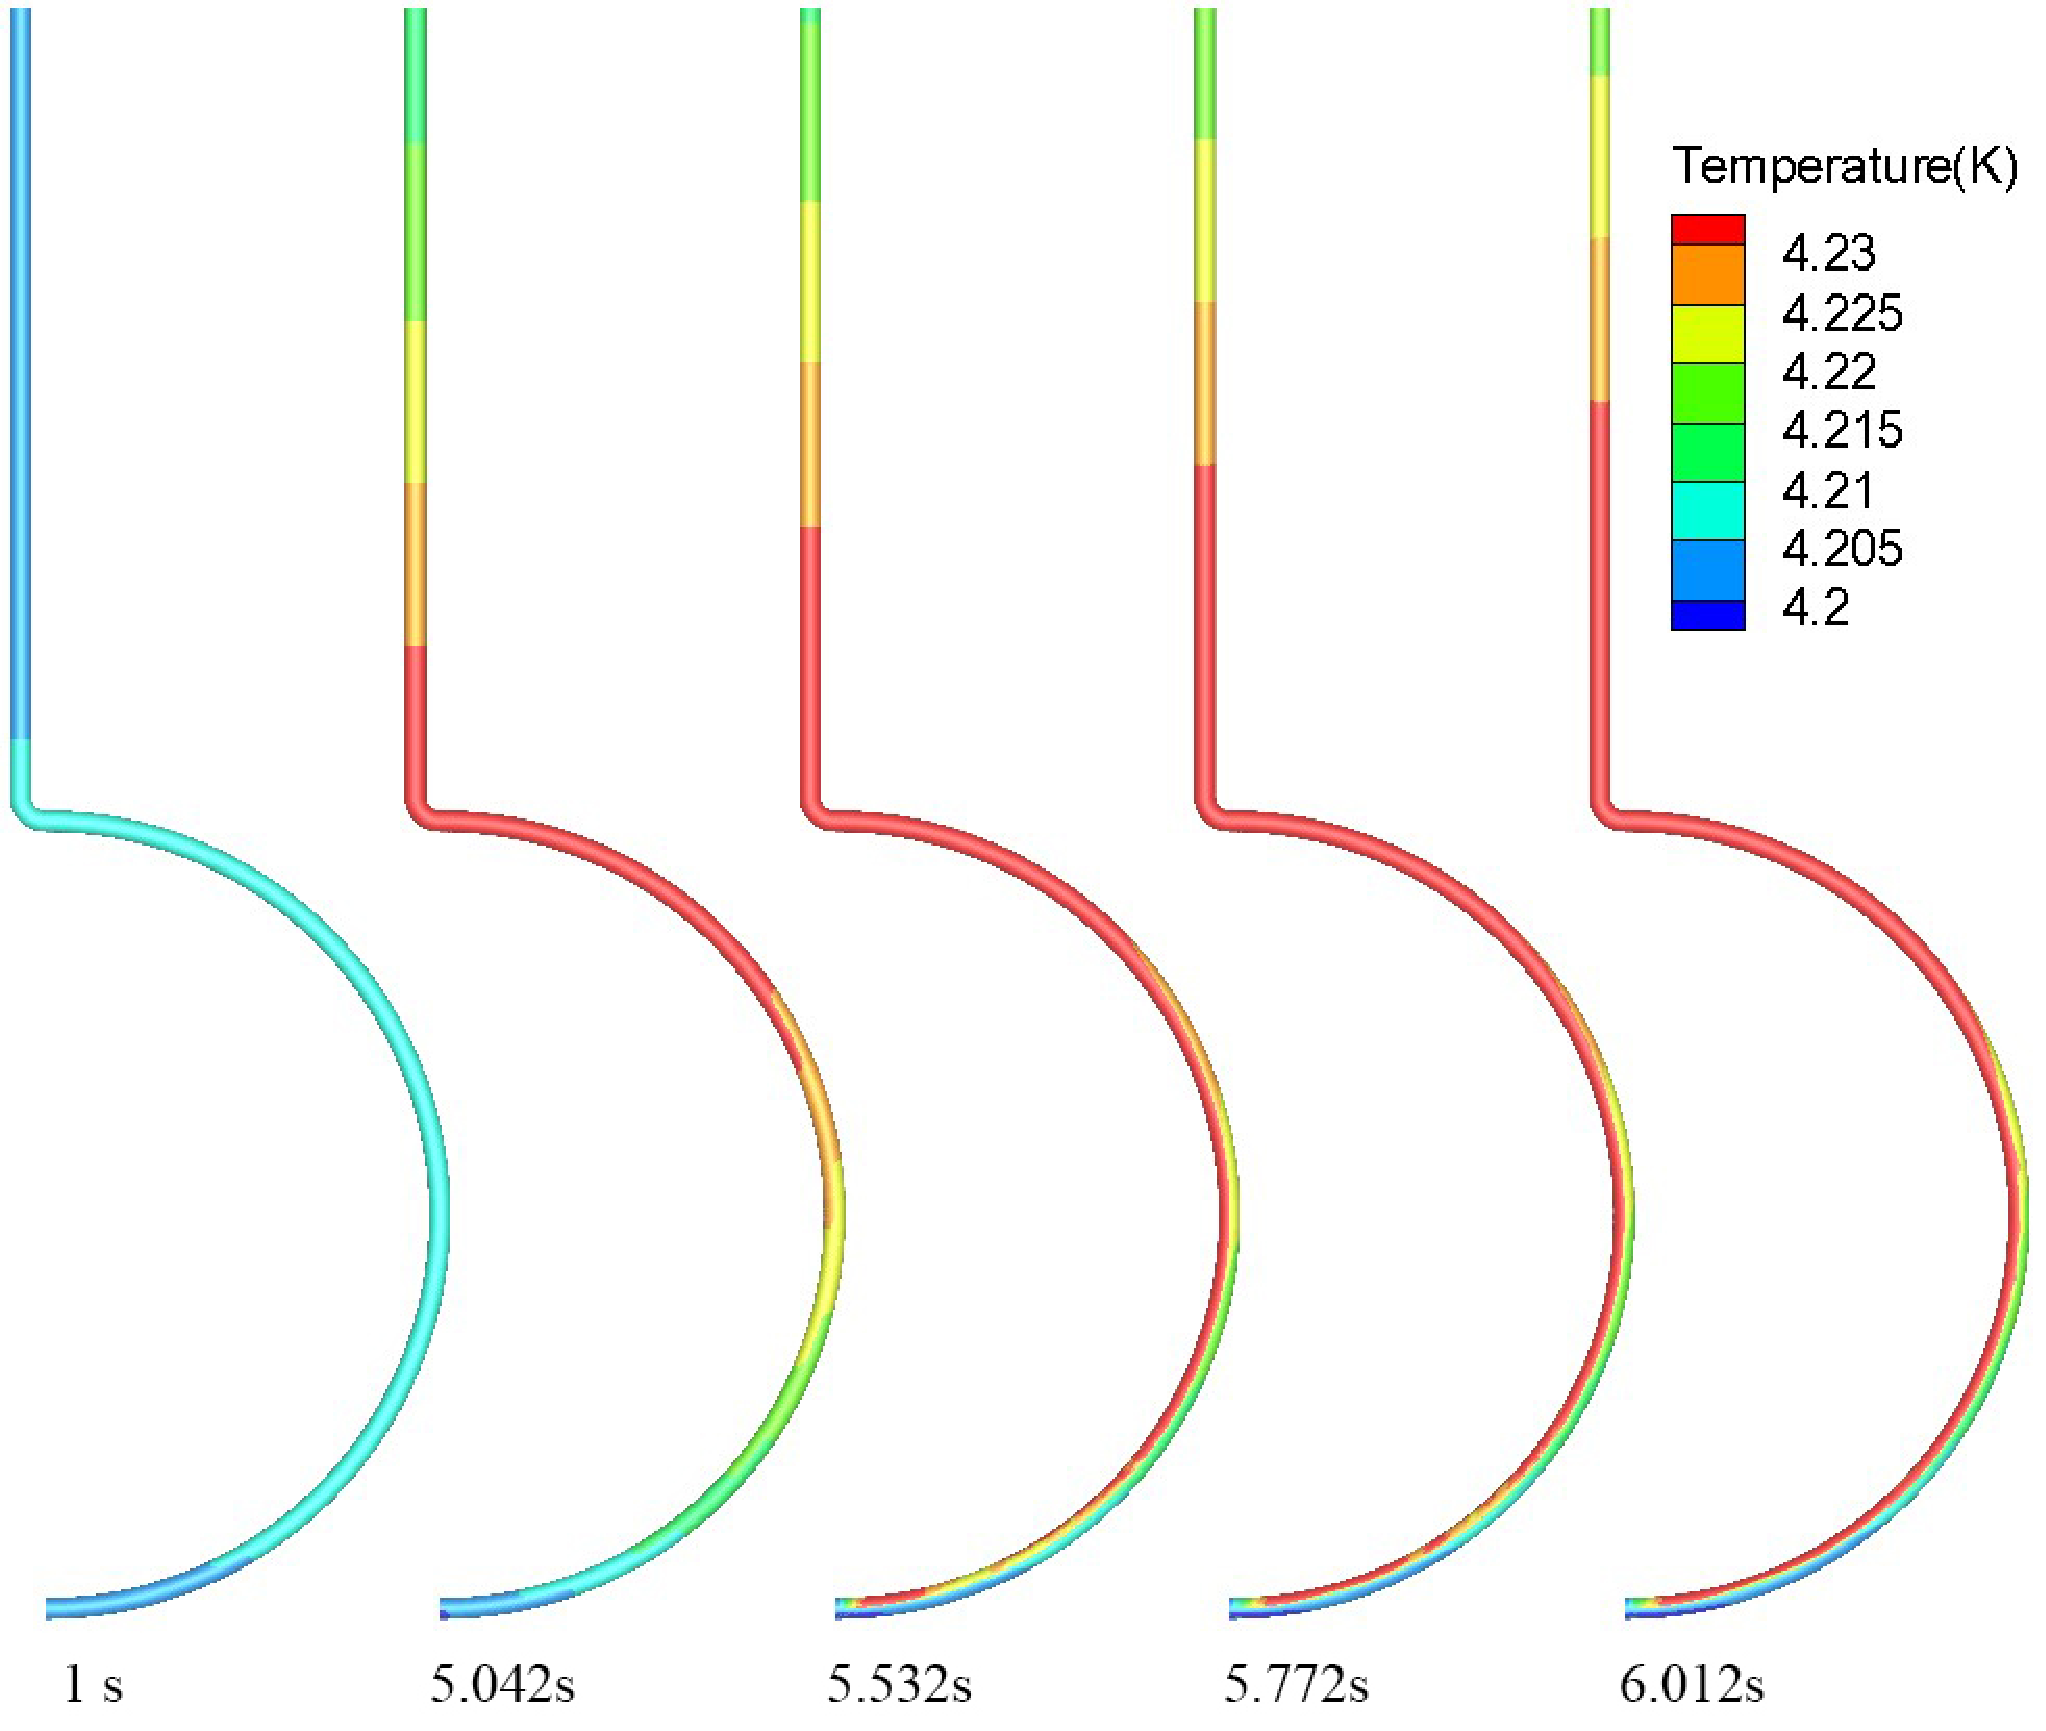
\includegraphics[scale=0.36]{Figures/Magnet/53}
\caption{The comparison of the temperature distribution}
\label{fig:53}
\end{figure}
\begin{figure}[h!]
\centering
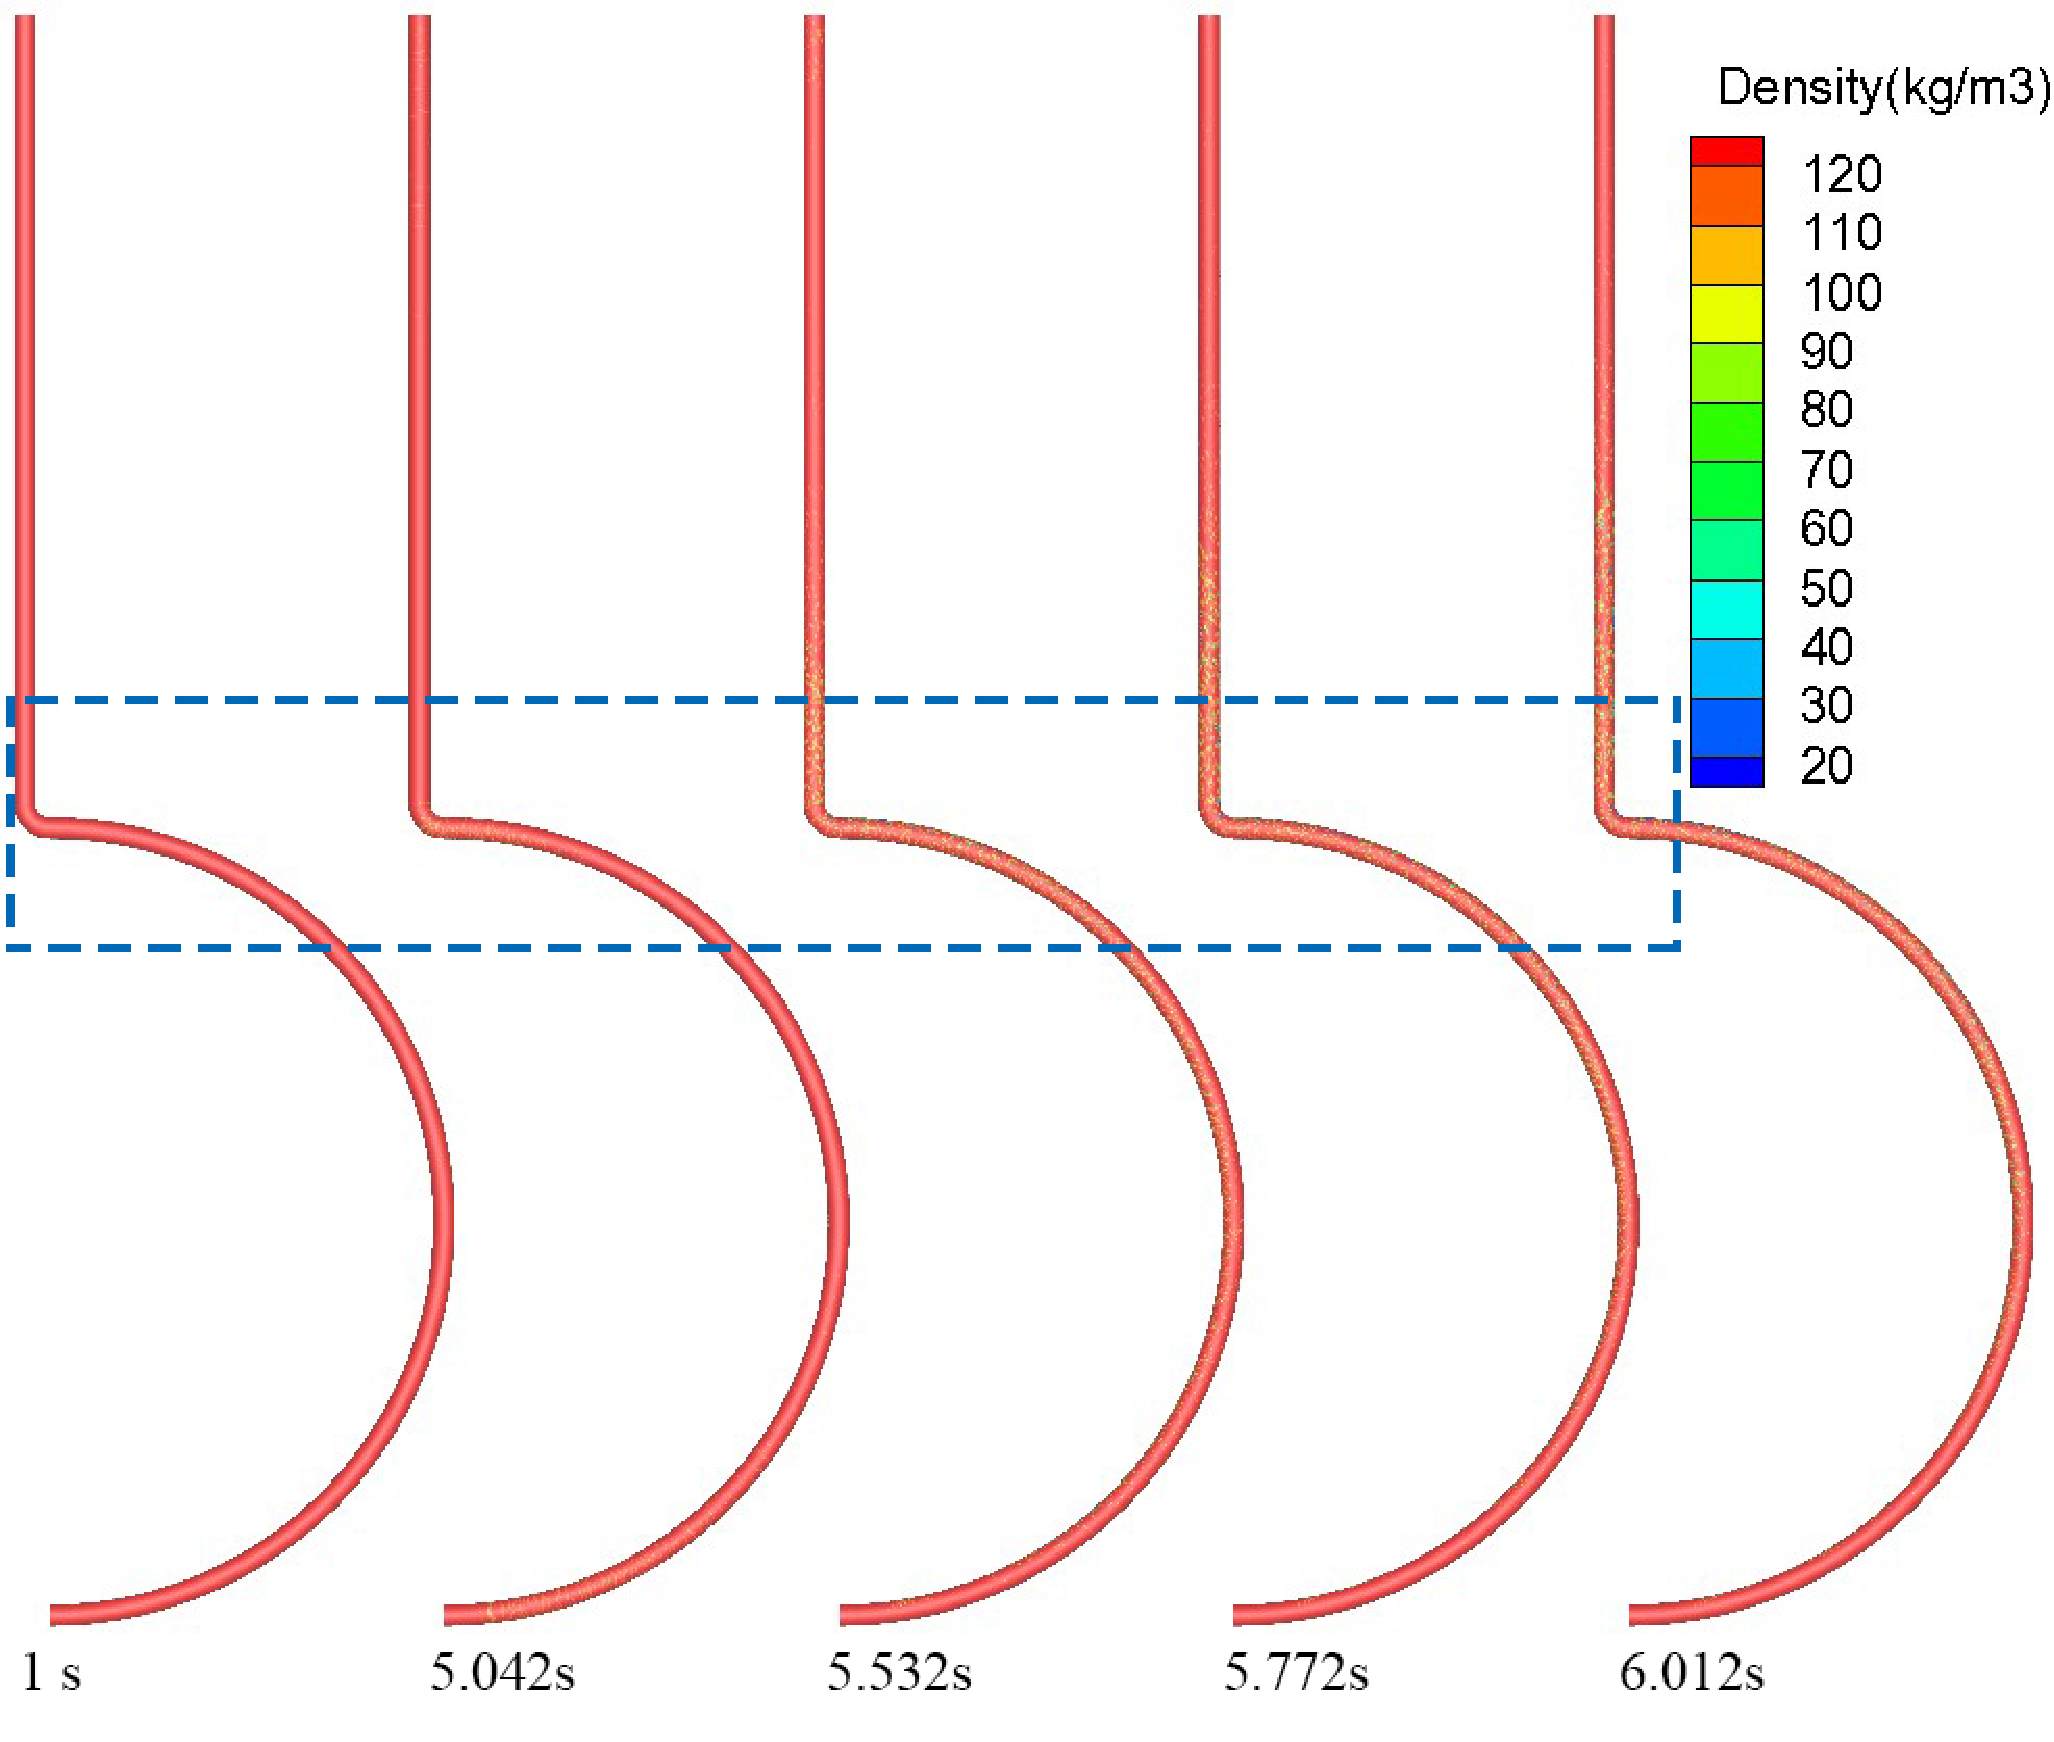
\includegraphics[scale=0.36]{Figures/Magnet/54}
\caption{The comparison of the density distribution. (red: liquid helium, blue: gas helium)}
\label{fig:54}
\end{figure}


Figure 6.5.5 shows the blue box part of Figure 6.5.4 (ie, the upper part of the cooling pipe). The helium bubbles emerged in the inner wall of the cooling pipe initially and then move outward because of the occurrence of buoyancy, part of the small bubbles gathered into a larger bubble in the vicinity of the outer wall, and followed to the outlet by the fluid.


\begin{figure}[h!]
\centering
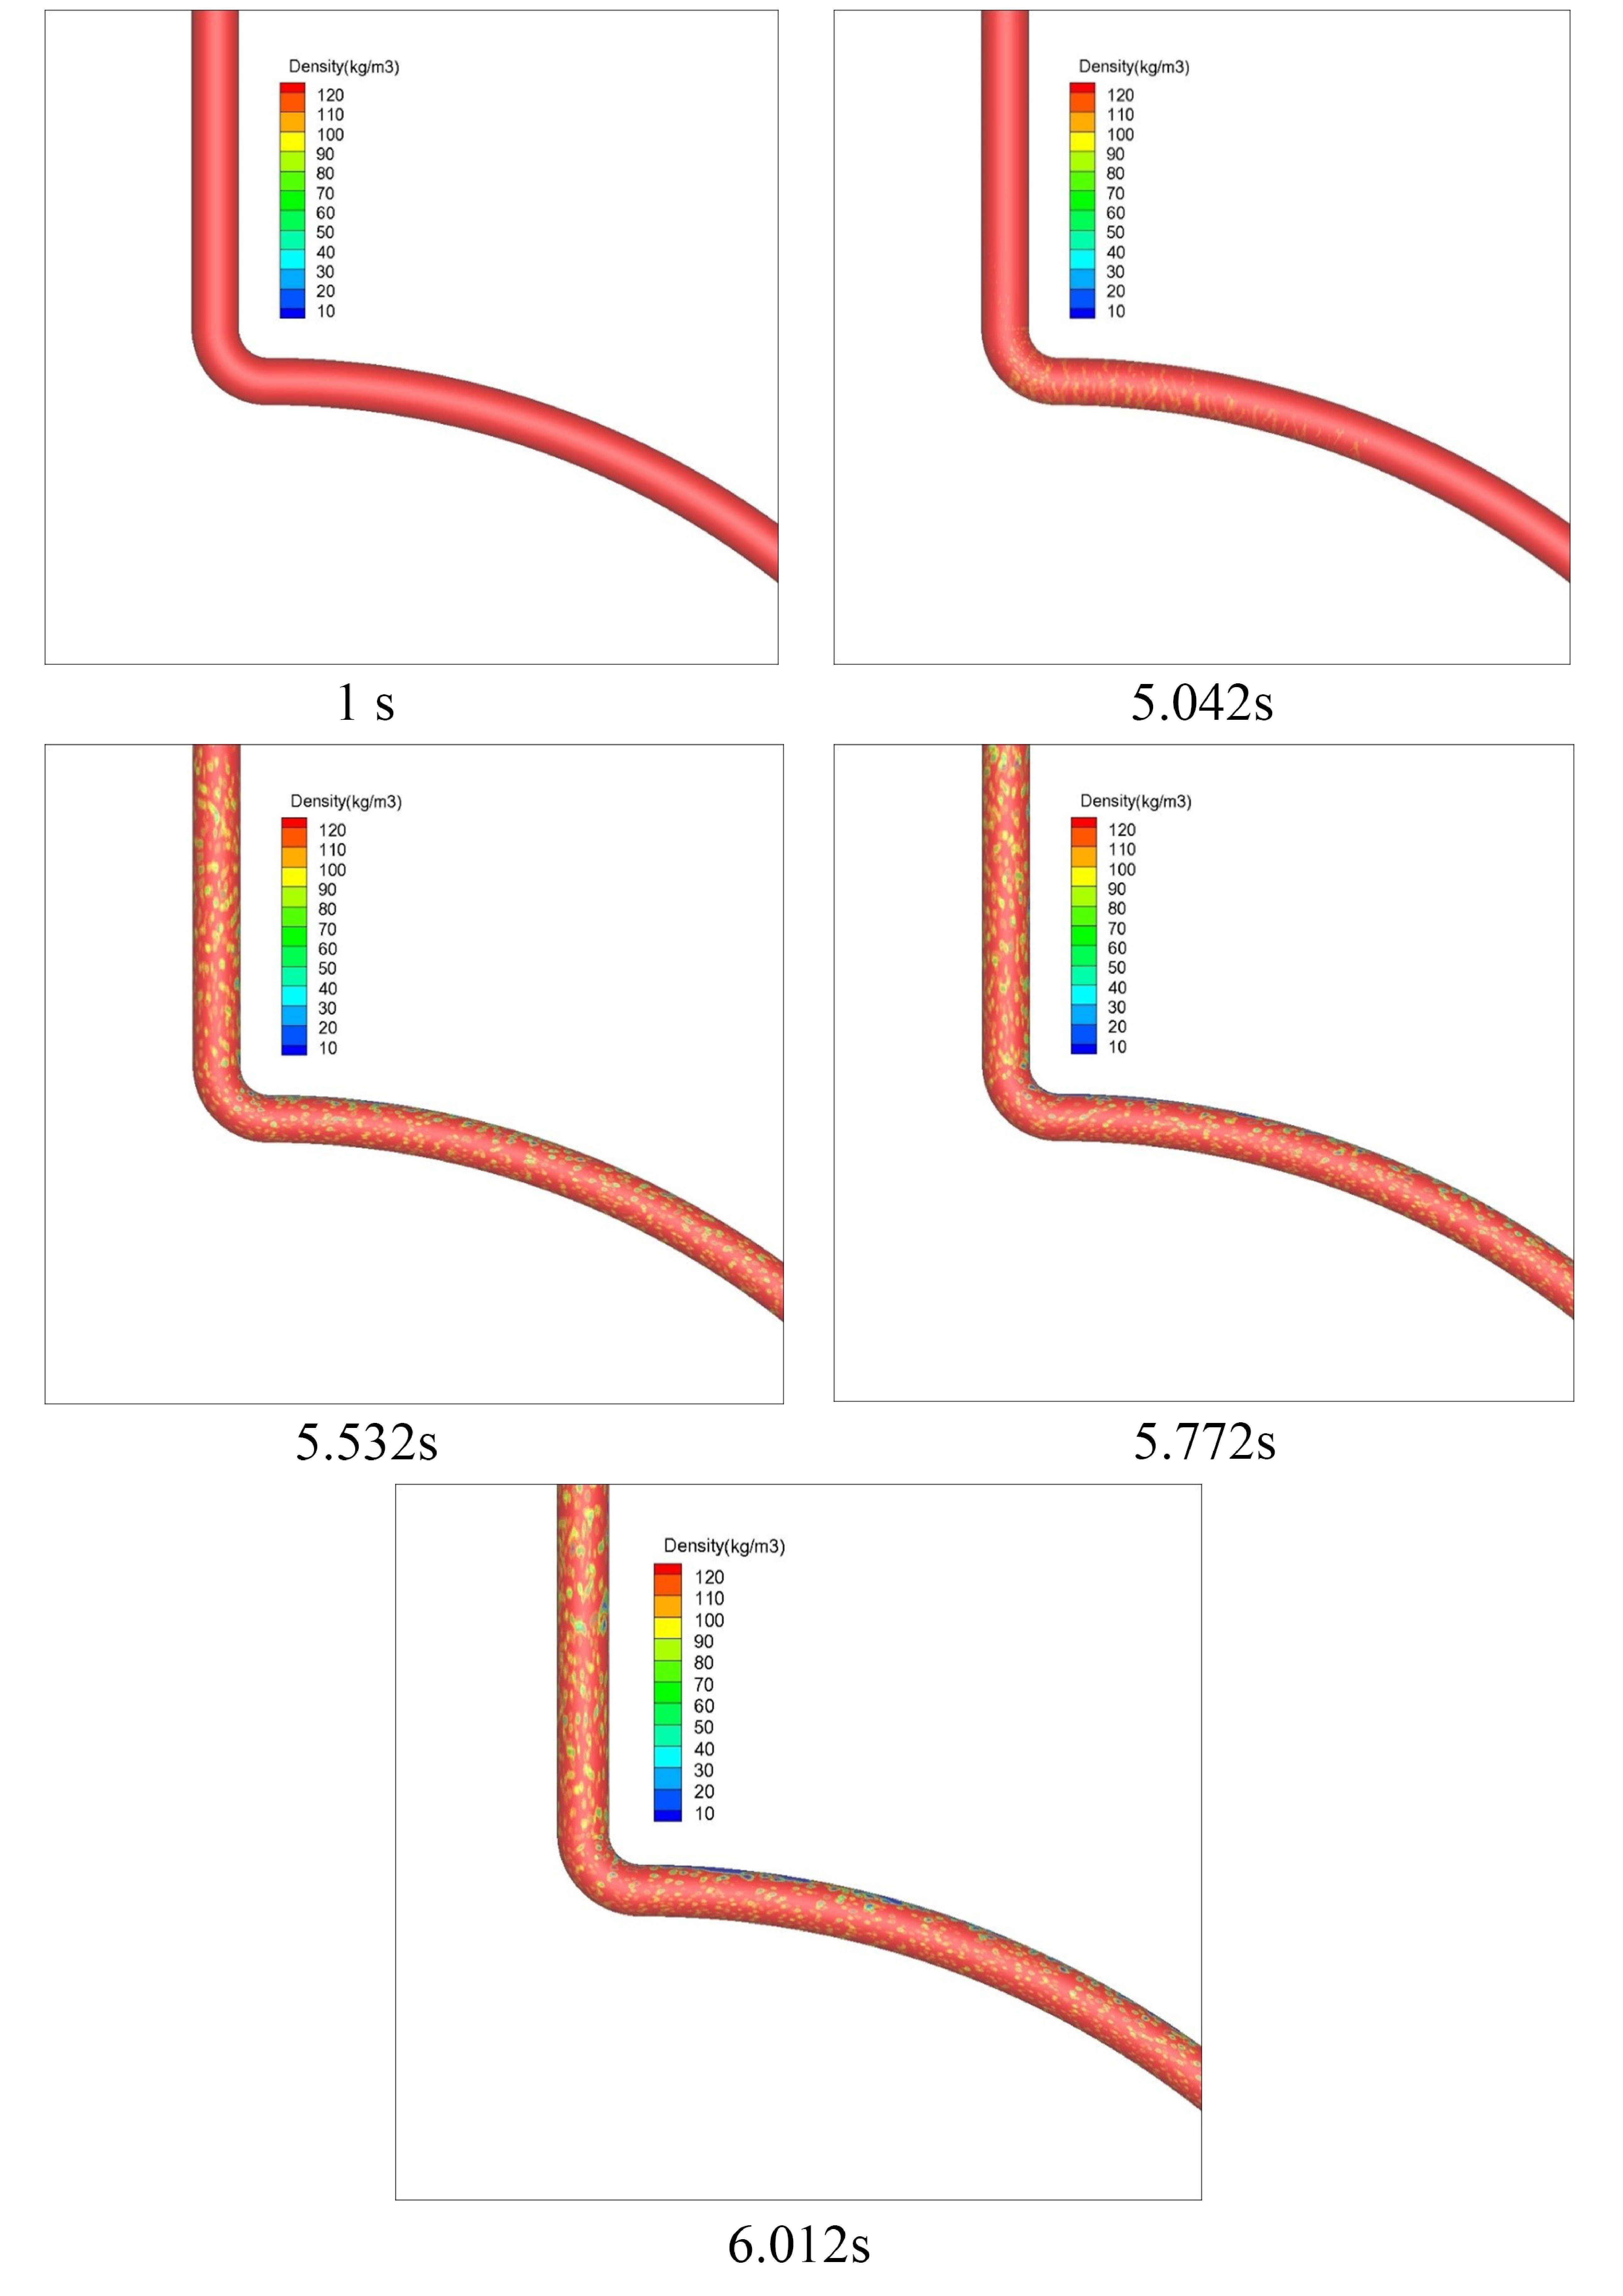
\includegraphics[scale=0.36]{Figures/Magnet/55}
\caption{The comparison of the density distribution in the upper part of cooling pipe. (red: liquid he,blue: gas he)}
\label{fig:55}
\end{figure}


\subsection{Experiment of a small-sized He thermosiphon }
\subsubsection{Experimental Set-up}


As shown in Figure 6.5.6, the experimental facility consists of a vertical oriented one meter long cryostat insulated by vacuum space and two cold shields which are conducted by cold head to minimize radiation and conduction heat transfer from the environment. The loop is mainly composed of two vertical tubes joined in a U shape with the upper ends connected to the phase separator, and the phase separator is connected directly to the second cold head. The cooling power is 1.0W@4.2K.


As shown in Figure 6.5.7,the schematic of experimental measures circulation loop. Five thermometers distributed along the tube were used for measurement of local inner wall temperature to deduce the corresponding heat transfer coefficient. The sensors have a measurement sensitivity of 0.1K between 2.5K to 25K.

\begin{figure}[h!]
\centering
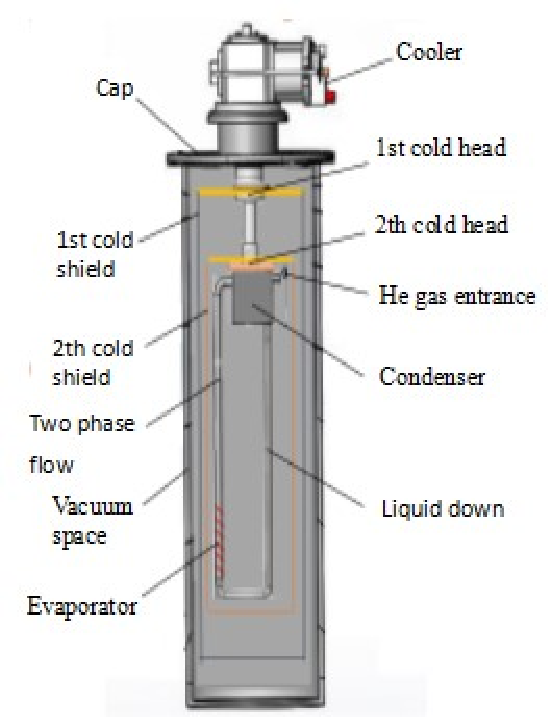
\includegraphics[scale=0.36]{Figures/Magnet/56}
\caption{the main component structure of the experimental cryostat}
\label{fig:56}
\end{figure}


\begin{figure}[h!]
\centering
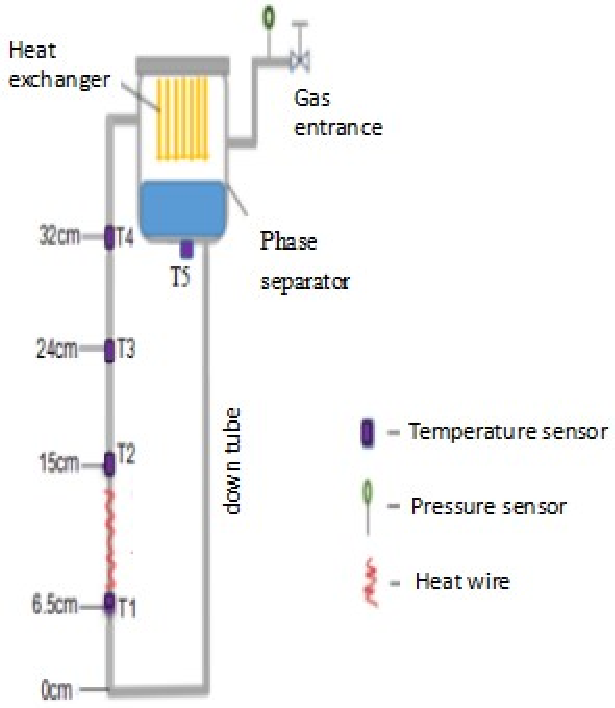
\includegraphics[scale=0.36]{Figures/Magnet/57}
\caption{Schematic of the experimental measures circulation loop}
\label{fig:57}
\end{figure}

\subsubsection{Experimental result and analysis}


As shown in Figure 6.5.8, when the heat flux is 137W/m2,the helium pressure increases from 0.3MPa to 1.8MPa,then descend to near 1.1MPa ,after that following up and down under the filling ratio of 26\%.When the filling ratio is 52\% and 87\%,the pressure in thermosiphon maintain constant in general,as for ratio 87\%,the pressure is a little higher than 52\%.


\begin{figure}[h!]
\centering
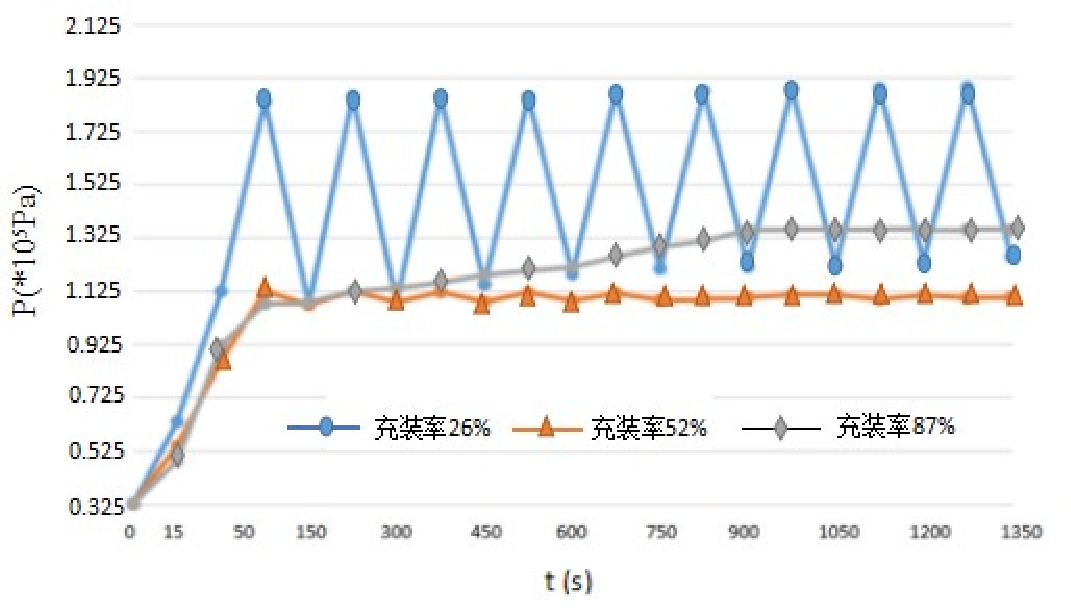
\includegraphics[scale=0.36]{Figures/Magnet/58}
\caption{ the saturation pressure of different filling ratio varies with time in heat flux $137W/m^2$}
\label{fig:58}
\end{figure}


In the beginning of the experiment,  $\Delta T_w$ increases linearly with heat flux at low heat fluxes. Before $q_A = 25W/m^2$ at point A on Figure 6.5.9, the heat transfer is identified as single phase natural convection. After point A, the temperature difference show difference between Figure 6.5.9 (a) and Figure 6.5.9 (b),the reason is that heat transfer intensity in exit section is higher than that in entrance, this leads to the upper comes to dry out earlier, then develop to the bottom with heat increase.
a) Before $q_A = 25W/m^2$ at point A, the heat transfer is identified as single phase natural convection.
b) Between points A and C is in the developing nucleate boiling regime.
c) The transition from nucleate boiling to film boiling occurs at point C.
d) After point E helium enters its supercritical state.


\begin{figure}[h!]
\centering
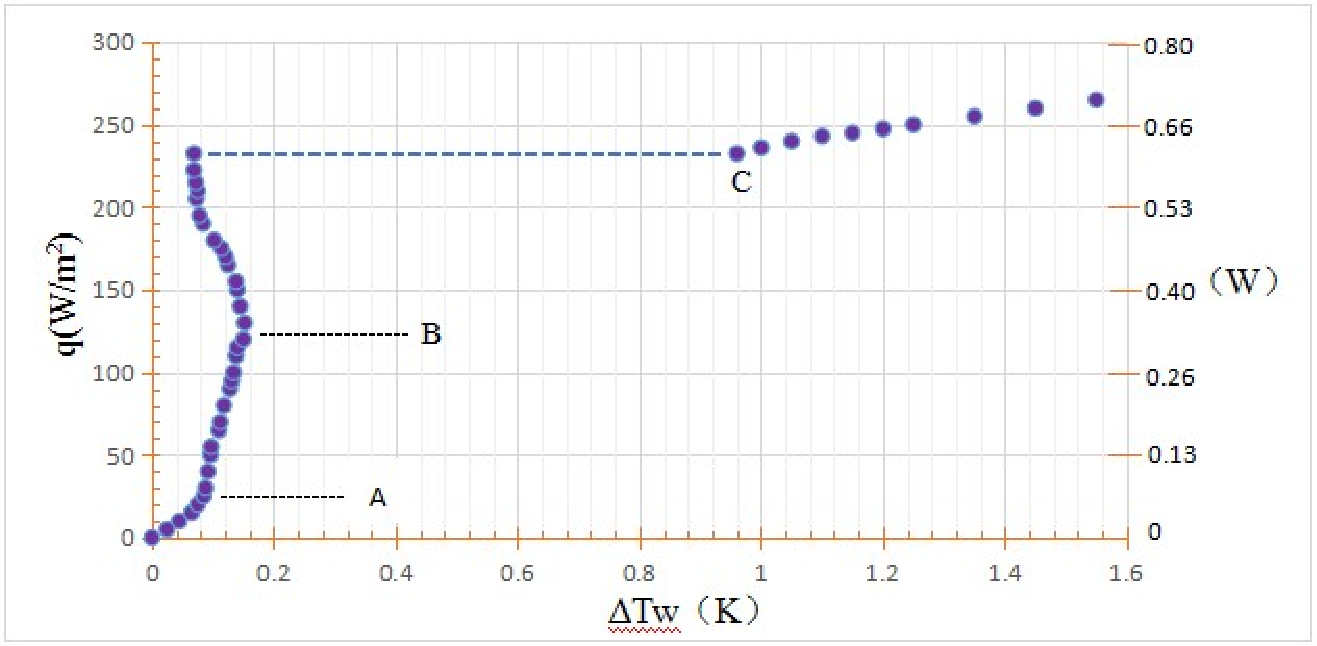
\includegraphics[scale=0.36]{Figures/Magnet/59a}
\caption{Boiling curve at $Z=6.5cm$ in the entrance}
\label{fig:59a}
\end{figure}

\begin{figure}[h!]
\centering
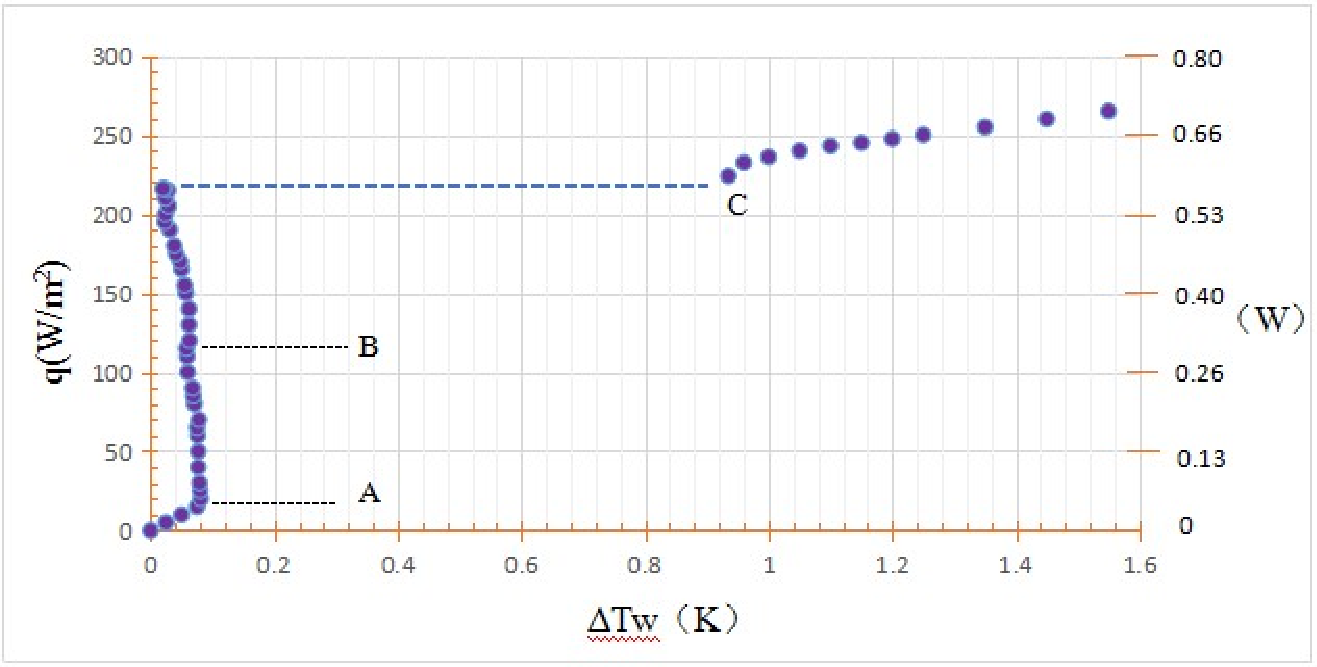
\includegraphics[scale=0.36]{Figures/Magnet/59b}
\caption{Boiling curve at $Z=32cm$ in the exit section}
\label{fig:59b}
\end{figure}
Calculation formula of heat transfer:
$$h=frac{q}{T_w-T_f}$$


Where $T_w$ and $T_f$ are, respectively, the wall and fluid temperatures, we assume $T_4=T_f$ .
a) h changes almost linearly with q in the whole regime, at location $z = 6.5 cm$.
b) The heat transfer is better in the upper part ($z<24 cm$) of the testing tube than the lower locations($z < 6.5 cm$) where boiling is less developed.
c) When the heat flux becomes higher than point C, heat transfer fall off quickly, since a large amount of vapor cannot be liquefied immediately, the heating surface is covered by a film of vapor.

\begin{figure}[h!]
\centering
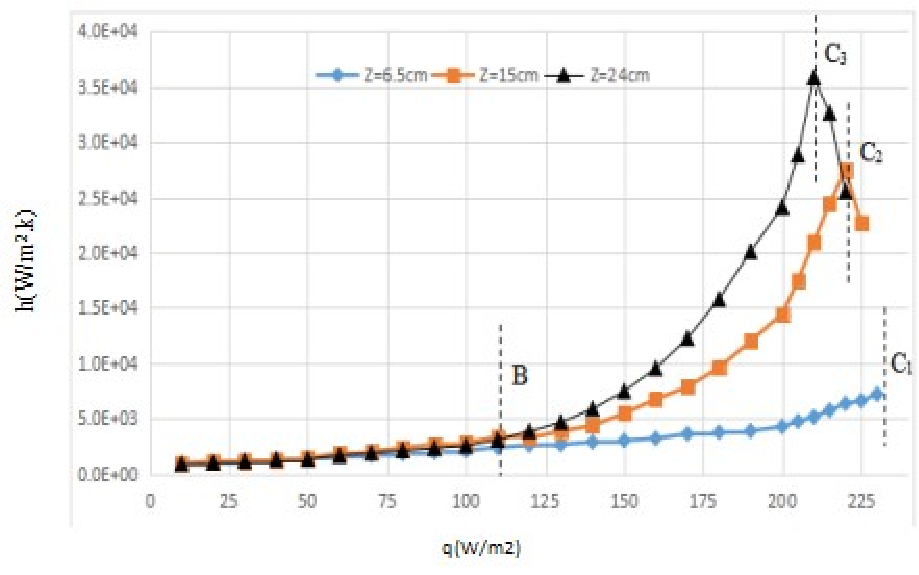
\includegraphics[scale=0.36]{Figures/Magnet/510}
\caption{ Heat transfer coefficient at different locations of the tube}
\label{fig:510}
\end{figure}


\subsection{Cryogenic Plant Design}
\subsubsection{ Refrigeration System}



The refrigeration system (Compressors, Cold box, Transfer lines, LHe5000L Dewar) has been designed in view of two main operation modes: cool-down from 300 K to 4.45 K and operation at 4.45 K. The refrigeration cycle is based on a modified Claude cycle.


The purpose of compressors is to provide the flow of gas at required pressures to achieve the performance of the refrigerator according to the cryogenic process.


The compression system consisted of two oil injected screw compressors, which nominal mass-flow is about 180 g/s. The maximum pressure level is expected to be 18 bar. The third screw compressor with a capacity limited to 40 g/s was used for the recovery of helium gas from the magnet, when the main cryogenic plant would be shut down. This gas will be compressed and stored without polluted and thus can be reusable after the shut-down. To avoid the oil enter the cryogenic system, the complete oil removal and purifier system would be needed for the operation of the screw compressors. The helium will be stored at the surface outdoors in two 250-m3 cylinders at 20 bara. This storage capacity provides a supply of two full loads for the refrigeration plant and the magnet system. A 50 000 l liquid nitrogen dewar for pre-cooling the magnet in the temperature range 300 to 100 K is also located at the surface. During this cooling phase, the expected liquid nitrogen mass-flow is 500 l/h.


Cold Box comprises cryogenic heat exchangers, turbine expanders, cryogenic absorbers, valves, instrumentation, vacuum unit and control panel etc.


On the base of the thermal loads of the superconducting magnet system and of the operating conditions, a refrigerator would be used with a power rating of $1.5 kW @ 4.5 K$ (entropic equivalent).


The upper part of the cold box contains a set of liquid nitrogen/helium heat exchangers for magnet cooling down to 100 K. In addition the liquid nitrogen pre-cooling would increase the helium liquefaction of the plant when necessary. The cold box will be connected to the magnet via an intermediate cryostat (shown as Fig. 6.5.1), which will house all the cryogenic valves needed to pre-cool the magnet and its heat shield. Cryostats are technical systems that maintain equipment or cryogenic liquids at cryogenic temperatures. As such, they are one of the fundamental building blocks of cryogenic systems. The intermediate cryostat includes a 5000 l reserve of liquid helium to allow the magnet slow discharge in the event of failure of the cryogenic system or other facilities.


The cold box will be connected to the intermediate cryostat by a single thermally shielded transfer line containing 4 separate lines. Two for the magnet circuit helium, and two for the heat shield circuit. The cryostat will be connected to the valve box and helium phase separator by means of 4 separate transfer lines.


The magnet's heat shield will be cooled by tapping off the required mass-flow at the level of the outlet of the first turbine expander and be reinjected the shield return at the inlet to the second turbine expander.


The magnet's vacuum insulation will be done by a primary pumping station consisting of two vane pumps and two 900 m3/h Roots pumps. These will be installed in the service cavern and connected by a 300 mm diameter pipe to the distribution pumps described below. A diffusion pumping station also connected to the vacuum chamber of the magnet. One 8000 l/s diffusion pump will be directly connected by a 600 mm spool piece to the vacuum chimney (400 x 800 mm2). A second 2000 l/s pump will be directly connected to the vacuum chamber of the magnet's valve box.

\subsubsection{Cryogenic flow-sheet and Operation mode}


There are six operating modes for the cryogenic system, which detailed descriptions are as follows. The schematically flow sheet of the cryogenic equipment is shown in Figure 6.5.11.
Cooling-down phase from 300K to 100K


The magnet will be pre-cooled using the liquid nitrogen/helium heat exchanger in the cold box (Shown as Fig. 1). To transport all the helium mass-flow of the screw compressors, both the valve box and the intermediate cryostat have a bypass. Valves V271, V272, V273 will be closed and valves V260, V290 open. By-pass V3 in the valve box will be used to allow the necessary mass-flow. The gas return from the magnet will be channeled inside the cold box to the appropriate temperature level. During this phase the expansion turbines are switched off and cooling of the heat shield has not yet started.
Final cooling-down phase from 100K to 4.5K


The cold box expansion turbines are in operation. Circulation in the magnet heat shield starts and in parallel a minimal mass-flow of 80 g/s is maintained in the circuits of the coil. At the same time, part of the main mass-flow is tapped off to cool the intermediate cryostat and the 5000 l liquid helium dewar.
Normal operation at 4.5K


The cold box with its own phase separator, upstream of V260, will supply the supercritical liquid helium at 3bara to the 5000 l cryostat. V271 will allow the level of liquid helium in the dewar to be regulated. The pressure of the cryostat will be set at 1.5 by V273, located at the cold return to the cold box. Transfer to the magnet valve box and phase separator will be done by the supply valve V272. The shield will be cooled via valves V280 and V281 with a helium mass-flow of 35 g/s, at an input temperature of 60 K and an output temperature of 80 K. The input pressure will be 5 bara and the pressure drop lower than or equal to 150 mbar.
Operation at 4.5K without cold box and with or without compression system


In case of failure of the refrigerating system, the dewar continues to supply liquid helium to the phase separator of the valve box. The 5000 l capacity will ensure the supply of liquid helium to the magnet throughout the current slow discharge phase which takes approximately 4 hours. With the expansion turbines out of operation the heat shield is no longer cooled. After depressurisation of the shield circuits from the nominal operating pressure, the V7 by-pass valve conveys the flow evaporated by the magnet into the circuits of the heat shield. The evaporation rate of the magnet will be 20 g/s and the total expected pressure drop in the shield circuits is less than 120 mbar.


If the compressors for the cryogenic cycle are operating, the helium from solenoid return and current leads may be recovered and stored in the gas holders. These flows will be injected at the low pressure level of the main compression system. In the event of total shutdown, including that of the cycle compressors, these flows will be recovered and stored by the recovery compressor, which must be connected to the auxiliary external safety services allowing its operation in the event of the main facilities failure. Valve V283 controls the pressure in the phase separator of the magnet when the cold box is not in operation and the heat shield during depressurisation.

Fast energy dump


Valves V1 and V3 are closed and the expansion turbines are shut down. The cold box is isolated by valves V260 and V290, as is the 5000 l dewar by its valves. The cryostat has its own exhaust through V275 via a heat exchanger to the low pressure of the compression system.
The "thermosiphon" circuit is depressurised by the V7 by-pass valve through the shield.
Two options are being considered for thermal recovery of the magnet from the average temperature of 50 K reached after a fast energy dump. As there are no valves on the thermosiphon return, cooling may be done either by controlling the opening of the by-pass of the Joule-Thomson in the cold box so as to limit the pressure rise in the low-pressure circuit, or by supplying the magnet directly with liquid helium from the cryostat's 5000 l reserve.

Warming-up of the magnet


During shutdowns, it is agreed that the magnet will be electrically reheated and decoupled from the cryogenic circuits to allow maintenance of the compressors, the refrigerator and auxiliary equipment.

\begin{figure}[h!]
\centering
\includegraphics[scale=0.36]{Figures/Magnet/511}
\caption{Schematical flow sheet of the cryogenic equipment}
\label{fig:511}
\end{figure}





\section{Quench Protection and Power supply}
\subsection{ power supply}
The power supply for the solenoid is DC stabilized current supply with low voltage and high current, which should be adjusted slowly and evenly. In order to have a steady field, the ripple of the power supply should be lower. It is provided with a free-wheel diode systems and needs demineralized water cooling.
\begin{figure}[h!]
\centering
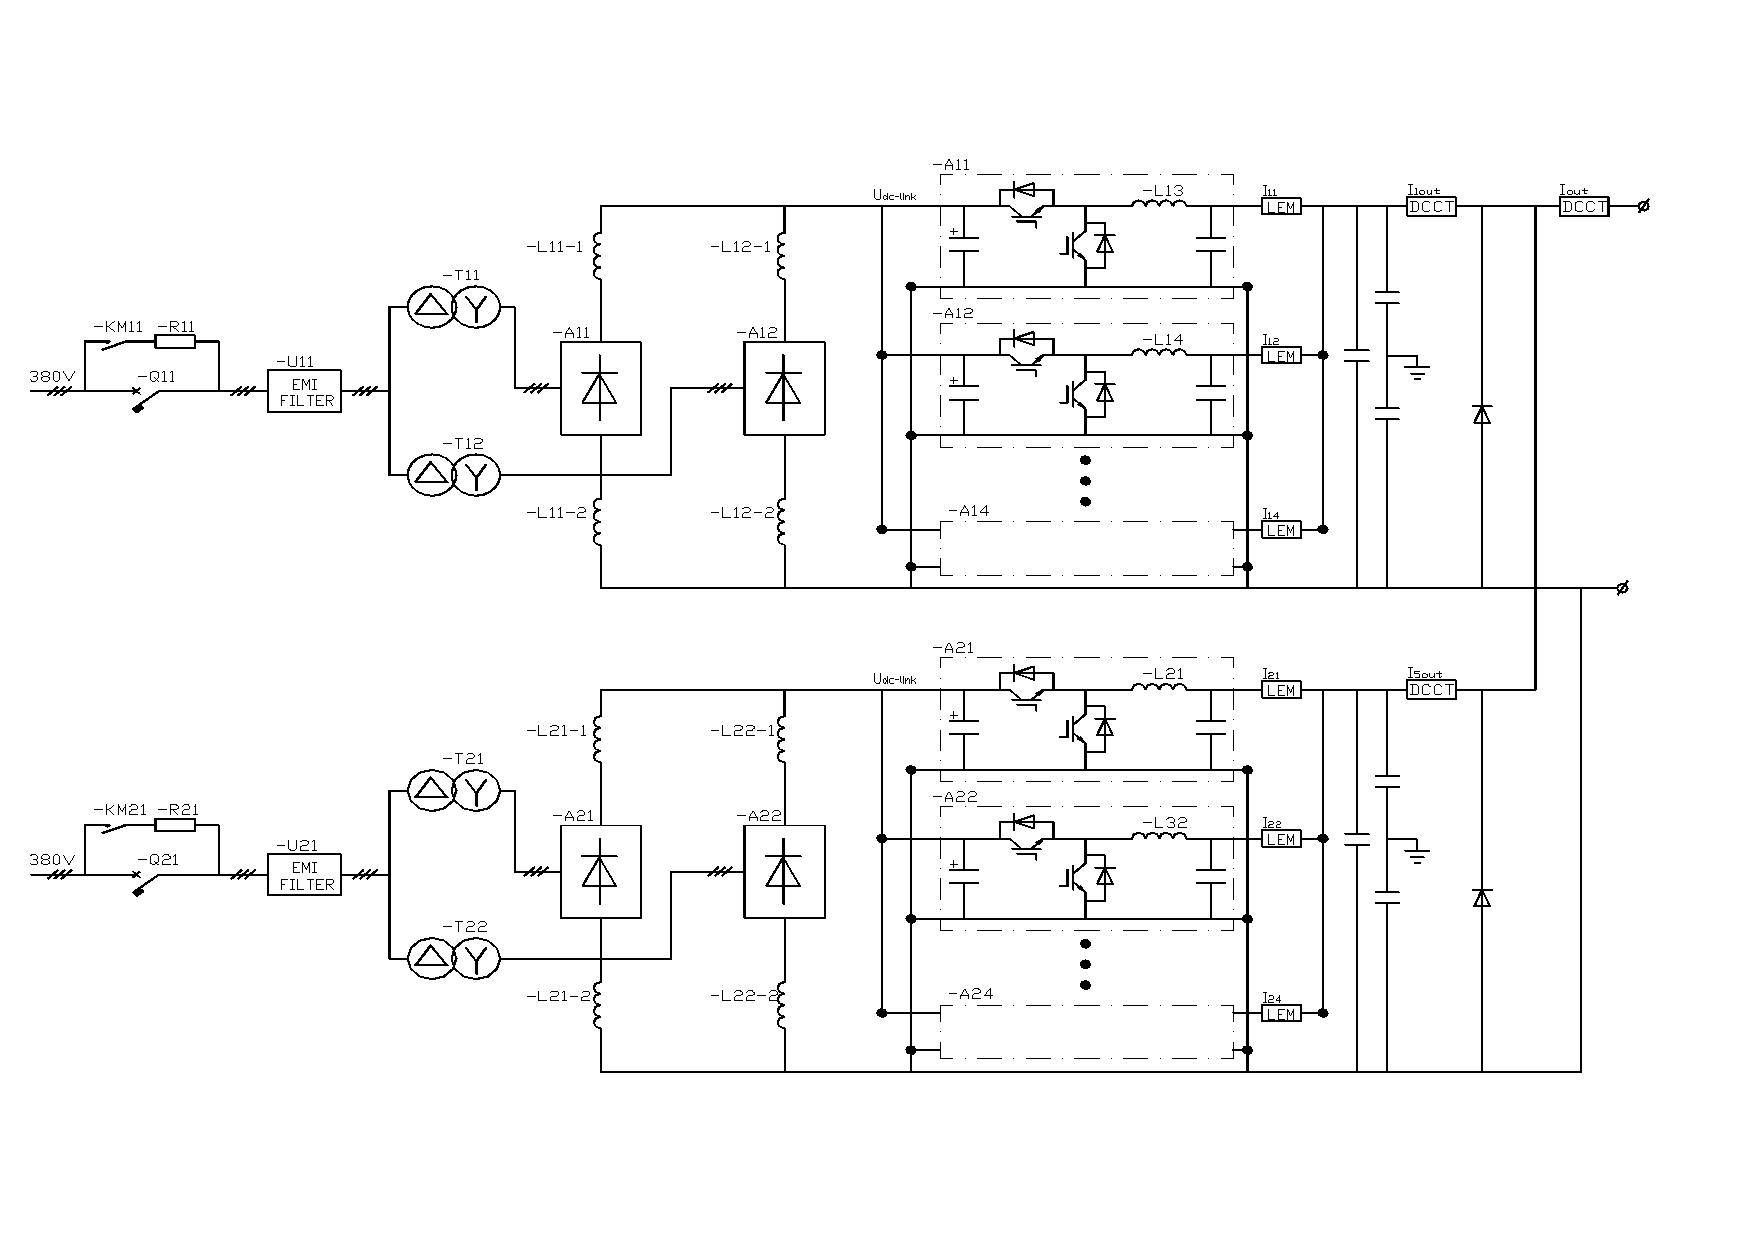
\includegraphics[scale=0.36]{Figures/Magnet/61}
\caption{Main circuit topology diagram}
\label{fig:61}
\end{figure}

The system consists of 2 stage 12 pulse diode parallel rectifier + post stage 4 group IGBT chopper circuit in parallel, in the post stage chopper circuit, the IGBT switching frequency is 10kHz, and the output power is 80kHz by phase shift frequency doubling control. In parallel chopper circuit, there is current sharing loop, plus balanced filter inductance, EMI filter is added to the power input to effectively reduce the pollution of the power supply to the grid. The main circuit uses the laminated busbar design process, reduce the circuit stray inductance, weaken the skin effect and proximity effect of high-frequency current.

\begin{figure}[h!]
\centering
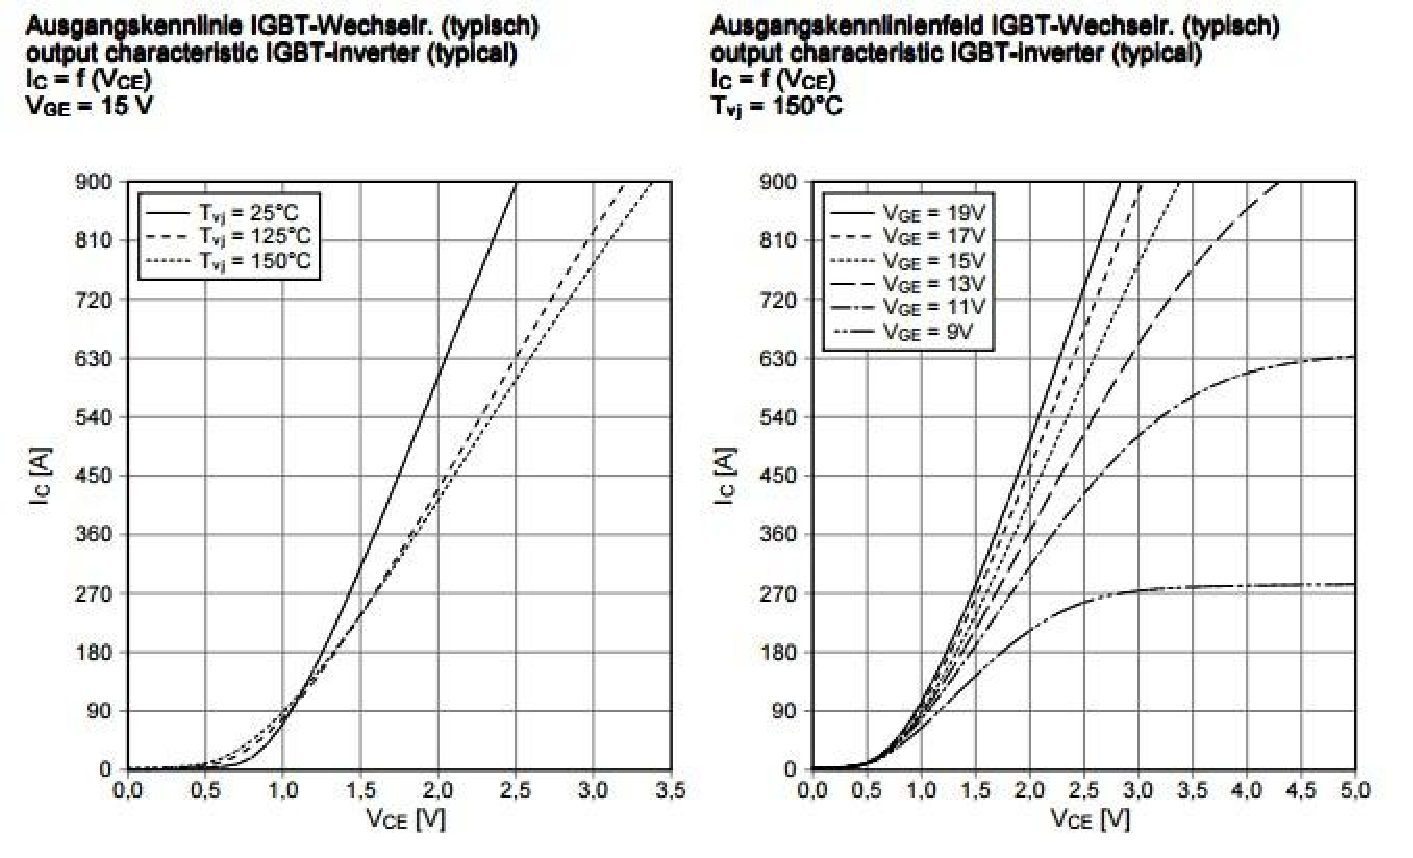
\includegraphics[scale=0.36]{Figures/Magnet/62}
\label{fig:62}
\end{figure}

\begin{figure}[h!]
\centering
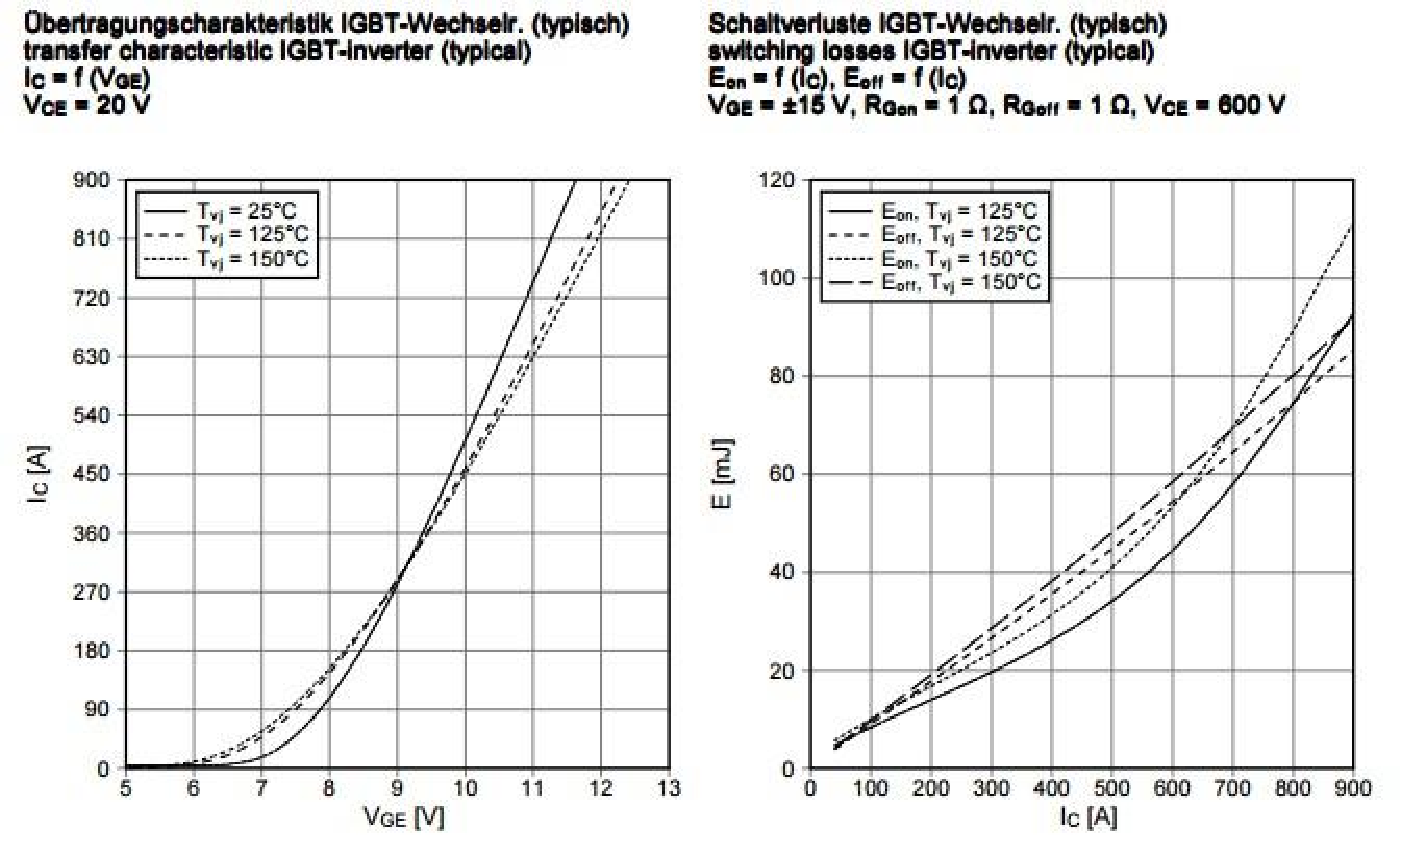
\includegraphics[scale=0.36]{Figures/Magnet/63}
\caption{IGBT Performance schematic diagram}
\label{fig:63}
\end{figure}


\subsection{control and safety systems}
The safety system and the control system are independent, but exchange information between each other.
The safety system measures magnet status in order to prevent operation in dangerous condition. The safety signals coming from quench detectors and voltage taps are transferred to the main switch in the circuit directly and trigger a fast discharge of the magnet. Also the quench detectors are used to protect the bus bars and the current leads. In addition, a substantial amount of instrumentation is required to monitor the operational status of the magnet and to provide diagnostic data such as temperature, stress, position and etc.
The control system provides the controls needed to execute the automatic processes of the various running mode of the magnet system. It is based on PLC and control software.

Quench protection
Plan: to provide quench protection system for cepc magnet, including signal acquisition, quench judgment,Energy release device.
Pre research content: Design quench protection system, including design of quench detector, quench protectionCircuit, write out judgment program, investigate energy release device, including water cooling part.

Magnet parameter monitoring
Plan: monitoring the magnet parameters, radial and axial rod, low temperature, vacuum, bus
Temperature, valve box temperature and vacuum, power supply parameters monitoring, including current, voltage,Internal temperature, cooling water flow, etc..
Pre research content: because the monitoring parameters are mainly weak voltage and small current, multi-channel instrument is investigatedTables and PLC acquisition signals, design optimization collection program and program design
Meter.




\section{Iron Yoke Design}


According to the physical design, the CEPC detector solenoid magnet need to provide a 3.0 T field for precise trajectory measurement for charged particles. The CEPC solenoid consists mainly of three parts, which are a superconducting coil, a vacuum tank with a thermal shield and a magnet yoke. Fig. 1 shows the structure of the CEPC detector solenoid magnet and yoke. The solenoid magnet will produce an axial field and the magnet yoke will take responsible for the return of the magnetic flux and reducing the outside stray field to an acceptable level. At the same time, the magnet yoke must match several other design requirements. Firstly, the yoke will provide mechanical support for sub-detectors so that they can be positioned accurately. Secondly, the yoke will provide room for muon detectors which will be set between layer and layer of yoke. Thirdly, the yoke will provide space for data cable, cooling pipes and gas pipes and so on. According to the general design of the CEPC detector, the magnet yoke is divided into a cylindrical barrel and two endcap yokes. Taking into account of both mechanical performance and magnetic requirements, maybe high permeability material need to be developed as the yoke material. Preliminary design of the yoke will be described as following.
\begin{figure}[h!]
\centering
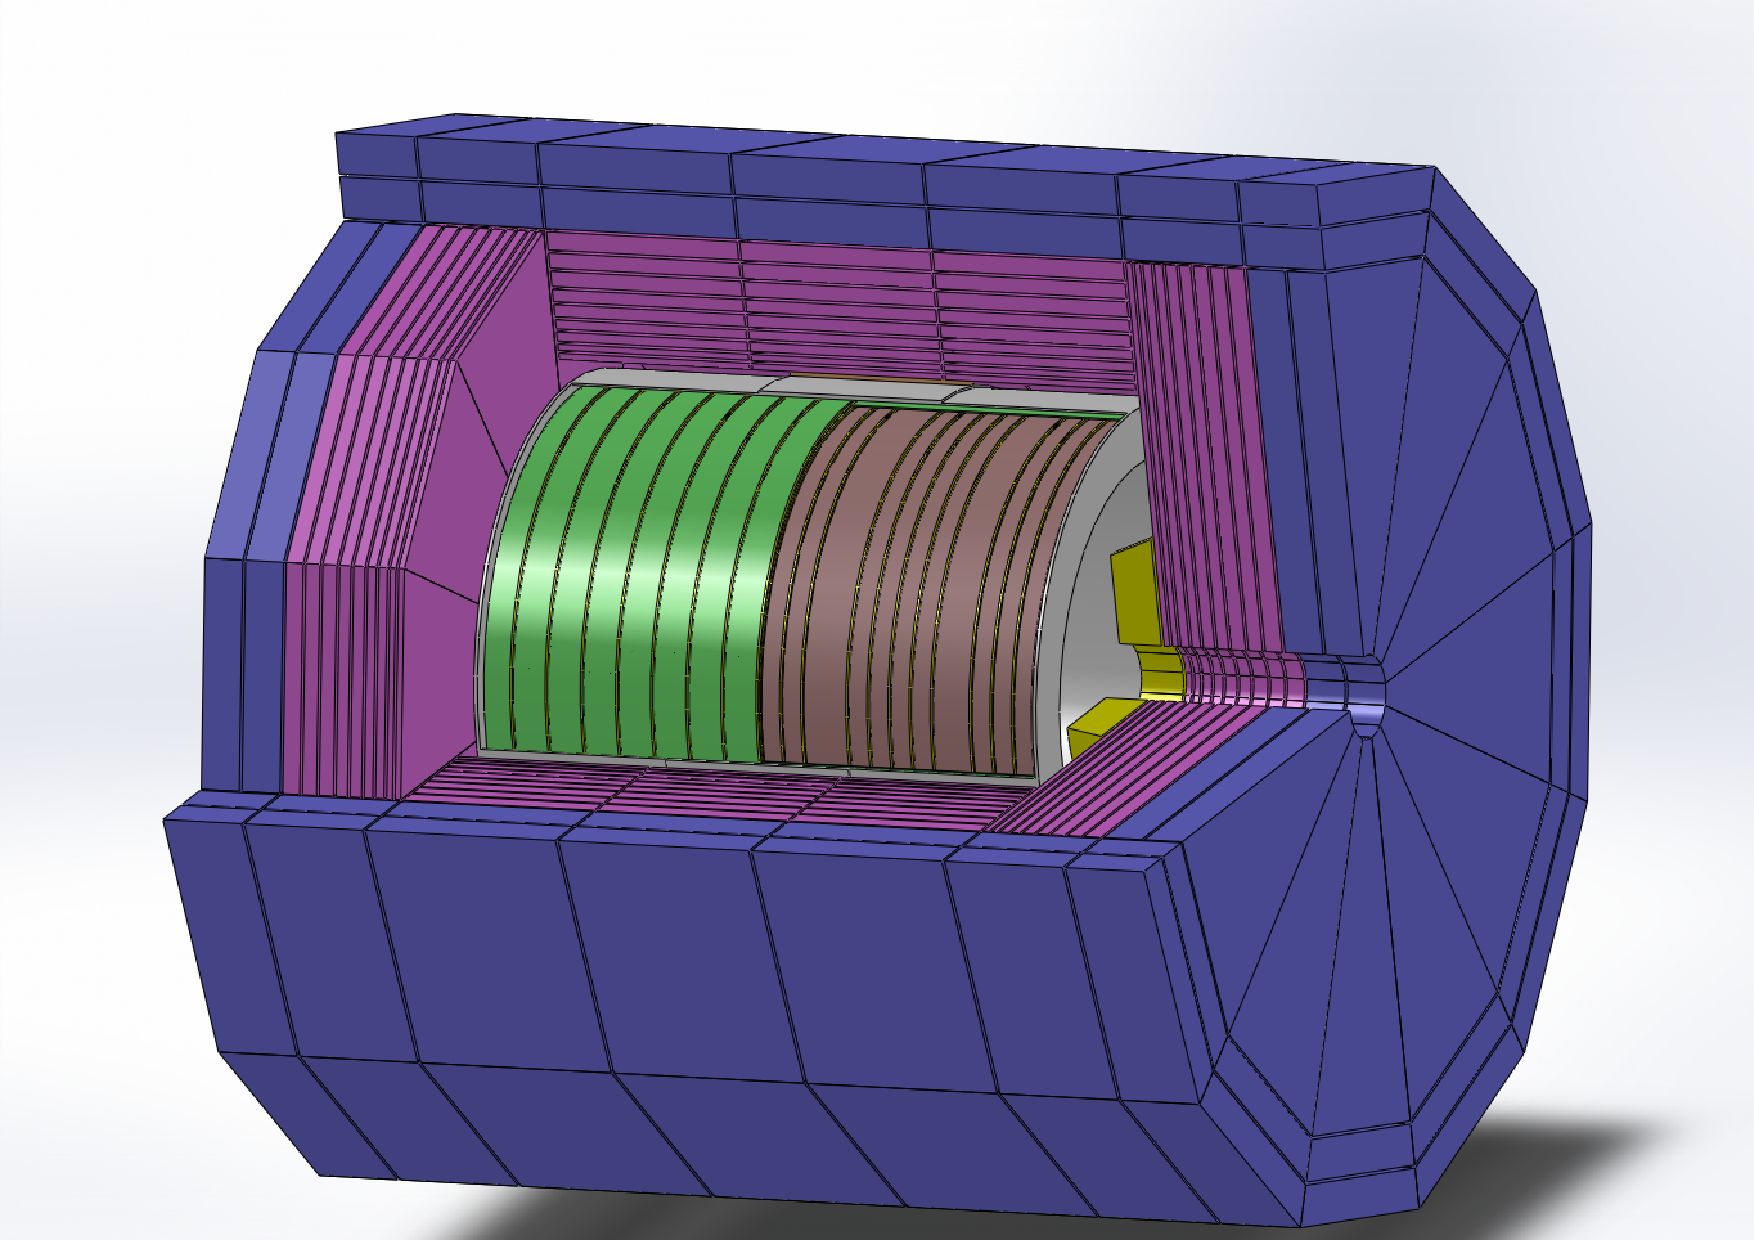
\includegraphics[scale=0.36]{Figures/Magnet/71}
\caption{iron and magnet}
\label{fig:71}
\end{figure}


\subsection{The Barrel Yoke}


The barrel yoke will have a length of about 8200 mm and with a dodecagonal shape. The inscribed circle diameter of the outer dodecagon will be about 13300 mm, and the inscribed circle diameter of the inner dodecagonal will be about 7800 mm. The barrel yoke will be composed of 3 rings, each ring will consist of 7 layers. There will be two 100 mm gaps between the rings which are designed to supply space for the data cables and services. The thickness of inner 4 layers are 100 mm and outer 3 layers are 450 mm. There will be 100 mm space between layers for muon detector. Fig. 2 shows the schematic design of the barrel yoke.

\begin{figure}[h!]
\centering
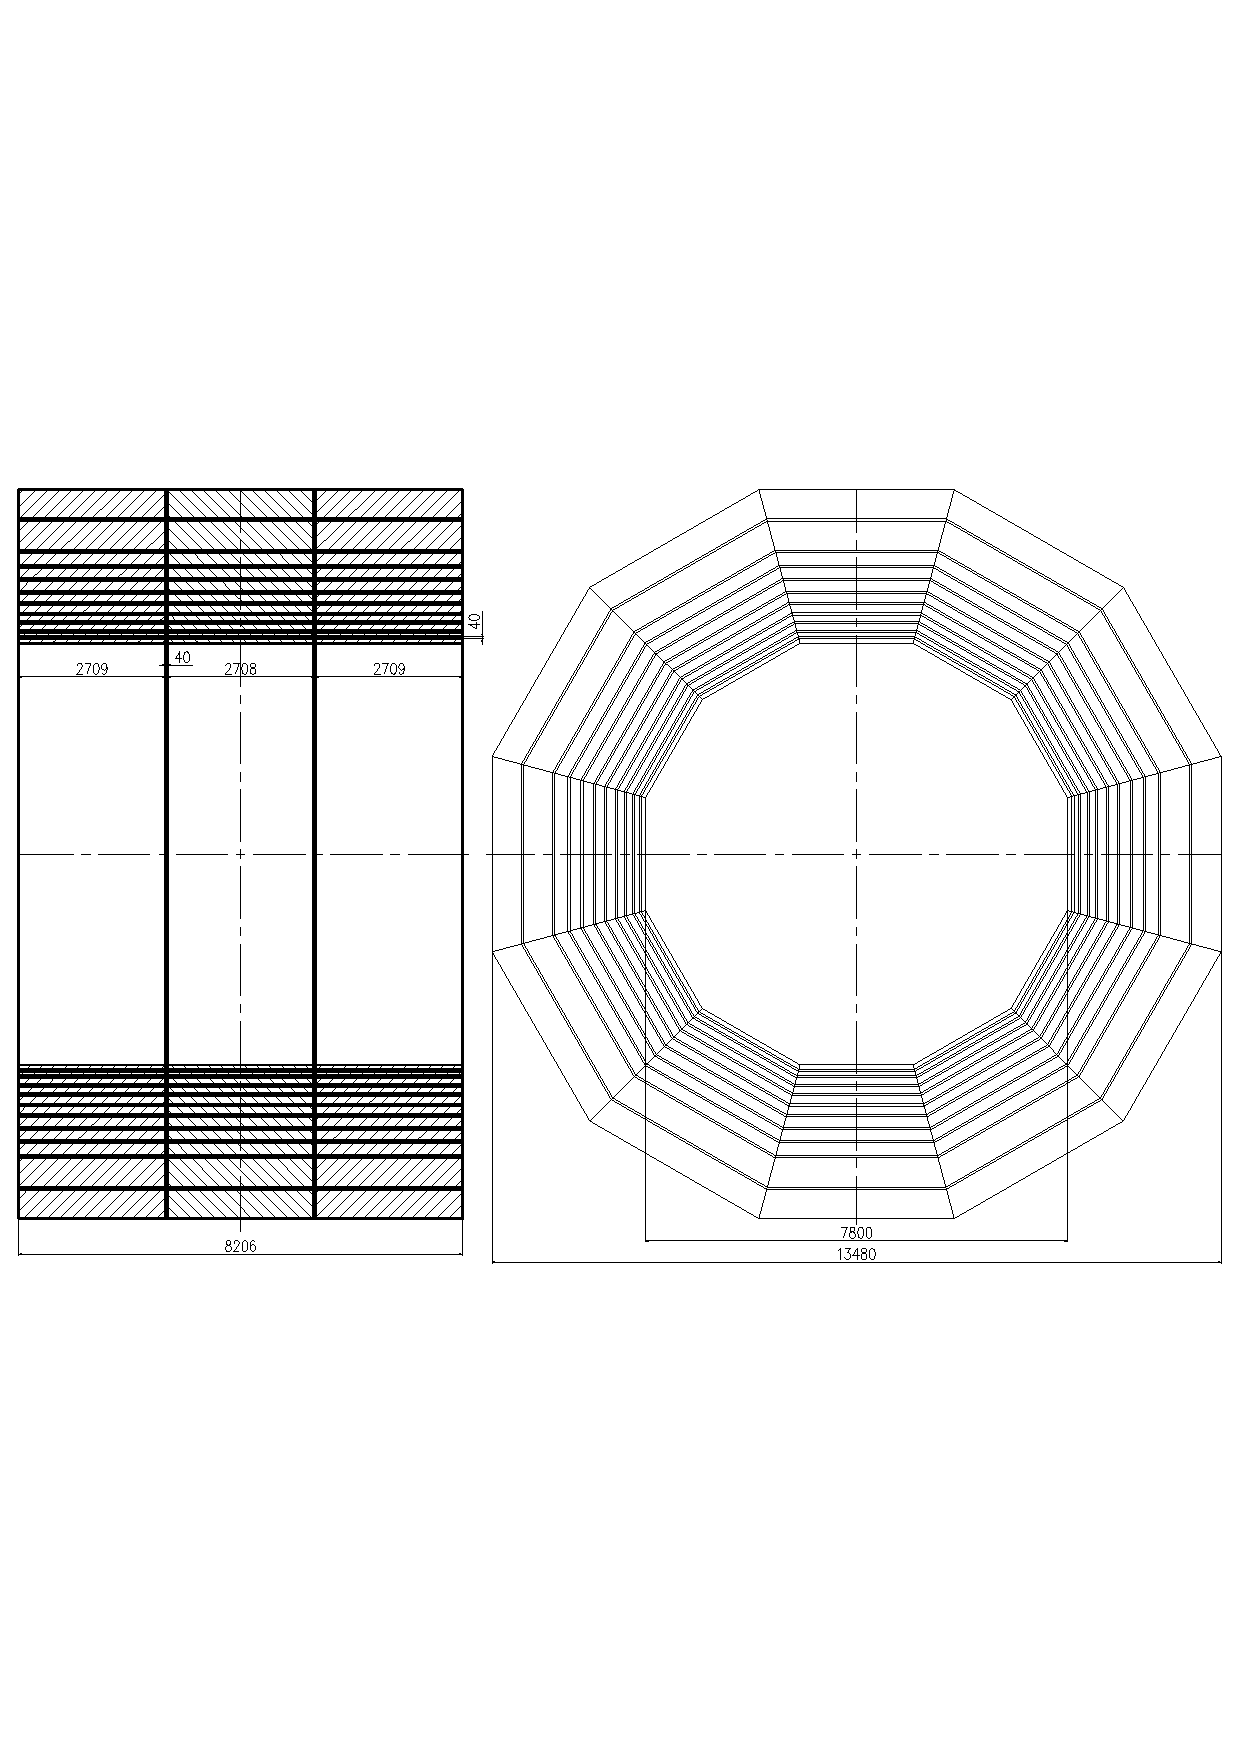
\includegraphics[scale=0.36]{Figures/Magnet/72}
\caption{iron design}
\label{fig:72}
\end{figure}

\subsection{The Endcap Yoke}


There are two endcap Yokes. Fig.3 shows the overall dimensions of them. The endcap yokes have a dodecagonal shape too. The inscribed circle diameter of the outer dodecagon will be 13300mm. The total thickness of the endcap will be 3150 mm. Each endcap yoke will consist of 7 layers. The thickness of the inner first layer is 600mm, and the second layer to the fourth layer is 100 mm and outer 3 layers are 200 mm. There will be 100 mm space between layers for muon detectors.


\begin{figure}[h!]
\centering
\includegraphics[scale=0.36]{Figures/Magnet/73}
\caption{iron design}
\label{fig:73}
\end{figure}


\subsection{Yoke assembly}
The total weight of the yoke will be about 10000 tons. Each ring of the barrel yoke and each endcap yoke will be composed of 12 segments. The maximum weight of the segments of the barrel yoke and endcap yoke will no more than 150 and 200 tons, respectively. The yoke will be preassembled at the manufacturer. Then they will be transported to the experimental site as segment. If there will be enough space, the yokes will be assembled at the IR hall. Otherwise they will be assembled in the surface building above the IR hall. The middle ring will be assembled together with the solenoid magnet. It will be the biggest one part to be lowered into the IR hall. Its weight will be about 3000 tons. A temporary gantry crane will be equipped. The time used for assembly at the IR hall will longer than that of assembly in the surface building.


\section{Dual Solenoid Scenario}


The active shielding design has been applied widely for commercial MRI magnets. Comparing to the one solenoid and yoke design, this design achieves a similar performance while being much lighter and more compact, which has been improved by FCC previous studies [1, 2]. Key to the choice of such magnets, in addition to their cost and complexity, is their ability to allow high-quality muon tracking. This is crucial for studying the properties of the Higgs boson, for example, and any additional new fundamental particles that await discovery. We will provide the active shielding conceptual design for Physicists to estimate its ability to allow high-quality particles tracking.


The active shielding design features two concentric antiseries connected superconducting solenoids, with the same room temperature bore as the one solenoid magnet mentioned in the chapter 6.2.1. The main solenoid provides 5 T central field over an obstruction-free room temperature bore of 7.2 m and a length of 7.6 m. The outer solenoid provides -2 T central field, with a radius of 6.5 m and a length of 10 m. The cold mass consists of two support cylinders for the main solenoid and shield solenoid (Fig. 6.8.1). The available areas for muon chambers are marked in the figure. The field map of the magnet is showed in Fig. 6.8.2, for consultation of particles tracking.

\begin{figure}[h!]
\centering
\includegraphics[scale=0.36]{Figures/Magnet/81}
\caption{Sketch figure for the half cross section of the active shielding magnet, with the available areas for muon chambers}
\label{fig:81}
\end{figure}

\begin{figure}[h!]
\centering
\includegraphics[scale=0.36]{Figures/Magnet/82}
\caption{Field map of the active shielding magnet}
\label{fig:82}
\end{figure}














\bibliographystyle{Style/atlasnote} %% plain.bst
\bibliography{Chapters/Magnet} %% bsample.bib

